% !TeX encoding = UTF-8
% !TeX spellcheck = en_US

\documentclass[fontset=mac]{thuthesis}
 
\input{thusetup}
\begin{document}
\begin{titlepage}
\newgeometry{top=1.55cm,bottom=2.2cm,left=2.55cm,right=2.55cm}
\thispagestyle{empty}

\vspace*{0.82cm}

\begin{center}
  
\includegraphics[width=10.8cm]{cover/log.jpg}

  \vspace{1.0cm}

  {\heiti\bfseries\fontsize{24pt}{30pt}\selectfont 课\ \ 程\ \ 大\ \ 作\ \ 业\ \ 说\ \ 明\ \ 书\par}
\end{center}

\vspace{0.75cm}

\begingroup
\setlength{\parindent}{0pt}
\fontsize{18pt}{28pt}\selectfont
\newcommand{\coverwideline}[1]{\underline{\makebox[13.7cm][c]{#1}}}
\newcommand{\coverinfoleft}[2]{\makebox[3.0cm][l]{#1}\underline{\makebox[3.65cm][c]{#2}}}
\newcommand{\coverinforight}[2]{\makebox[1.6cm][l]{#1}\underline{\makebox[3.3cm][c]{#2}}}

\begin{center}
  \coverwideline{大数据与云计算（Q）}\par
  \vspace{0.46cm}
  \coverwideline{CulCloud 云盘与大数据分析平台}\par
\end{center}

\vspace{1.48cm}

\begin{center}
\begin{minipage}{12.9cm}
  二级学院（直属学部）：\underline{\makebox[6.25cm][c]{计算机信息工程学院}}\par\vspace{0.42cm}
  \coverinfoleft{专业：}{软件工程}\hspace{0.3cm}\coverinforight{班级：}{23 软件一}\par\vspace{0.42cm}
  \coverinfoleft{学生姓名：}{曹磊}\hspace{0.3cm}\coverinforight{学号：}{23030301}\par\vspace{0.42cm}
  \coverinfoleft{学生姓名：}{陈佳明}\hspace{0.3cm}\coverinforight{学号：}{23030302}\par\vspace{0.42cm}
  \coverinfoleft{学生姓名：}{陈晓楠}\hspace{0.3cm}\coverinforight{学号：}{23030303}\par\vspace{0.42cm}
  \coverinfoleft{学生姓名：}{程志阳}\hspace{0.3cm}\coverinforight{学号：}{23030304}\par\vspace{0.42cm}
  \coverinfoleft{学生姓名：}{}\hspace{0.3cm}\coverinforight{学号：}{}\par
\end{minipage}
\end{center}
\endgroup

\vfill

\begin{center}
  {\songti\fontsize{16pt}{20pt}\selectfont 2026 年 6 月\par}
\end{center}
\restoregeometry
\end{titlepage}


\frontmatter
\begin{abstract}
  本文设计并实现了一个基于 Spark 与 Flask 的大数据分析与可视化系统。系统采用 Hadoop 生态存储海量数据，使用 Spark 进行高效的离线数据处理与分析，并通过 Flask 构建 RESTful API 服务，前端使用 React 框架实现数据的可视化展示。系统涵盖了数据采集、数据清洗、数据分析、数据可视化等完整的大数据处理流程，能够对用户行为数据、销售订单数据等多源数据进行多维度分析，并以图表形式直观呈现分析结果。实验结果表明，该系统能够有效处理 TB 级别的数据量，具有良好的可扩展性和实时响应能力。

  本系统的核心贡献包括：（1）设计了一套基于 Spark SQL 和 MLlib 的大数据分析流水线；（2）实现了基于 Flask 的 REST API 与前端可视化交互方案；（3）构建了完整的课程大作业报告模板，支持自动化编译。
\end{abstract}

\begin{abstract*}
  This paper designs and implements a big data analysis and visualization system based on Spark and Flask. The system adopts the Hadoop ecosystem for massive data storage, uses Spark for efficient offline data processing and analysis, builds RESTful API services through Flask, and implements data visualization on the frontend using the React framework. The system covers the complete big data processing workflow including data collection, data cleaning, data analysis, and data visualization. It can perform multi-dimensional analysis on multi-source data such as user behavior data and sales order data, and present the analysis results intuitively in the form of charts. Experimental results show that the system can effectively process TB-level data, with good scalability and real-time response capabilities.
\end{abstract*}


% 目录
\tableofcontents

% 插图和附表清单
% \listoffiguresandtables  % 插图和附表清单

% 正文部分
\mainmatter
\chapter{概述}

\section{项目背景}

随着信息技术的快速发展，各行各业产生的数据量呈指数级增长，大数据技术已成为推动社会进步和产业升级的关键力量。大数据分析与可视化作为大数据技术的重要应用方向，能够从海量数据中提取有价值的信息，并以直观的方式呈现给用户，辅助决策者做出更加科学的判断。

本课程大作业以"基于 Spark 与 Flask 的大数据分析与可视化系统"为题，旨在综合运用所学的大数据技术与 Web 开发技术，设计并实现一个完整的大数据处理与分析平台。

\section{项目目标}

本项目的主要目标包括：

\begin{enumerate}
  \item 掌握 Hadoop 分布式文件系统（HDFS）的部署与使用，实现海量数据的分布式存储；
  \item 掌握 Spark 计算框架的基本原理与编程模型，实现大规模数据的高效处理与分析；
  \item 掌握 Flask Web 框架的使用，构建 RESTful API 服务；
  \item 掌握数据可视化技术，使用 ECharts 等工具实现分析结果的可视化展示；
  \item 综合运用以上技术，构建一个完整的大数据分析与可视化系统。
\end{enumerate}

\section{项目范围}

本项目涵盖数据采集、数据存储、数据处理、数据分析、数据可视化等完整的大数据链路，具体包括：

\begin{itemize}
  \item 数据层：模拟生成用户行为数据和销售订单数据，存储在 HDFS 中；
  \item 计算层：使用 Spark SQL 进行数据清洗与转换，使用 Spark MLlib 进行数据分析与挖掘；
  \item 服务层：使用 Flask 构建 RESTful API，提供数据查询与统计分析接口；
  \item 展示层：使用 React + ECharts 构建可视化仪表盘，实时展示分析结果。
\end{itemize}

\chapter{相关软件及技术简介}

本章介绍 CulCloud 平台开发过程中使用的主要技术，包括前端框架、后端服务、对象存储、任务队列、文件转换、PDF 渲染和大数据分析组件。

\section{前端开发技术}

\subsection{React 组件化开发}

\begin{figure}[H]
  \centering
  
\includegraphics[width=0.42\textwidth,height=3.2cm,keepaspectratio]{logos-pdf/logo-react.pdf}
  \caption{React 标识}
  \label{fig:chap02-react-logo}
\end{figure}

前端采用 React 框架构建模块化的单页面应用\cite{reactdocs}。系统将 Dashboard、MyFiles、ConvertCenter、PDFStudio 等业务视图抽象为独立组件，并设计了全局 DashboardContext 机制（见 file-cloud-frontend/src/context/useDashboard.tsx），统一维护视图流转与用户角色。在角色切换时，系统触发组件树重渲染，并在顶层容器动态绑定 theme-admin 样式，实现界面主题与视图权限的平滑过渡。

\subsection{TypeScript 类型约束}

\begin{figure}[H]
  \centering
  
\includegraphics[width=0.38\textwidth,height=3cm,keepaspectratio]{logos-pdf/logo-typescript.pdf}
  \caption{TypeScript 标识}
  \label{fig:chap02-typescript-logo}
\end{figure}

系统引入 TypeScript 进行静态类型约束，所有通信接口与状态协议均在 file-cloud-frontend/src/types.ts 中定义。通过对 FileItem、Task 等核心数据结构进行显式建模，在编译期捕获类型不匹配与属性缺失问题，保障文件预览、异步转换等多分支业务流转时的运行时稳定性。

\subsection{Vite 与界面构建}

\begin{figure}[H]
  \centering
  
\includegraphics[width=0.38\textwidth,height=3cm,keepaspectratio]{logos-pdf/logo-vite.pdf}
  \caption{Vite 标识}
  \label{fig:chap02-vite-logo}
\end{figure}

Vite 负责前端代码的开发调试与最终构建。利用其原生的 ESM 按需编译能力提升频繁交互界面（如 PDF 批注工作区）的响应开发效率。构建产物输出为优化后的静态资源，交由服务端托管部署。

\subsection{HTML5 Canvas 交互渲染}

\begin{figure}[H]
  \centering
  
\includegraphics[width=0.34\textwidth,height=2.7cm,keepaspectratio]{logos-pdf/logo-html5-canvas.pdf}
  \caption{HTML5 Canvas 标识}
  \label{fig:chap02-canvas-logo}
\end{figure}

HTML5 Canvas 是 PDF 工作区与管理驾驶舱的可视化基础\cite{mdncanvas}。在 PDF 批注中，系统在 Canvas 层上记录用户画笔、矩形和文本的相对坐标，并在导出时传给后端换算。同时，管理端 ECharts 默认采用 CanvasRenderer 绘制拓扑与统计图表，提供高效的可视化呈现。

\section{后端服务技术}

\subsection{FastAPI 接口服务}

\begin{figure}[H]
  \centering
  
\includegraphics[width=0.38\textwidth,height=3cm,keepaspectratio]{logos-pdf/logo-fastapi.pdf}
  \caption{FastAPI 标识}
  \label{fig:chap02-fastapi-logo}
\end{figure}

后端基于 FastAPI 构建高效的 REST API 路由\cite{fastapi}。利用 Pydantic 结构化校验前端提交的各类请求（如 PDF 页面重组请求，详见 backend/app/models/schemas.py），确保路由入口层的数据安全性；配合依赖注入机制，解耦鉴权、MinIO 客户端与任务状态调度逻辑。

\subsection{Flask 分析服务}

\begin{figure}[H]
  \centering
  
\includegraphics[width=0.34\textwidth,height=2.7cm,keepaspectratio]{logos-pdf/logo-flask.pdf}
  \caption{Flask 标识}
  \label{fig:chap02-flask-logo}
\end{figure}

Flask 框架用于承载独立的分析数据接口\cite{flaskdocs}。该分析服务与 FastAPI 解耦，专门用于读取 Spark 分布式聚合产物及服务遥测数据，并将其映射为管理驾驶舱所消费的历史指标接口，从而实现主业务流与分析遥测流在架构上的分层。

\subsection{Redis 与 Celery 任务队列}

\begin{figure}[H]
  \centering
  \begin{minipage}{0.38\textwidth}
    \centering
    
\includegraphics[height=3cm,keepaspectratio]{logos-pdf/logo-redis.pdf}
  \end{minipage}
  \hspace{0.08\textwidth}
  \begin{minipage}{0.38\textwidth}
    \centering
    
\includegraphics[height=3cm,keepaspectratio]{logos-pdf/logo-celery.pdf}
  \end{minipage}
  \caption{Redis 与 Celery 标识}
  \label{fig:chap02-redis-celery-logo}
\end{figure}

Redis 与 Celery 协同实现文件转换的异步任务队列。Redis 作为消息 Broker 并缓存近期任务的运行状态（含 queued, processing, success, failed，详见 backend/app/services/task\_queue.py）。通过将计算密集型的文档转换（如 LibreOffice 转换）从同步 HTTP 请求中解耦，前端可发起状态轮询展示进度，保证了核心接口的响应性能。

\subsection{MinIO 对象存储}

\begin{figure}[H]
  \centering
  
\includegraphics[width=0.42\textwidth,height=3.2cm,keepaspectratio]{logos-pdf/logo-minio.pdf}
  \caption{MinIO 标识}
  \label{fig:chap02-minio-logo}
\end{figure}

系统采用 MinIO 充当本地对象湖存储\cite{minio}。后端通过“对象名路径前缀”（详见 backend/app/routers/folders.py）模拟分层文件夹，重命名或移动时，级联拷贝前缀匹配的所有对象再批量清除源对象，在对象存储扁平架构上提供了高效的层级文件目录视图。

\section{文件处理技术}

\subsection{Office 与 PDF 转换}

\begin{figure}[H]
  \centering
  \begin{minipage}{0.38\textwidth}
    \centering
    
\includegraphics[height=3cm,keepaspectratio]{logos-pdf/logo-libreoffice.pdf}
  \end{minipage}
  \hspace{0.08\textwidth}
  \begin{minipage}{0.38\textwidth}
    \centering
    
\includegraphics[height=3cm,keepaspectratio]{logos-pdf/logo-gotenberg.pdf}
  \end{minipage}
  \caption{LibreOffice 与 Gotenberg 标识}
  \label{fig:chap02-libreoffice-gotenberg-logo}
\end{figure}

系统集成 Gotenberg 转换服务处理异构文档格式\cite{gotenberg}。该服务容器化集成了 LibreOffice 和 PDF 引擎，后端通过 HTTP 接口提交 Office 转 PDF 任务，避免了直接在主业务进程中拉起本地进程的开销，结合 P0 格式白名单确保转换队列的可靠运行。

\subsection{CSV、Markdown 与文本渲染}

对于 CSV、Markdown 和 TXT 等轻量文本，系统采用本地轻量解析技术。后端直接提取文本并将其渲染为隔离的 HTML，前端通过预览容器直接呈现，无需触发繁重的文档转换流程。

\subsection{PDF 页面渲染与批注}

\begin{figure}[H]
  \centering
  
\includegraphics[width=0.38\textwidth,height=3cm,keepaspectratio]{logos-pdf/logo-pdfjs.pdf}
  \caption{PDF.js 标识}
  \label{fig:chap02-pdfjs-logo}
\end{figure}

对于 PDF 页面渲染与管理，系统以 PDF.js 的逻辑视口机制作为设计参照\cite{pdfjs}。PDFStudio 采用双层画布模型：底层展示后端 PyMuPDF 导出的高清页面图像，上层在 HTML5 Canvas 叠加手写及文本批注。前端记录相对视口的逻辑坐标与分辨率，导出时由后端进行坐标变换并合并写入新文件。

\section{运行与部署技术}

\subsection{PM2 进程管理}

\begin{figure}[H]
  \centering
  
\includegraphics[width=0.40\textwidth,height=3cm,keepaspectratio]{logos-pdf/logo-pm2.pdf}
  \caption{PM2 标识}
  \label{fig:chap02-pm2-logo}
\end{figure}

PM2 用于管理应用层的前端与分析模块服务\cite{pm2docs}。根目录下的 ecosystem.config.js 统一配置了开发与生产的服务进程。PM2 支持异常退出自动拉起与集中日志查阅，保障本地开发和现场验证时的服务连续性。

\subsection{Docker Compose 容器编排}

\begin{figure}[H]
  \centering
  
\includegraphics[width=0.40\textwidth,height=3cm,keepaspectratio]{logos-pdf/logo-docker-compose.pdf}
  \caption{Docker Compose 标识}
  \label{fig:chap02-docker-compose-logo}
\end{figure}

Docker Compose 用于编排系统底层的 Redis、MinIO、Gotenberg 及 API 镜像\cite{dockerdocscompose}。通过将持久化存储挂载、网络端口与多服务拓扑写入 docker-compose.yml 声明式配置，系统形成了“PM2 监管上层应用、Compose 监管基础设施”的混合部署架构。

\section{大数据分析技术}

\subsection{HDFS 与 Spark}

\begin{figure}[H]
  \centering
  \begin{minipage}{0.38\textwidth}
    \centering
    
\includegraphics[height=3cm,keepaspectratio]{logos-pdf/logo-apache-hadoop.pdf}
  \end{minipage}
  \hspace{0.08\textwidth}
  \begin{minipage}{0.38\textwidth}
    \centering
    
\includegraphics[height=3cm,keepaspectratio]{logos-pdf/logo-apache-spark.pdf}
  \end{minipage}
  \caption{Hadoop 与 Spark 标识}
  \label{fig:chap02-hadoop-spark-logo}
\end{figure}

HDFS 与 Spark 构成了本平台的大数据离线遥测分析管线\cite{shvachko2010hdfs,zaharia2016spark}。遥测流水日志进入存储后，Spark 计算引擎执行周期性的数据清洗、操作统计、错误率计算和格式流转矩阵分析，聚合出的指标存入静态 JSON，打通了“业务日志-数据清洗-指标分析-结果应用”的数据流。

\subsection{ECharts 可视化}

\begin{figure}[H]
  \centering
  
\includegraphics[width=0.38\textwidth,height=3cm,keepaspectratio]{logos-pdf/logo-apache-echarts.pdf}
  \caption{Apache ECharts 标识}
  \label{fig:chap02-echarts-logo}
\end{figure}

前端集成 ECharts 图表库进行多维度数据呈现。通过对实时事件流与 Spark 历史数据进行提取，使用折线图展示流量趋势、柱状图展示格式分布、雷达图展示质量监控、Sankey 拓扑图展示格式流转，提升了管理端驾驶舱的可视化运营密度。

\section{团队分工与协作机制}

为确保 CulCloud 云盘与大数据分析平台各项复杂技术的顺利落地与系统级集成，项目团队制定了高度工程化的团队分工与协作机制。各小组成员具体分工如下：

\textbf{曹磊（组长）}：全面负责系统的基础架构设计与核心后端开发。设计并实现了基于 FastAPI 的 REST API 接口体系、MinIO 级联目录与对象湖迁移逻辑、Redis 与 Celery 异步任务队列调度，以及 Gotenberg 文档转换引擎的容器化集成；同时，主导了基于 Apache Spark 的分布式离线分析管线，设计了管理驾驶舱的实时拓扑图与运行日志流面板，并编写了覆盖系统核心交互链路的 11 项 E2E 自动化测试用例，为代码集成合并提供了严格的质量保障。

\textbf{陈佳明（组员）}：负责用户端基础页面与文件管理前端交互开发。实现了“个人首页”与“我的文件”模块的前端渲染，包括多维度分类过滤器、路径面包屑导航、文件拖拽上传列表等 React 组件编写，并完成了全站的 CSS 样式适配与响应式布局调整，实现了用户端界面的平滑流转。

\textbf{陈晓楠（组员）}：负责 PDF Studio 处理面板前端视图开发。实现了 PDF 卡片拖拽重排与旋转/删除的状态管理，编写了 Canvas 轻量化手写及文本批注交互逻辑，并与组长协作调试了前端视口逻辑坐标到后端物理 PDF 页面坐标的换算与批注写回逻辑。

\textbf{程志阳（组员）}：负责格式转换控制台与分析接口辅助开发。实现了“转换中心”前端面板，编写了格式转换任务提交与基于定时器的状态轮询终止逻辑，同时协助组长开发了 Flask 离线分析微服务中的指标读取与遥测数据查询接口。

为了在系统验收与评审中展现系统工程的严密性，防止因代码细节引发追问，团队制定了高度工程化的协作与版本管理策略。首先，团队采用 Schema-First（接口先行）协作模式，开发初期通过 FastAPI 的 OpenAPI 文档，基于 Pydantic 明确定义了所有 API 请求与响应的 JSON 数据格式（Schema），形成了前后端的强契约关系，允许前端组员使用 Mock 数据并行开发视图，而组长在后端同步实现真实业务逻辑。其次，在版本管理上采用 Git Flow 分支管理规范，由组长曹磊维护主分支 v2-platform，组员分别在各自的特性分支（如 feat-myfiles、feat-pdfstudio）上独立进行提交，互不干扰。最终在分支合并时，组员必须在本地运行通过组长编写的 Playwright 自动化测试集，所有用例通过后方可由组长合并至主分支，通过严密的质量网关保障了代码的稳定集成。

\section{本章小结}

本章介绍了系统涉及的前端、后端、对象存储、任务队列、文件转换、PDF 渲染、运行部署和大数据分析技术。这些技术共同支撑 CulCloud 从单纯文件列表扩展为可上传、可预览、可转换、可编辑和可分析的资料处理平台。

从工程分层看，React、TypeScript、Vite 和 Canvas 负责构建浏览器侧的高交互界面，FastAPI 负责承载文件处理主链路，Flask 则作为轻量分析服务承担驾驶舱数据接口，二者形成“主业务服务”和“分析辅助服务”的边界。Redis 与 Celery 将耗时转换任务从同步请求中拆离，MinIO 负责对象化存储，Gotenberg、LibreOffice 和 PDF.js 分别补足 Office 转换、PDF 生成和页面渲染能力。PM2 与 Docker Compose 的组合则对应本地展示和容器化依赖两类运行场景，使系统既能快速预览，也能保持转换、缓存和对象存储等基础服务的可复现性。

这些技术并不是孤立堆叠，而是围绕文件流转闭环进行组合：用户上传资料后，后端写入对象存储并记录元数据；需要预览或转换时，任务队列调度转换服务生成结果；需要批注时，前端通过 PDF 页面图和 Canvas 批注层维护坐标关系；需要管理分析时，日志与遥测数据进入 Spark 聚合链路并由 ECharts 呈现。后续章节将在此基础上进一步说明需求建模、总体架构、核心模块实现和测试验证方法。

\chapter{系统分析与总体设计}

\section{需求分析}

系统用户分为学生用户、教师/评委和管理员三类。学生用户关注上传、分类、预览、转换和 PDF 编辑；教师/评委关注系统是否具备真实功能和可演示证据；管理员关注任务队列、失败任务、系统健康和数据驾驶舱。

\section{功能模块设计}

\begin{table}[htbp]
  \centering
  \caption{系统功能模块划分}
  \label{tab:function-modules}
  \begin{tabular}{lll}
    \toprule
    模块 & 主要功能 & 数据来源 \\
    \midrule
    个人首页 & 文件数、空间、转换成功、失败任务 & 文件 API、任务 API \\
    我的云盘 & 上传、分类、预览、下载、重命名、删除 & MinIO/HDFS \\
    转换中心 & Office/PDF/图片/Markdown 转换 & 转换 API、任务队列 \\
    PDF 编辑室 & 预览、批注、页面整理、打印导出 & PDF 页面提取 API \\
    管理驾驶舱 & 遥测分析、质量指标、拓扑与状态 & Spark 聚合数据 \\
    系统状态 & 服务健康、队列长度、近期失败 & health/task/log API \\
    \bottomrule
  \end{tabular}
\end{table}

\section{数据流设计}

用户上传文件后，前端调用文件上传 API，将文件写入对象存储。预览模块根据文件类型生成 PDF、图片、文本或 HTML 预览内容。转换中心提交异步任务，任务完成后生成转换产物并写回云盘。PDF 编辑室加载 PDF 页面图，前端记录批注对象；页面重排导出由后端根据页面配置生成新 PDF，批注打印导出由浏览器打印渲染完成。

\section{合规与安全设计}

系统采用以下安全设计：上传和预览接口分离，避免预览缓存覆盖原文件；文件删除和重命名由用户主动触发；Dashboard 在接口失败时展示不可用状态而不是假数据；通知面板只展示真实失败任务；日志仅用于实验追踪和异常定位。

\section{数据库与对象结构}

系统文件实体包含 \texttt{object\_name}、\texttt{filename}、\texttt{size}、\texttt{last\_modified} 和 \texttt{content\_type}。任务实体包含 \texttt{task\_id}、\texttt{kind}、\texttt{status}、\texttt{created\_at}、\texttt{completed\_at}、\texttt{error} 和 \texttt{result\_url}。这些字段支撑首页真实指标、任务列表、失败通知和文档测试表。


\chapter{系统总体设计}

本章从总体架构、功能模块、业务流程、数据结构和部署结构五个方面说明 CulCloud 的系统设计。设计目标不是简单堆叠页面功能，而是让用户端文件处理、后端任务状态、对象存储、运行日志和管理端分析形成一致的数据闭环。系统采用 React 前端、FastAPI 业务服务、MinIO 对象存储、Redis 状态与日志、Gotenberg 转换服务以及 Flask/Spark 分析服务的组合结构，使文件上传、预览、转换、PDF 页面整理和管理端观察能够在同一平台内协同运行。

\section{总体架构设计}

CulCloud 按照表示层、业务接口层、领域服务层、基础数据层和分析应用层进行分层。表示层包含用户端与管理端两类界面，用户端负责文件上传、目录整理、预览、格式转换和 PDF 编辑，管理端负责任务、日志、健康状态和分析结果观察。业务接口层由 FastAPI 提供统一入口，按文件、目录、预览、转换、任务、日志和系统健康拆分路由。领域服务层封装对象存储、文档转换、任务追踪、日志采集和健康检查。基础数据层由 MinIO、Redis 和 Gotenberg 构成，分别承担对象保存、状态保存和文档渲染转换。历史分析层由 Spark 输出聚合 JSON，Flask Analytics 提供读取接口，再由管理端 ECharts 呈现。

图 \ref{fig:chap04-layer-architecture} 给出了系统分层架构。该图强调两类数据口径：第一类是 FastAPI 直接聚合的实时运行数据，来自文件、任务、日志和系统健康接口；第二类是 Spark 处理后的历史分析样本，用于展示较长时间窗口下的文件类型、转换趋势和质量指标。二者在管理端同时出现，但语义上保持分离，避免将离线样本误认为实时业务总量。

\begin{figure}[H]
  \centering
  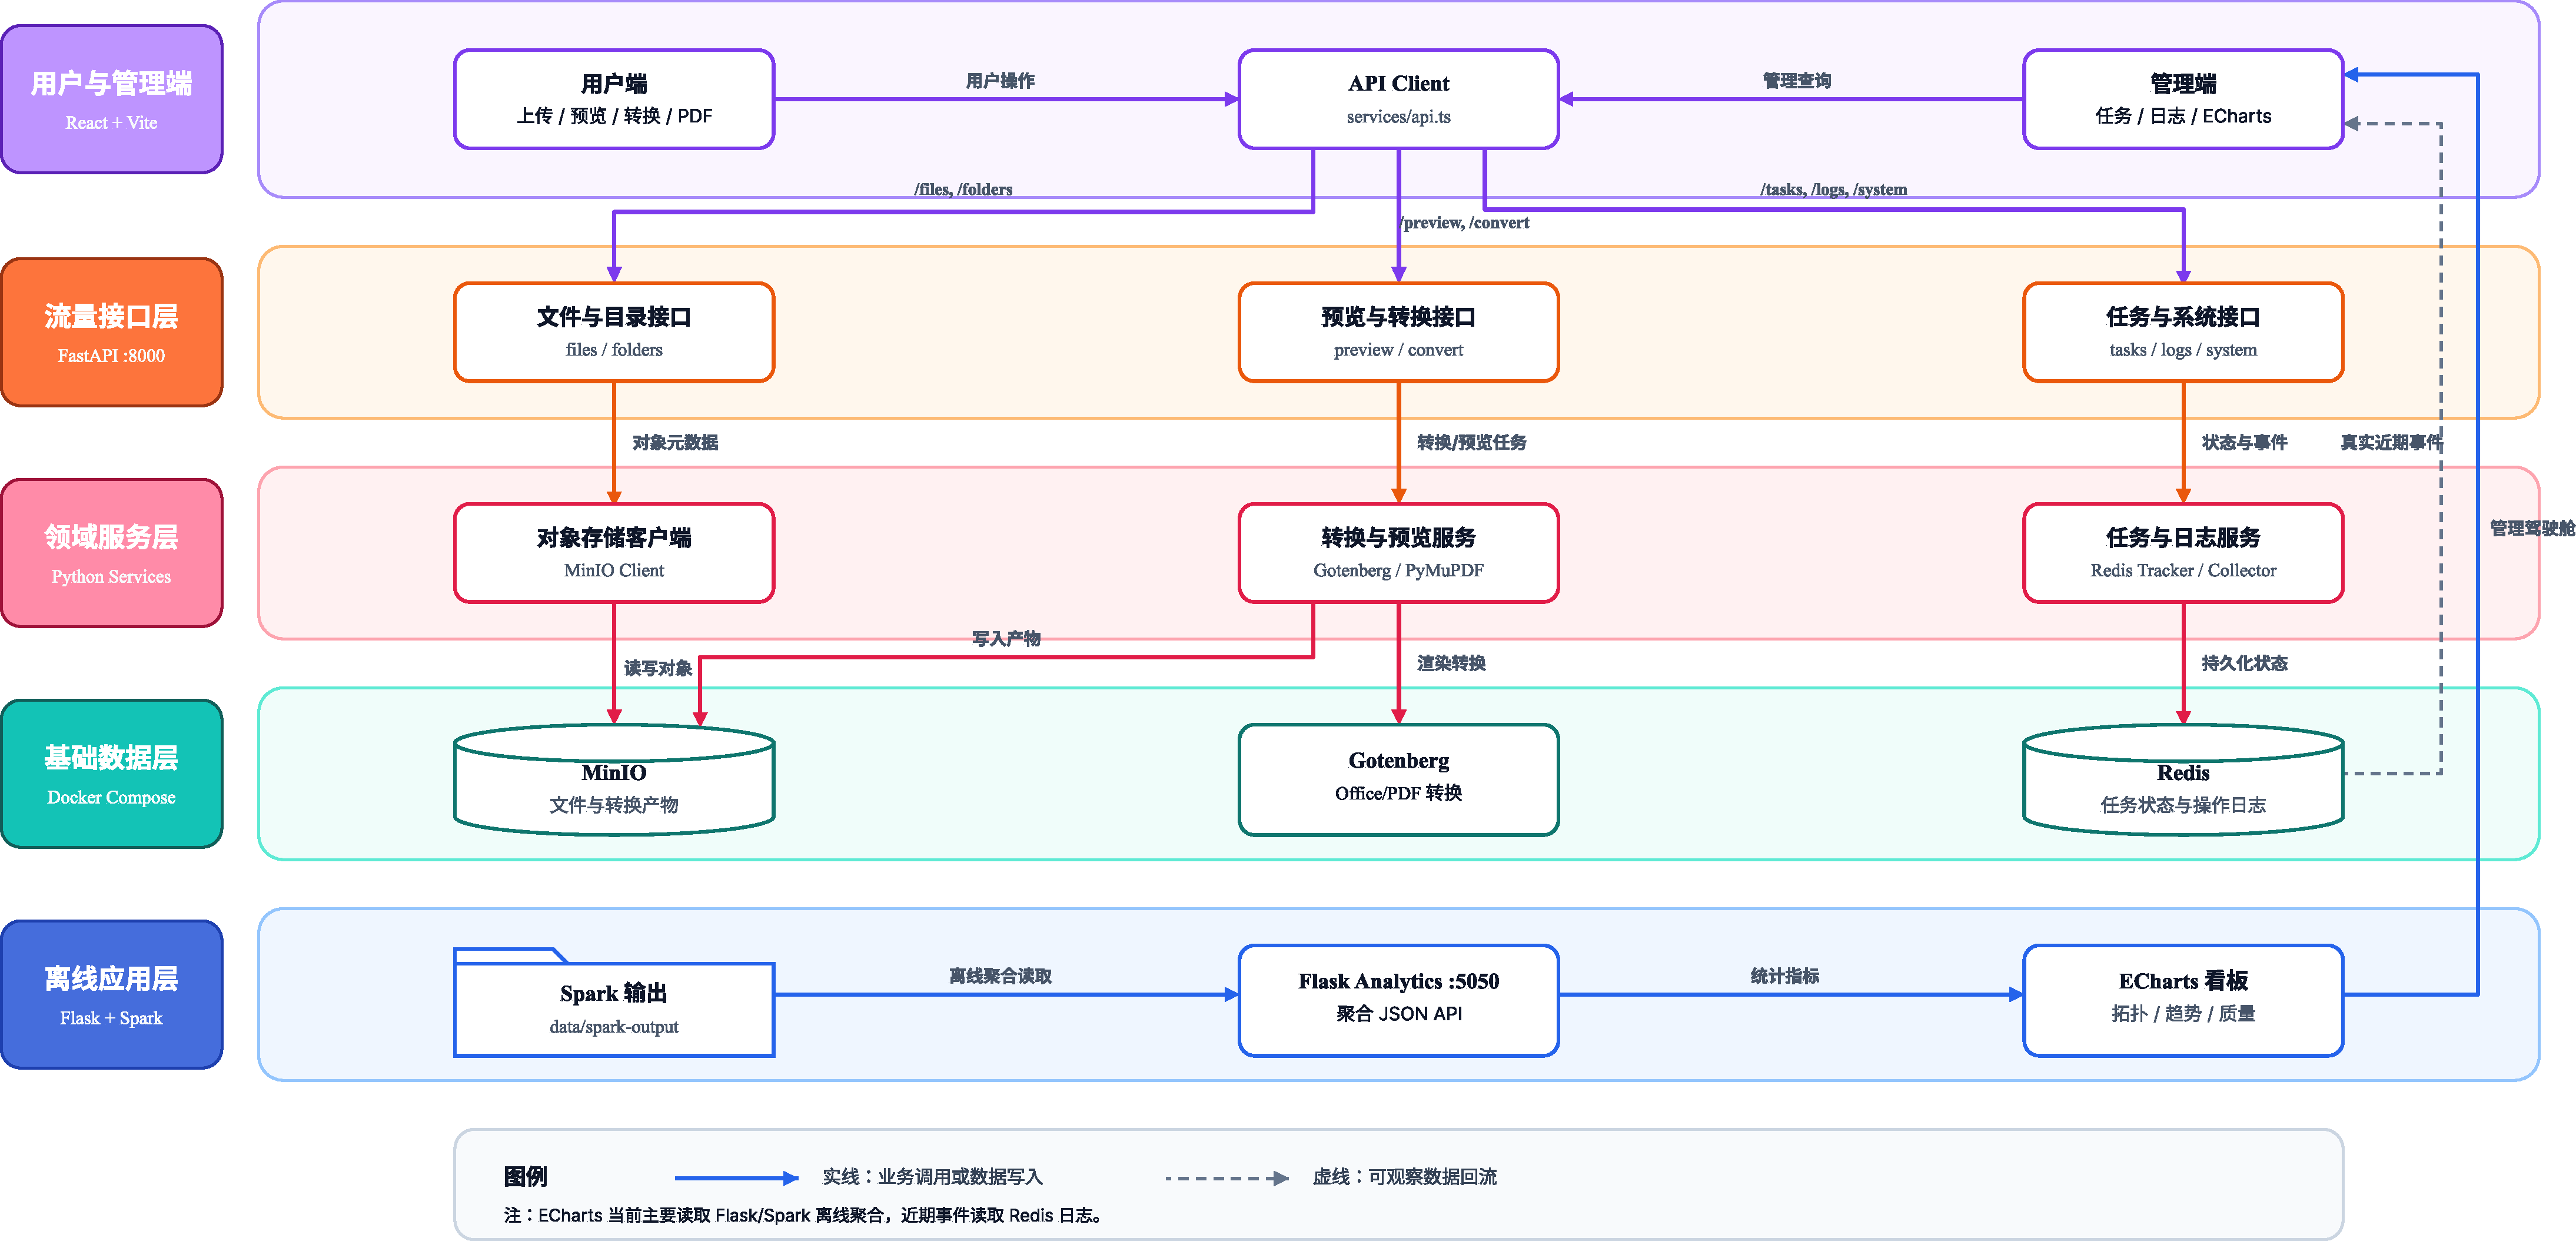
\includegraphics[width=0.96\textwidth,height=0.62\textheight,keepaspectratio]{figures-pdf/fig08-云端资料处理平台系统分层架构图.pdf}
  \caption{云端资料处理平台系统分层架构图}
  \label{fig:chap04-layer-architecture}
\end{figure}

\section{系统功能设计}

\subsection{功能模块划分}

系统围绕用户端和管理端两条主线划分为六个核心模块。用户端包含个人首页、我的文件、转换中心和 PDF 编辑室；管理端包含管理驾驶舱、任务监控和系统状态。各模块并非孤立页面，而是通过统一 API 客户端访问后端接口，再由后端服务读写 MinIO 与 Redis。表 \ref{tab:function-modules} 列出了模块边界与数据来源。

\begin{table}[H]
  \centering
  \caption{系统功能模块划分}
  \label{tab:function-modules}
  \begin{tabularx}{\textwidth}{llXX}
    \toprule
    端侧 & 模块 & 主要功能 & 数据来源 \\
    \midrule
    用户端 & 个人首页 & 文件数量、空间占用、近期任务和失败提示 & 文件接口、任务接口 \\
    用户端 & 我的文件 & 上传、目录、搜索、移动、删除和下载 & MinIO 对象元数据 \\
    用户端 & 文件预览 & PDF、图片、文本、Markdown、CSV、Office、音视频预览 & 预览接口、转换缓存 \\
    用户端 & 转换中心 & P0 白名单格式转换、任务轮询、结果下载 & 转换接口、Redis 任务状态 \\
    用户端 & PDF 编辑室 & 页面提取、排序、旋转、删除、批注和导出 & PDF 处理接口、MinIO 产物 \\
    管理端 & 管理驾驶舱 & 实时运行状态、历史分析样本和图表展示 & FastAPI、Flask/Spark、ECharts \\
    \bottomrule
  \end{tabularx}
\end{table}

图 \ref{fig:chap04-module-dependency} 展示了模块依赖关系。前端不直接访问 MinIO、Redis 或 Gotenberg，而是通过 API 客户端进入 FastAPI 路由，由路由层调用领域服务完成对象读写、转换执行和状态记录。这种设计将浏览器侧交互与基础设施细节隔离，降低了前端暴露存储地址或内部任务键的风险。

\begin{figure}[H]
  \centering
  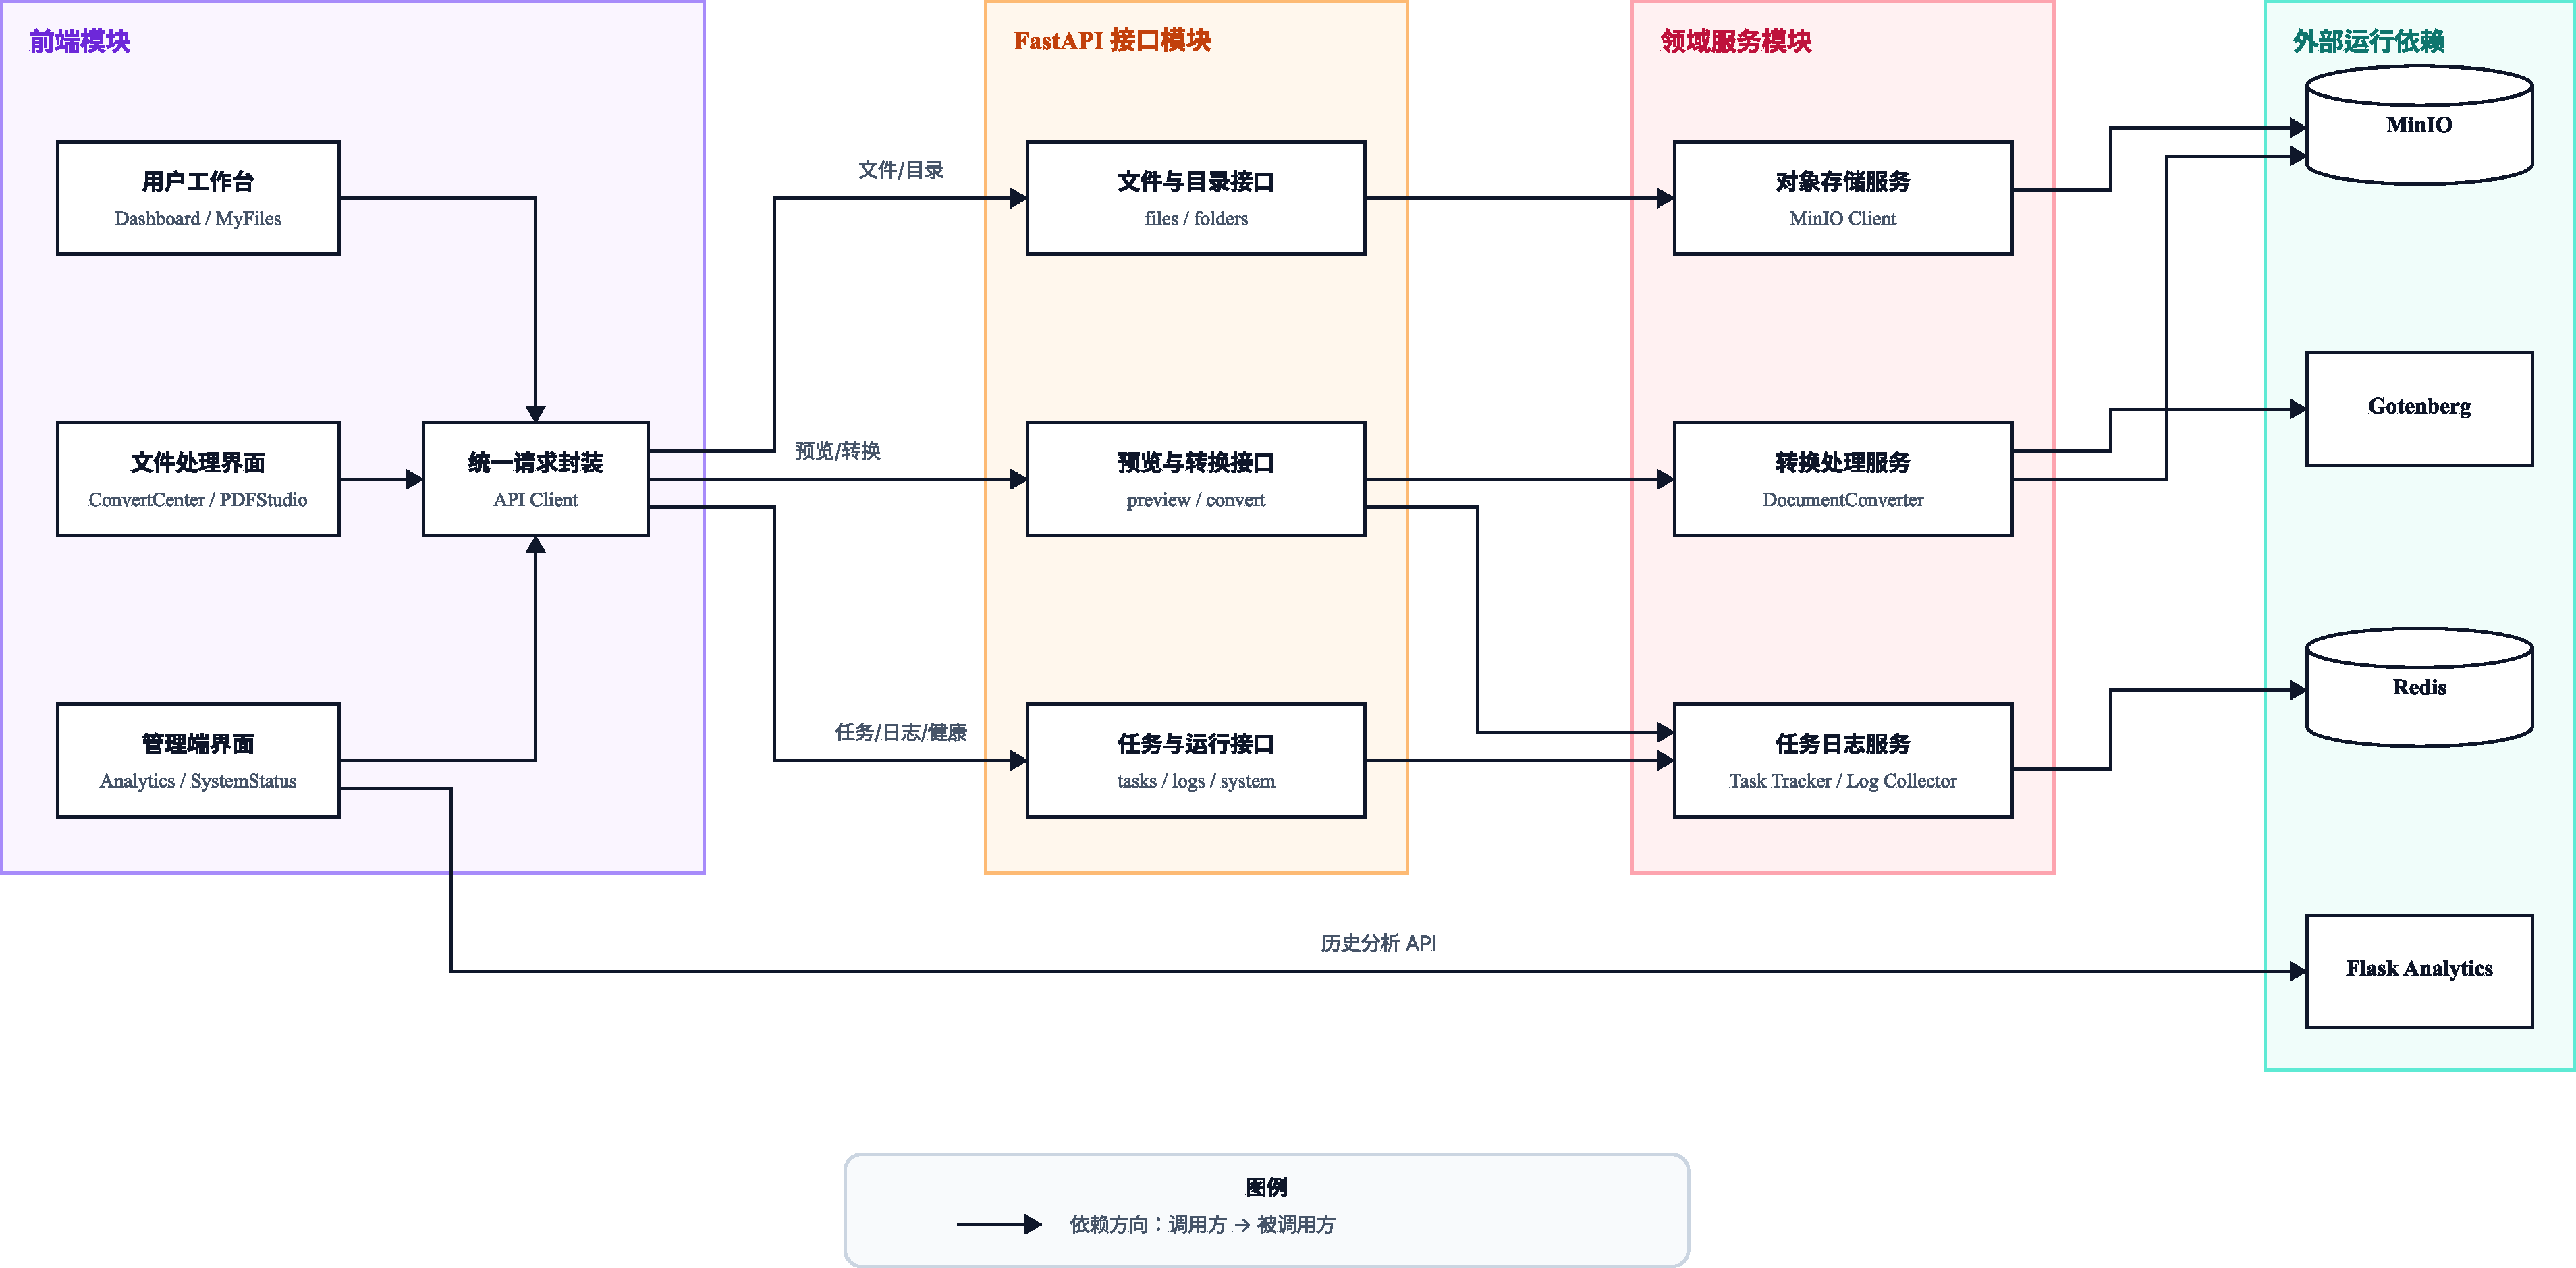
\includegraphics[width=0.96\textwidth,height=0.52\textheight,keepaspectratio]{figures-pdf/fig09-moudules-diagrams.pdf}
  \caption{前后端核心模块依赖图}
  \label{fig:chap04-module-dependency}
\end{figure}

\subsection{用户端模块}

用户端的设计重点是让普通用户以云盘方式组织资料，并在同一界面路径中完成处理。我的文件模块负责对象列表、目录前缀、类型筛选和预览入口；转换中心负责从本地或云端选择文件，按白名单提交格式转换任务；PDF 编辑室负责将 PDF 页面转为可操作页面集合，再提交页面顺序、旋转角度和批注配置生成新文件。用户端所有可生成产物的操作都应写入任务状态和事件日志，以便后续查询与管理端观察。

\subsection{管理端模块}

管理端的设计重点是观察系统运行，而不是重复用户端操作。第一屏读取 FastAPI 的文件、任务、日志和健康接口，显示当前业务系统真实状态；第二屏和第三屏读取 Spark 历史分析样本，展示文件类型分布、历史转换任务、遥测质量、存储水位和错误热力图。任务监控用于查看任务列表、队列长度和失败原因；系统状态用于观察 Redis、MinIO、Gotenberg、API 和分析服务的健康状态。

\section{业务流程设计}

系统核心业务并不是单个页面动作，而是“用户操作、后端处理、对象产物、任务状态、管理观察”的闭环。用户端上传、预览、转换和 PDF 导出会进入 FastAPI 路由，后端根据任务类型读写 MinIO 对象，并将任务状态与事件日志写入 Redis；管理端第一屏再从文件、任务、日志和健康接口读取实时数据。图 \ref{fig:chap04-business-loop} 展示了这一业务闭环，它用于说明用户端业务增量为什么能够实时反映到管理端运行指标中。

\begin{figure}[H]
  \centering
  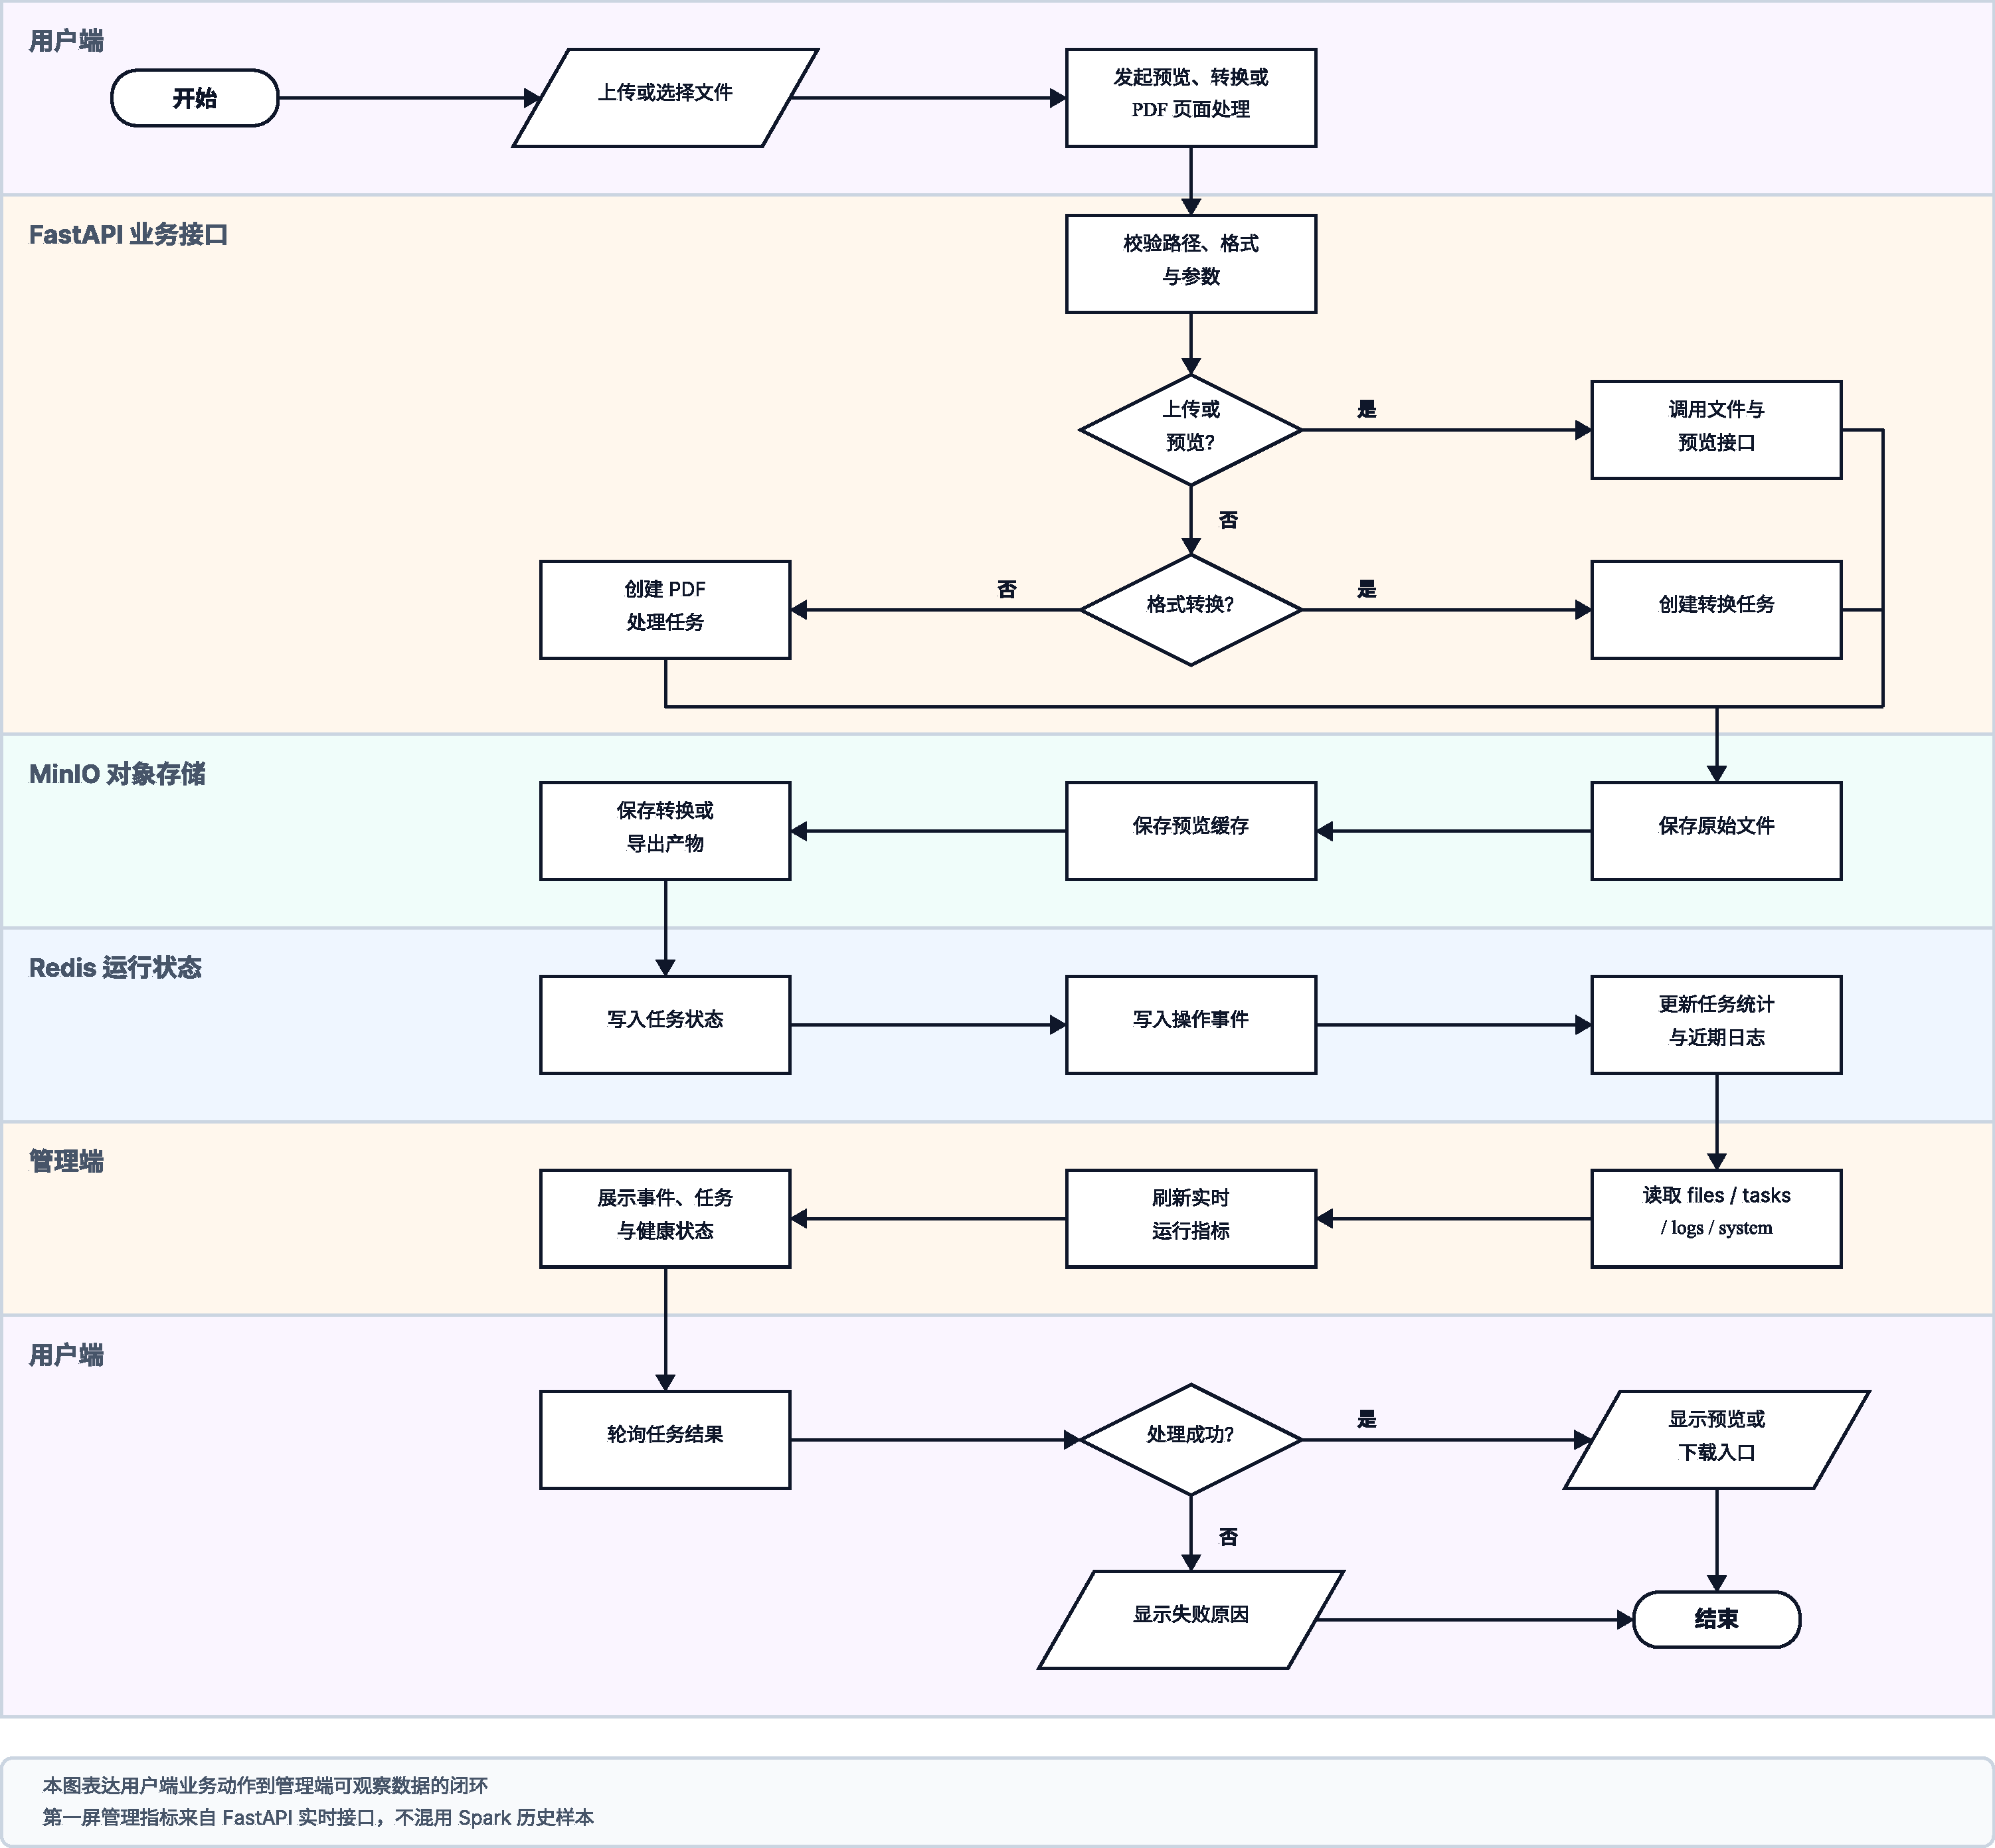
\includegraphics[width=0.96\textwidth,height=0.58\textheight,keepaspectratio]{figures-pdf/fig16-核心业务闭环流程图.pdf}
  \caption{核心业务闭环流程图}
  \label{fig:chap04-business-loop}
\end{figure}

\subsection{文件上传与预览流程}

文件上传流程从用户选择文件开始。前端携带当前目录前缀和相对路径调用上传接口，后端校验路径合法性后生成对象名称，将文件写入 MinIO，并记录上传事件。列表刷新时，后端根据对象名前缀和 \texttt{.keep} 空对象合成文件夹与文件视图。预览流程则由文件类型决定：图片、PDF、音频和视频可直接返回内容地址；TXT、Markdown 和 CSV 由后端生成可读内容；Office 文件优先生成 PDF 预览缓存。图 \ref{fig:chap04-preview-flow} 用活动图表示了上传、列表刷新和预览之间的责任边界。

\begin{figure}[H]
  \centering
  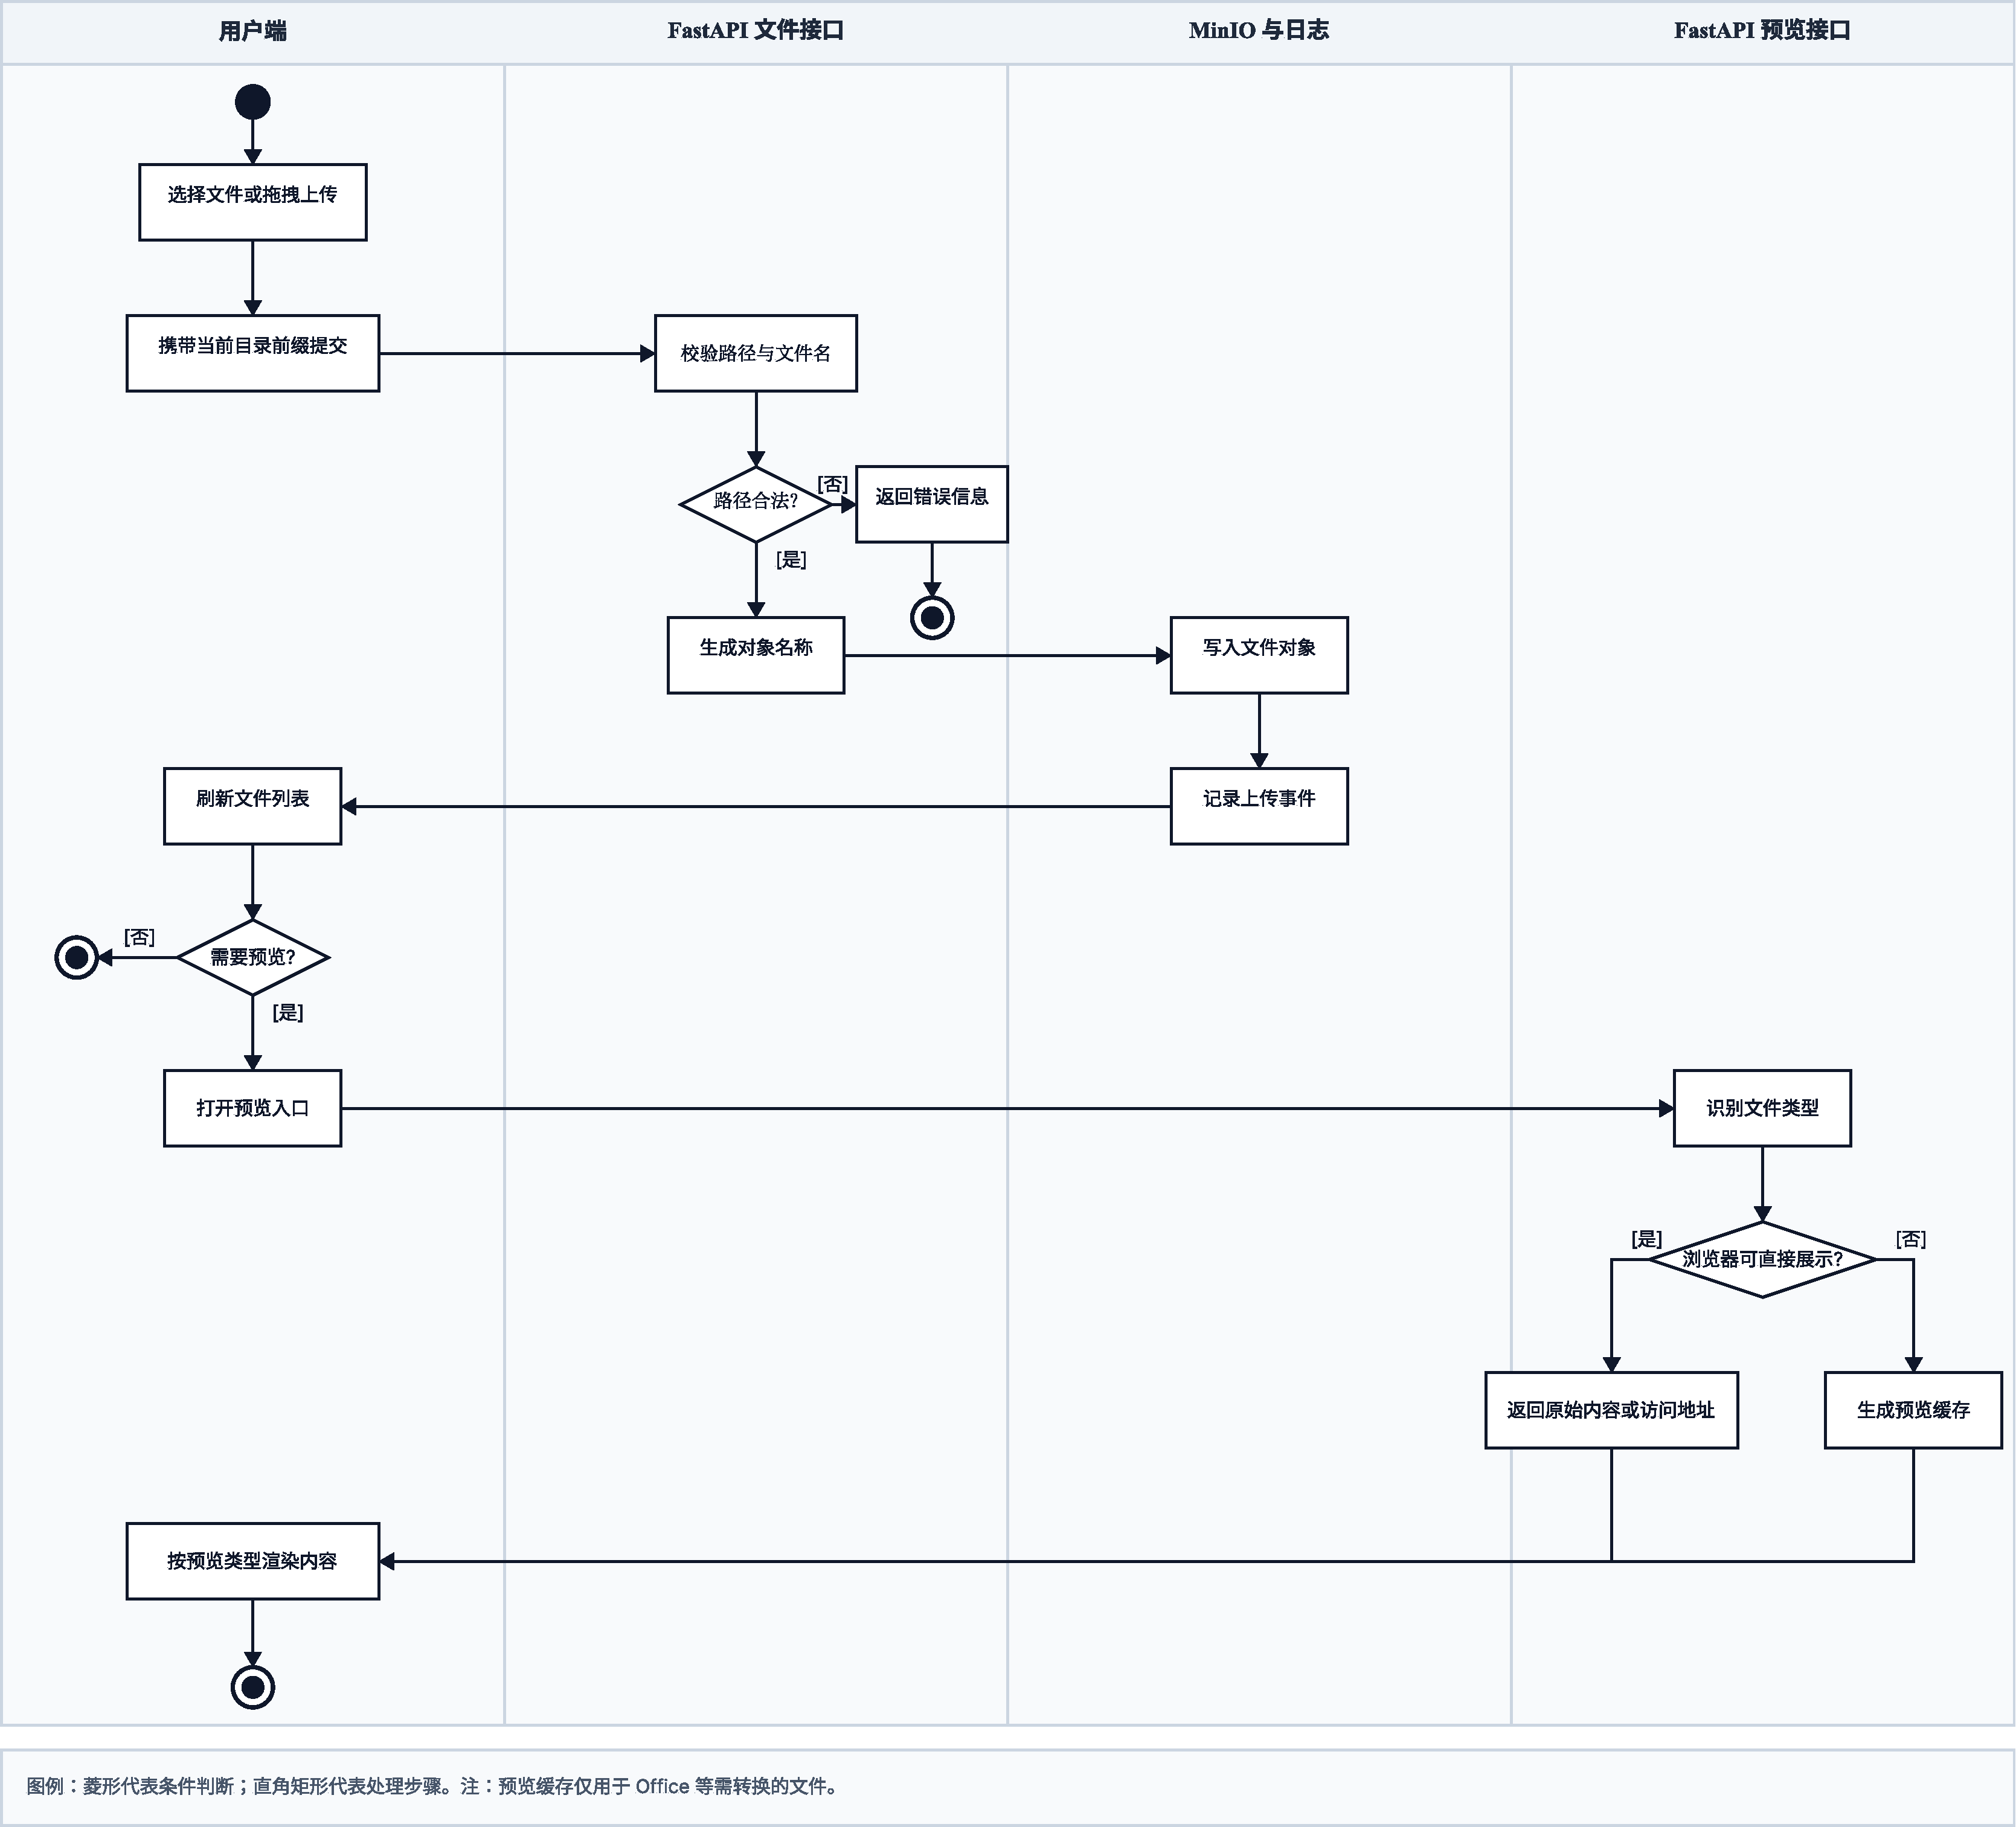
\includegraphics[width=0.92\textwidth,height=0.58\textheight,keepaspectratio]{figures-pdf/fig10-文件预览活动图.pdf}
  \caption{文件上传、整理与预览活动图}
  \label{fig:chap04-preview-flow}
\end{figure}

\subsection{格式转换流程}

格式转换采用“提交任务、后台处理、短轮询读取状态”的异步流程。用户在转换中心选择目标格式后，前端调用转换接口；后端首先执行 P0 白名单校验，通过后创建任务标识并写入 Redis，随后使用 FastAPI BackgroundTasks 启动后台转换逻辑。转换任务进入处理中状态后，从 MinIO 读取源文件，调用 Gotenberg 或本地转换库生成结果，最终将产物写回 \texttt{conversions/} 前缀并更新任务状态。前端通过任务查询接口读取状态、错误信息和结果地址。图 \ref{fig:chap04-conversion-sequence} 展示了该时序。

该流程的设计重点有三点。第一，转换能力必须先经过白名单过滤，防止页面上未开放的实验能力被直接提交到后端执行。第二，转换结果统一通过后端文件内容接口代理下载，而不是把对象存储内部地址直接暴露给浏览器。第三，任务状态与日志事件同步写入，使“转换完成”“转换失败”“结果可下载”三个判断来自同一后端事实，而不是分别由前端按钮状态推断。

\begin{figure}[H]
  \centering
  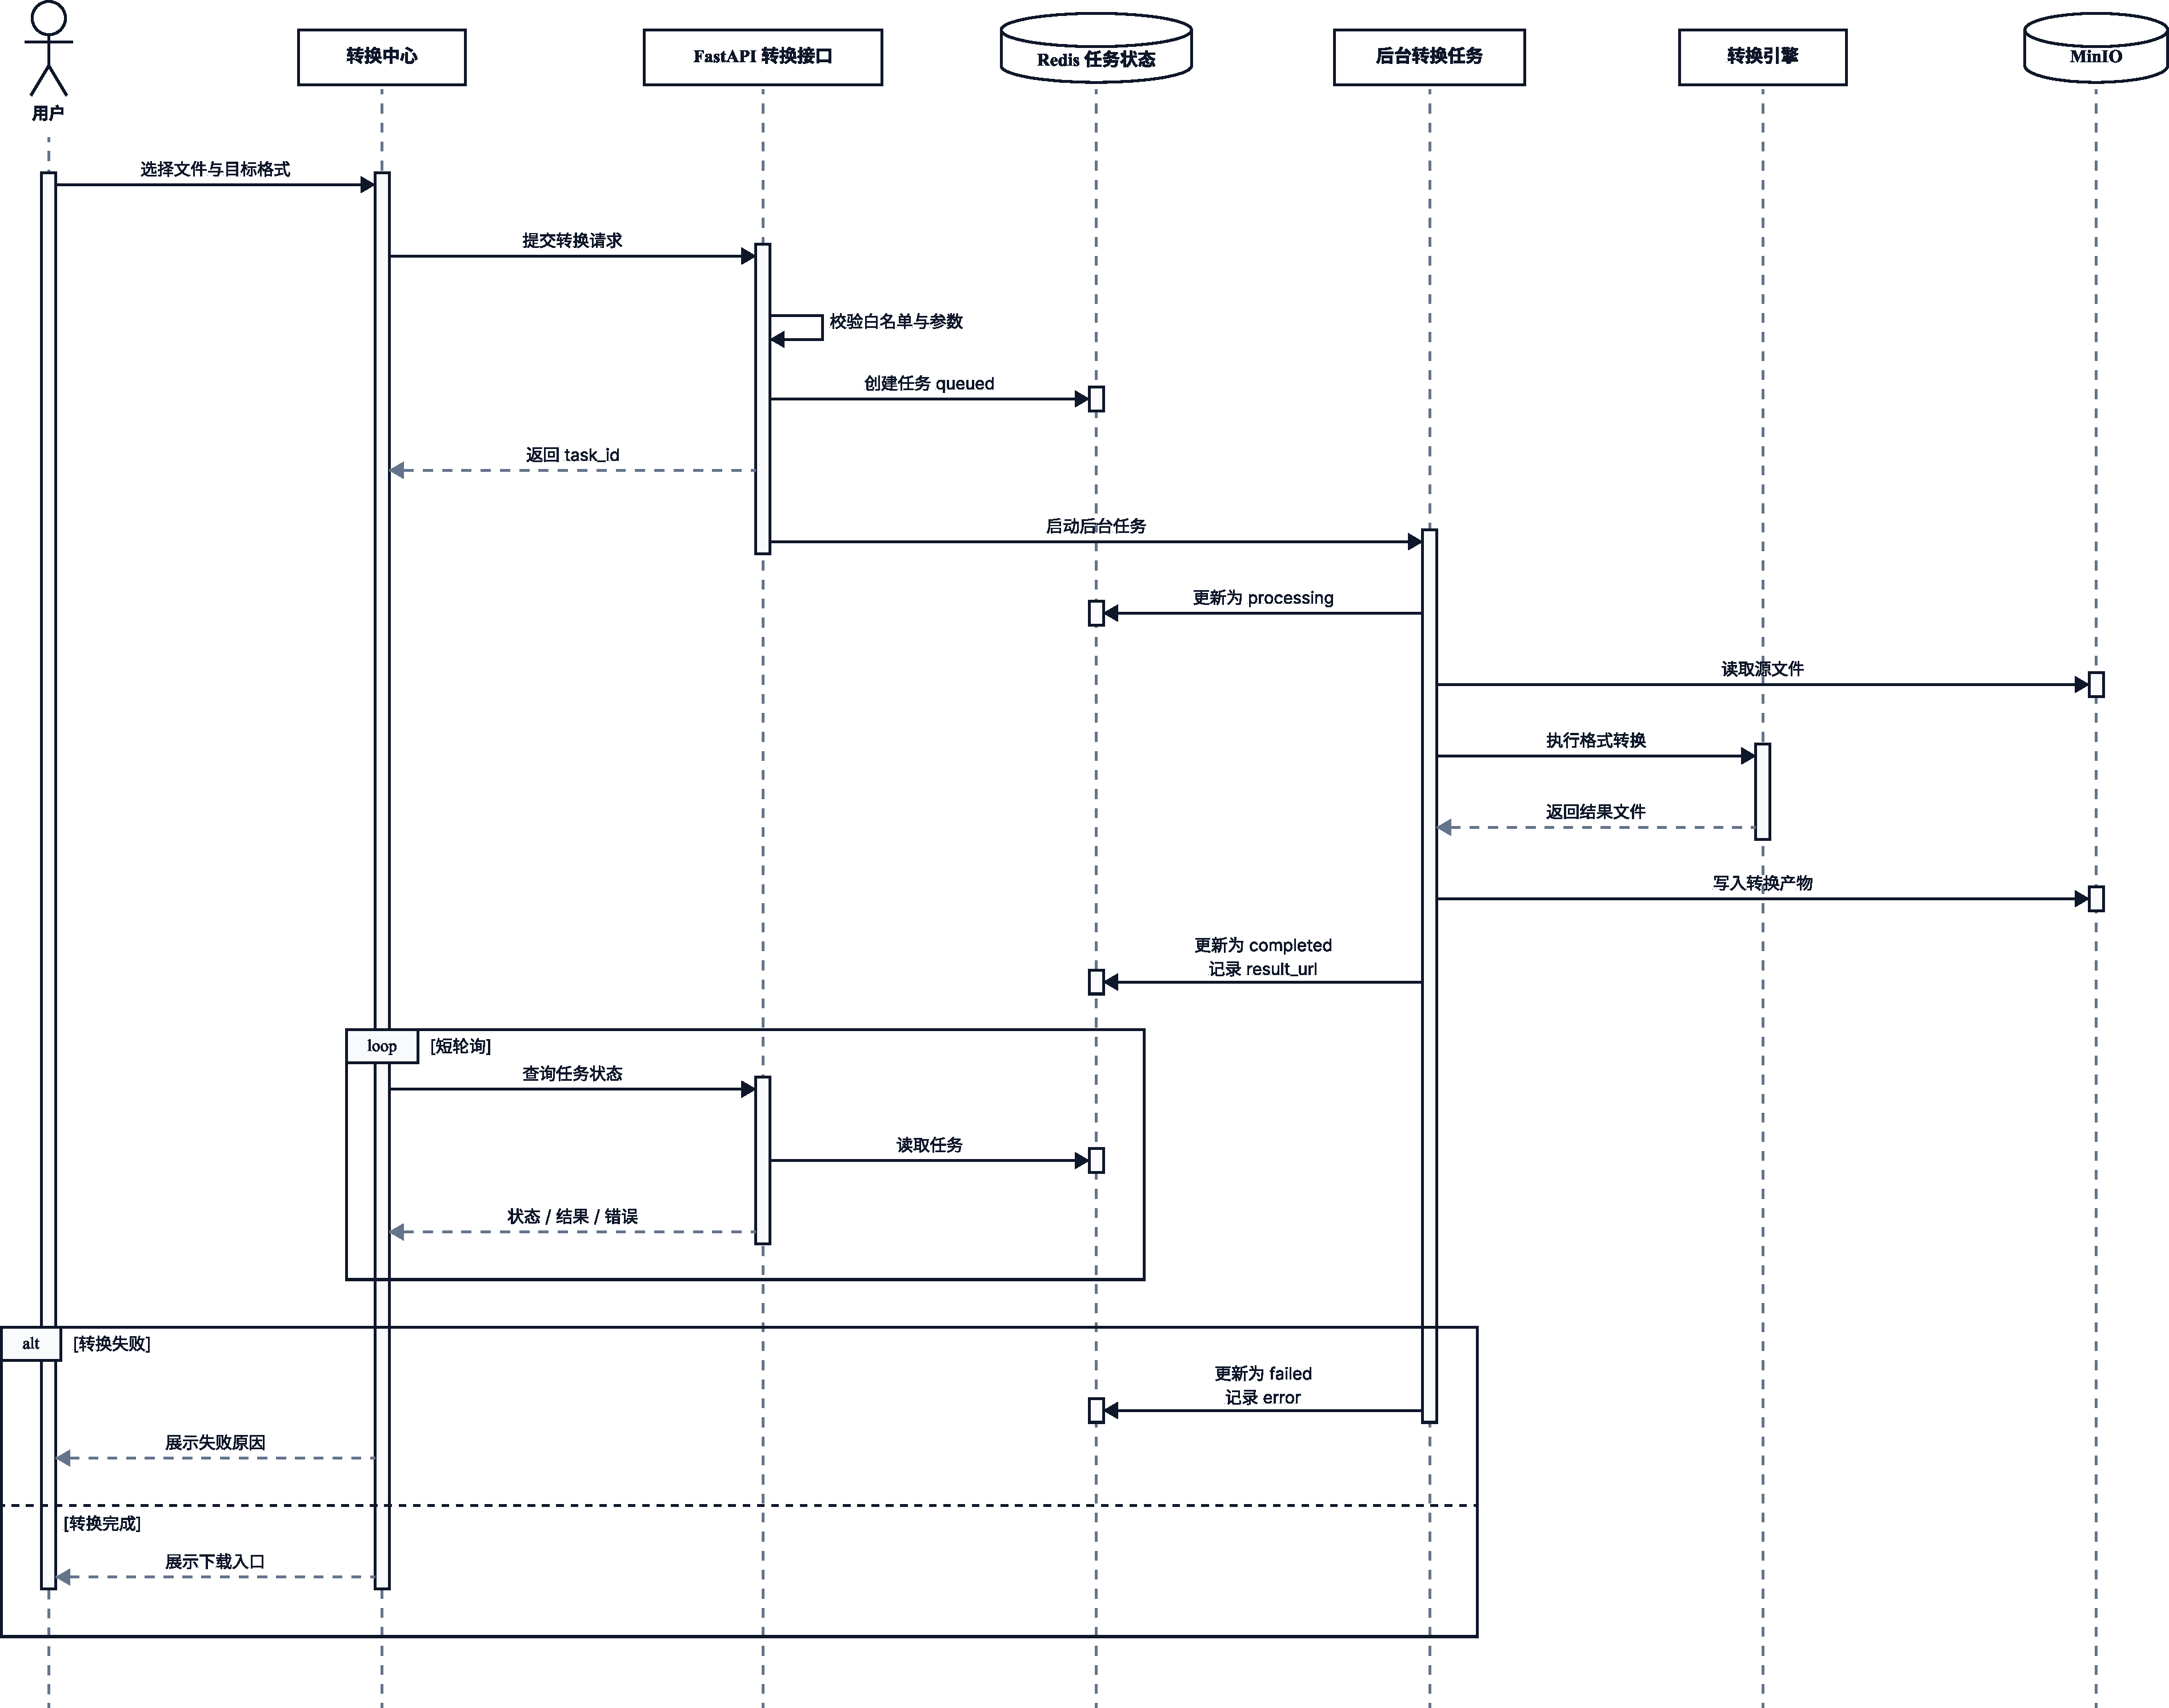
\includegraphics[width=0.96\textwidth,height=0.55\textheight,keepaspectratio]{figures-pdf/fig11-格式转换任务时序图.pdf}
  \caption{格式转换任务时序图}
  \label{fig:chap04-conversion-sequence}
\end{figure}

\subsection{PDF 编辑与导出流程}

PDF 编辑室将原始 PDF 拆解为页面图像，并在前端维护页面顺序、旋转角度、删除状态和批注对象。用户提交导出时，前端把页面配置传给 \texttt{/api/v1/convert/pdf/process}，后端根据配置重新组装 PDF 页面并写入批注，生成的新文件保存到 MinIO。该流程的关键设计是将“页面操作状态”与“最终 PDF 产物”分离：前端负责交互和坐标记录，后端负责文件级重组与输出。图 \ref{fig:chap04-pdf-flow} 展示了 PDF 编辑与导出流程。

\begin{figure}[H]
  \centering
  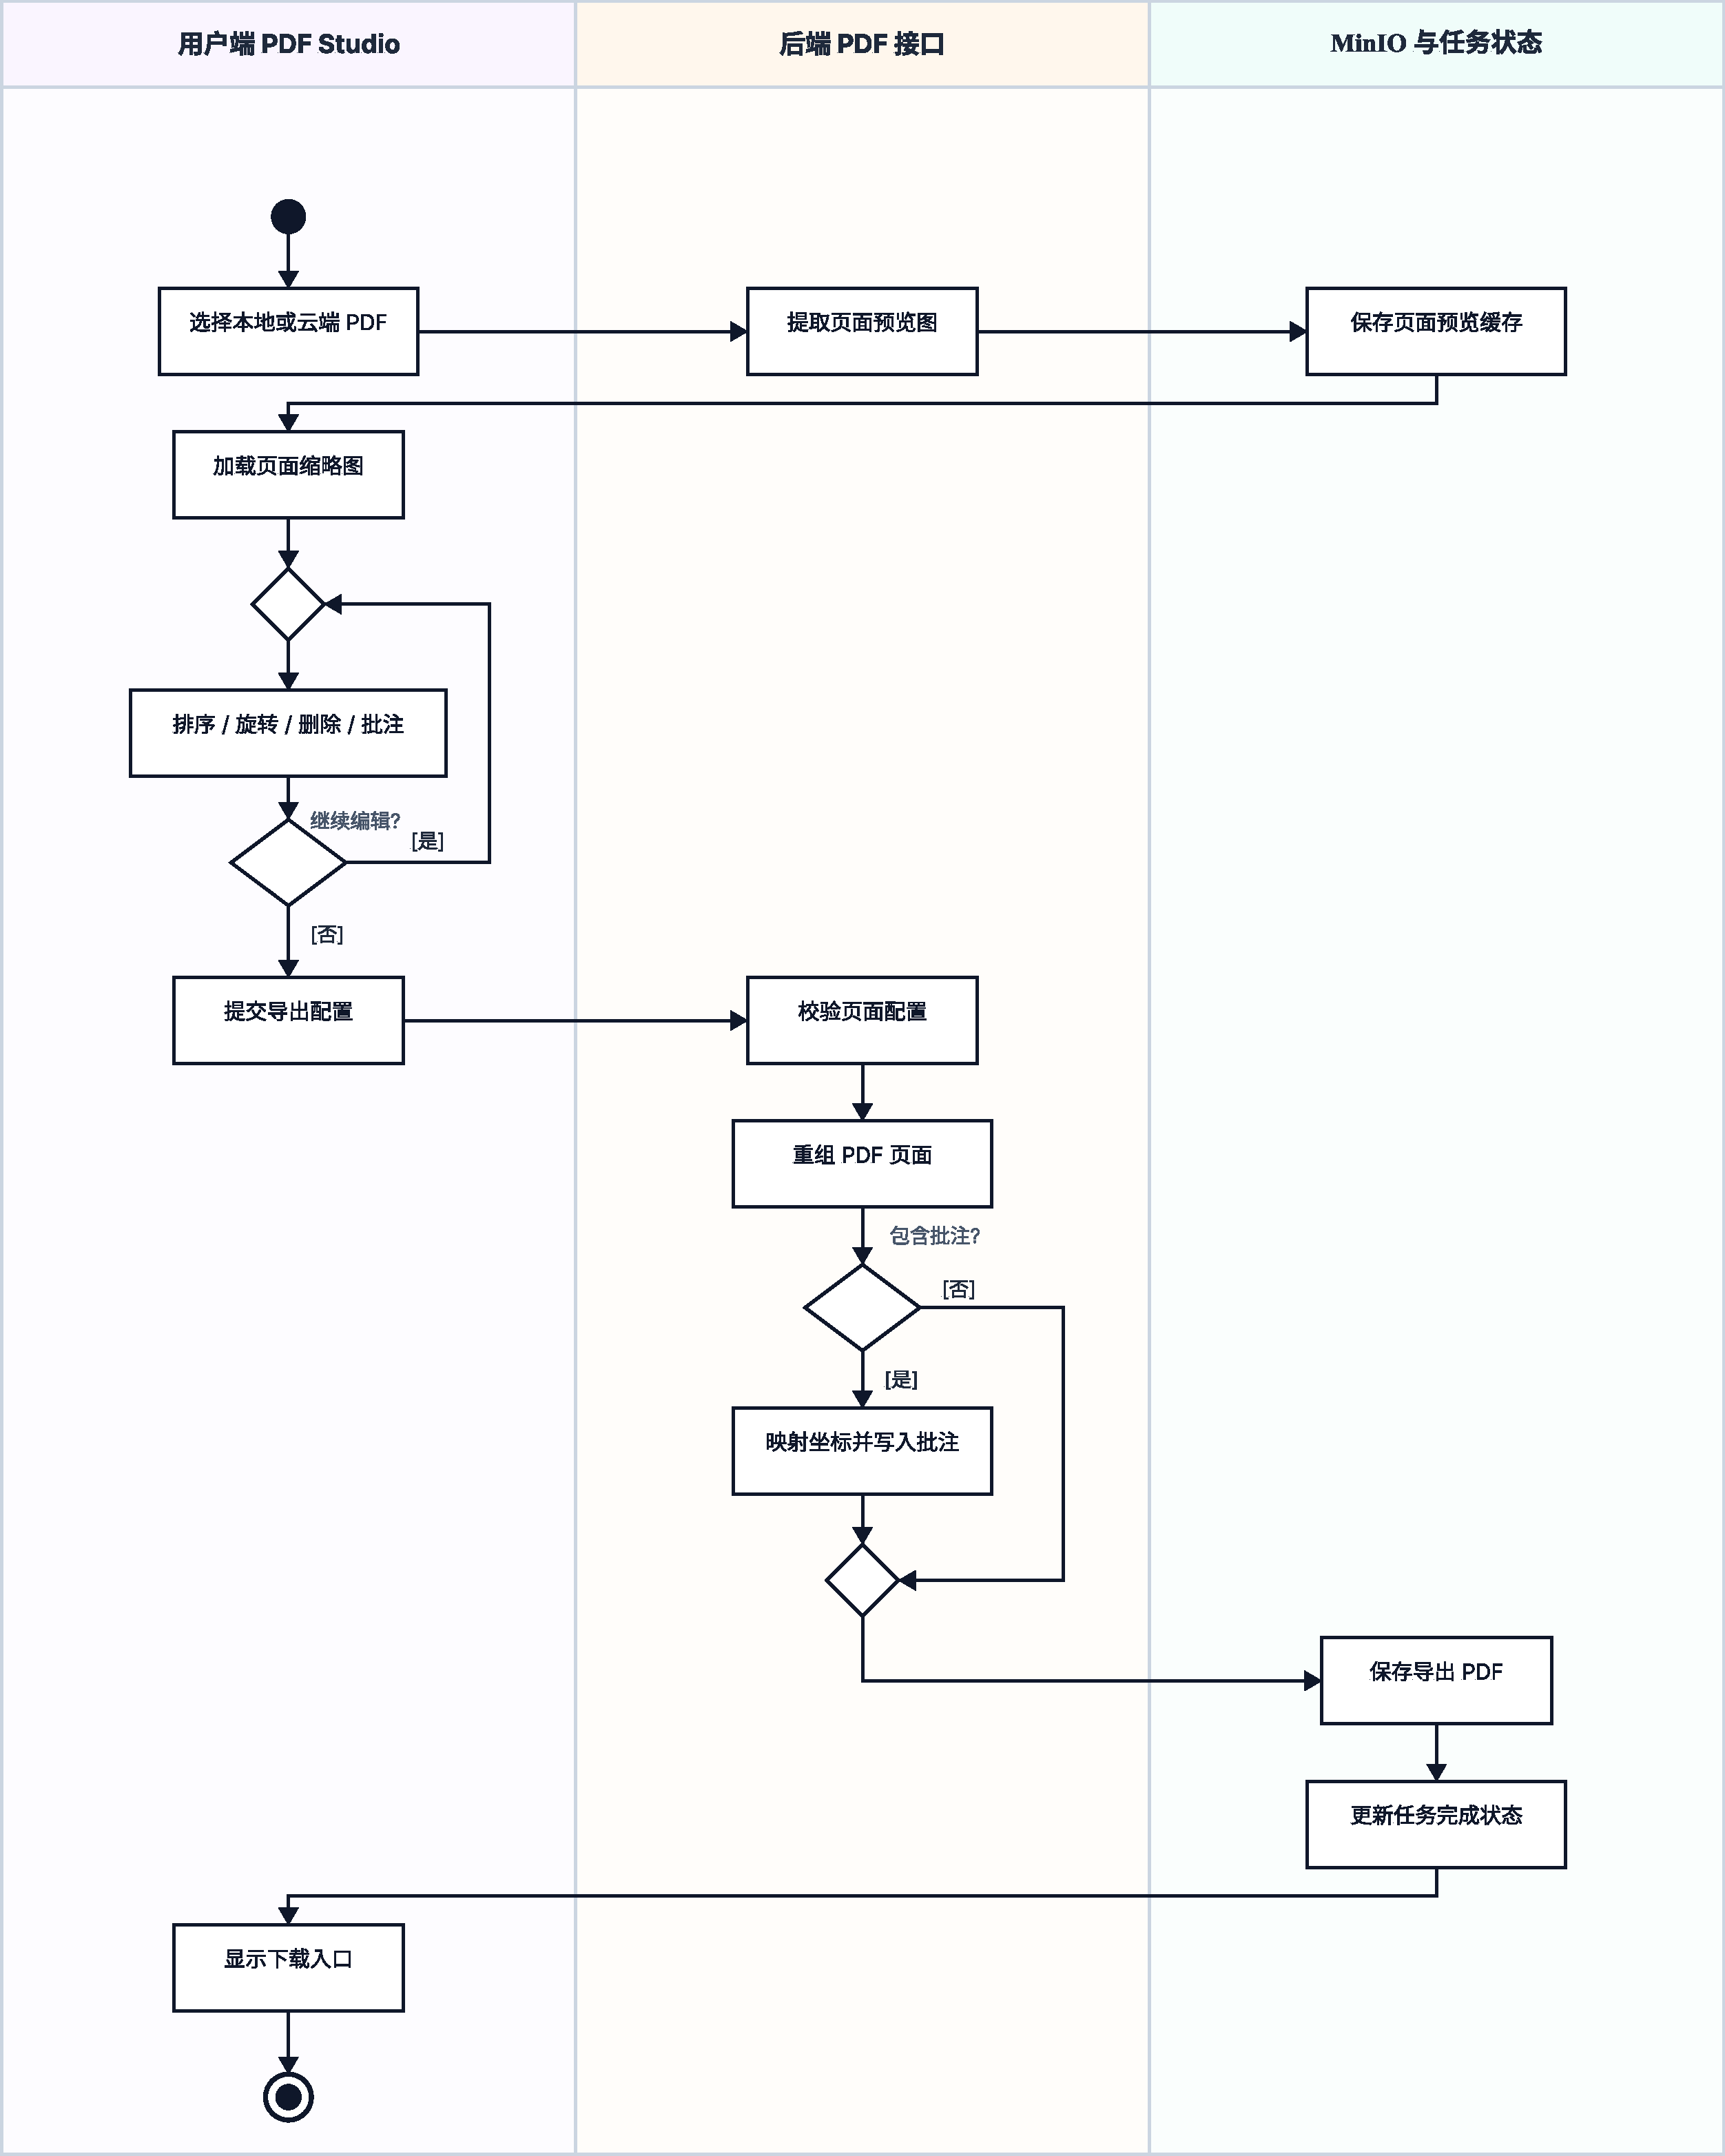
\includegraphics[width=0.90\textwidth,height=0.55\textheight,keepaspectratio]{figures-pdf/fig12-pdf编辑和批注导出活动图.pdf}
  \caption{PDF 编辑室页面整理与导出活动图}
  \label{fig:chap04-pdf-flow}
\end{figure}

\section{核心算法设计}

\subsection{预览类型分派算法}

文件预览需要在多种格式之间做稳定分派。设计上，前端不直接解析所有文件，而是由后端根据对象名和扩展名返回预览类型、内容地址和可预览状态。算法 \ref{alg:preview-dispatch} 给出了预览分派规则。该算法把二进制直读、文本结构化渲染、Office 预览缓存和不可预览状态区分开，便于第 5 章在 \texttt{preview.py} 与 \texttt{services/preview.py} 中落地。

\begin{algorithm}[H]
  \caption{文件预览类型分派算法}
  \label{alg:preview-dispatch}
  \renewcommand{\algorithmicrequire}{\textbf{输入：}}
  \renewcommand{\algorithmicensure}{\textbf{输出：}}
  \begin{algorithmic}[1]
    \Require 文件对象名 $objectName$，文件扩展名 $ext$
    \Ensure 预览类型 $previewType$ 与内容地址 $contentUrl$
    \If{$ext$ 属于 PDF、图片、音频或视频}
      \State 返回后端内容代理地址
    \ElsIf{$ext$ 属于 TXT、Markdown 或 CSV}
      \State 读取对象内容并生成结构化响应
    \ElsIf{$ext$ 属于 Office 文档}
      \State 查询或生成 PDF 预览缓存
    \Else
      \State 返回不可预览状态和下载入口
    \EndIf
  \end{algorithmic}
\end{algorithm}

\subsection{异步任务状态算法}

格式转换和 PDF 导出均属于耗时文件处理任务。系统采用“先建任务、后处理文件、再更新终态”的设计，避免用户请求长时间阻塞。算法 \ref{alg:async-task-process} 给出了异步处理的统一状态更新规则。任务必须经历等待、处理中、成功或失败状态，成功路径需要写入对象产物和结果地址，失败路径需要写入错误原因。

\begin{algorithm}[H]
  \caption{异步文件处理任务状态更新算法}
  \label{alg:async-task-process}
  \renewcommand{\algorithmicrequire}{\textbf{输入：}}
  \renewcommand{\algorithmicensure}{\textbf{输出：}}
  \begin{algorithmic}[1]
    \Require 任务编号 $taskId$，输入文件 $file$，处理类型 $kind$
    \Ensure 任务终态、结果地址或错误信息
    \State 写入任务状态 $pending$
    \State 后台任务启动，写入任务状态 $processing$
    \State 记录开始事件到运行日志
    \If{$kind$ 为格式转换}
      \State 按白名单选择转换方法并生成结果字节
    \Else
      \State 按页面配置重组 PDF 页面与批注
    \EndIf
    \If{处理成功}
      \State 将结果写入 MinIO 的 \texttt{conversions/} 前缀
      \State 写入任务状态 $success$ 与 API 代理结果地址
      \State 记录完成事件到运行日志
    \Else
      \State 写入任务状态 $failed$ 与错误原因
      \State 记录失败事件到运行日志
    \EndIf
  \end{algorithmic}
\end{algorithm}

前端轮询以任务终态作为停止边界。设第 $k$ 次查询到的任务状态为 $s_k$，终态集合为 $\Omega=\{success,failed\}$，则轮询停止条件为：
\begin{equation}
  s_k \in \Omega.
  \label{eq:polling-stop}
\end{equation}
式 \ref{eq:polling-stop} 可避免任务已完成后仍持续请求后端。

\subsection{PDF 页面导出算法}

PDF 编辑室的导出需要把前端页面顺序、旋转角度、删除状态和批注对象转化为后端可写入的 PDF 产物。批注导出的关键是坐标映射。设前端画布坐标为 $(x_c,y_c)$，画布宽高为 $W_c,H_c$，PDF 页面宽高为 $W_p,H_p$，则写回 PDF 时的坐标可表示为：
\begin{equation}
  x_p=x_c\cdot\frac{W_p}{W_c},\qquad
  y_p=y_c\cdot\frac{H_p}{H_c}.
  \label{eq:pdf-coordinate-map}
\end{equation}
式 \ref{eq:pdf-coordinate-map} 说明批注位置应由画布尺寸与 PDF 页面尺寸之间的比例确定，而不是依赖浏览器缩放值。

\begin{algorithm}[H]
  \caption{PDF 页面重组与批注导出算法}
  \label{alg:pdf-export}
  \renewcommand{\algorithmicrequire}{\textbf{输入：}}
  \renewcommand{\algorithmicensure}{\textbf{输出：}}
  \begin{algorithmic}[1]
    \Require 页面配置数组 $pages$，输出文件名 $name$
    \Ensure 导出 PDF 对象地址
    \State 清洗输出文件名并创建任务编号
    \For{每个页面配置 $page$}
      \State 读取源 PDF 页面并应用旋转与顺序
      \State 按式 \ref{eq:pdf-coordinate-map} 换算批注坐标
      \State 将文本、画笔、矩形和箭头写入页面
    \EndFor
    \State 合并页面并写入 MinIO
    \State 返回 API 代理下载地址
  \end{algorithmic}
\end{algorithm}

\section{数据结构设计}

\subsection{MinIO 对象结构}

系统将 MinIO 作为文件对象的统一存储位置。用户上传的原始文件以对象名保存，文件夹通过路径前缀和 \texttt{.keep} 空对象表达；预览缓存保存到 \texttt{previews/} 前缀；转换结果与 PDF 导出结果保存到 \texttt{conversions/} 前缀。对象名不仅是存储键，也是前端目录和文件定位的主要依据，因此上传、移动、重命名和删除接口都必须维护对象名前缀的一致性。

对象存储占用沿用第 3 章式 \ref{eq:req-storage-size} 的需求口径。总体设计阶段需要进一步明确对象集合的过滤规则：用户容量统计只聚合原始文件对象和用户可见产物，不把目录占位对象、预览缓存和转换中间文件混入容量展示。这样能够避免文件夹数量或预览次数影响用户对真实资料规模的判断。

\subsection{Redis 状态结构}

Redis 承担两类状态：一类是任务状态，包含任务标识、任务类型、当前状态、结果地址、错误信息和时间戳；另一类是事件日志和健康快照，用于管理端观察近期操作和服务状态。任务状态至少覆盖 \texttt{pending}、\texttt{processing}、\texttt{success} 和 \texttt{failed}，事件日志按时间线保存上传、预览、转换、PDF 导出和系统健康相关事件。第 3 章图 \ref{fig:chap03-er-model} 已概括 MinIO 与 Redis 的概念数据模型，本节进一步说明状态存储设计。

任务总量沿用第 3 章式 \ref{eq:req-task-total} 的需求口径。Redis 设计需要保证等待、处理中、成功和失败任务能够被独立统计，并且任务总量只来自当前业务任务集合，避免与 Spark 历史样本规模混淆。

任务状态从创建到终态存在明确的迁移约束。转换任务与 PDF 页面处理任务提交后先进入等待状态，后台任务启动后进入处理中状态，产物写入 MinIO 后进入成功状态，异常捕获后进入失败状态。状态变化同时触发事件日志写入，使任务监控、运行拓扑和近期事件列表能够读取同一条业务链路。图 \ref{fig:chap04-task-state-flow} 描述了状态迁移与事件传播关系。

\begin{figure}[H]
  \centering
  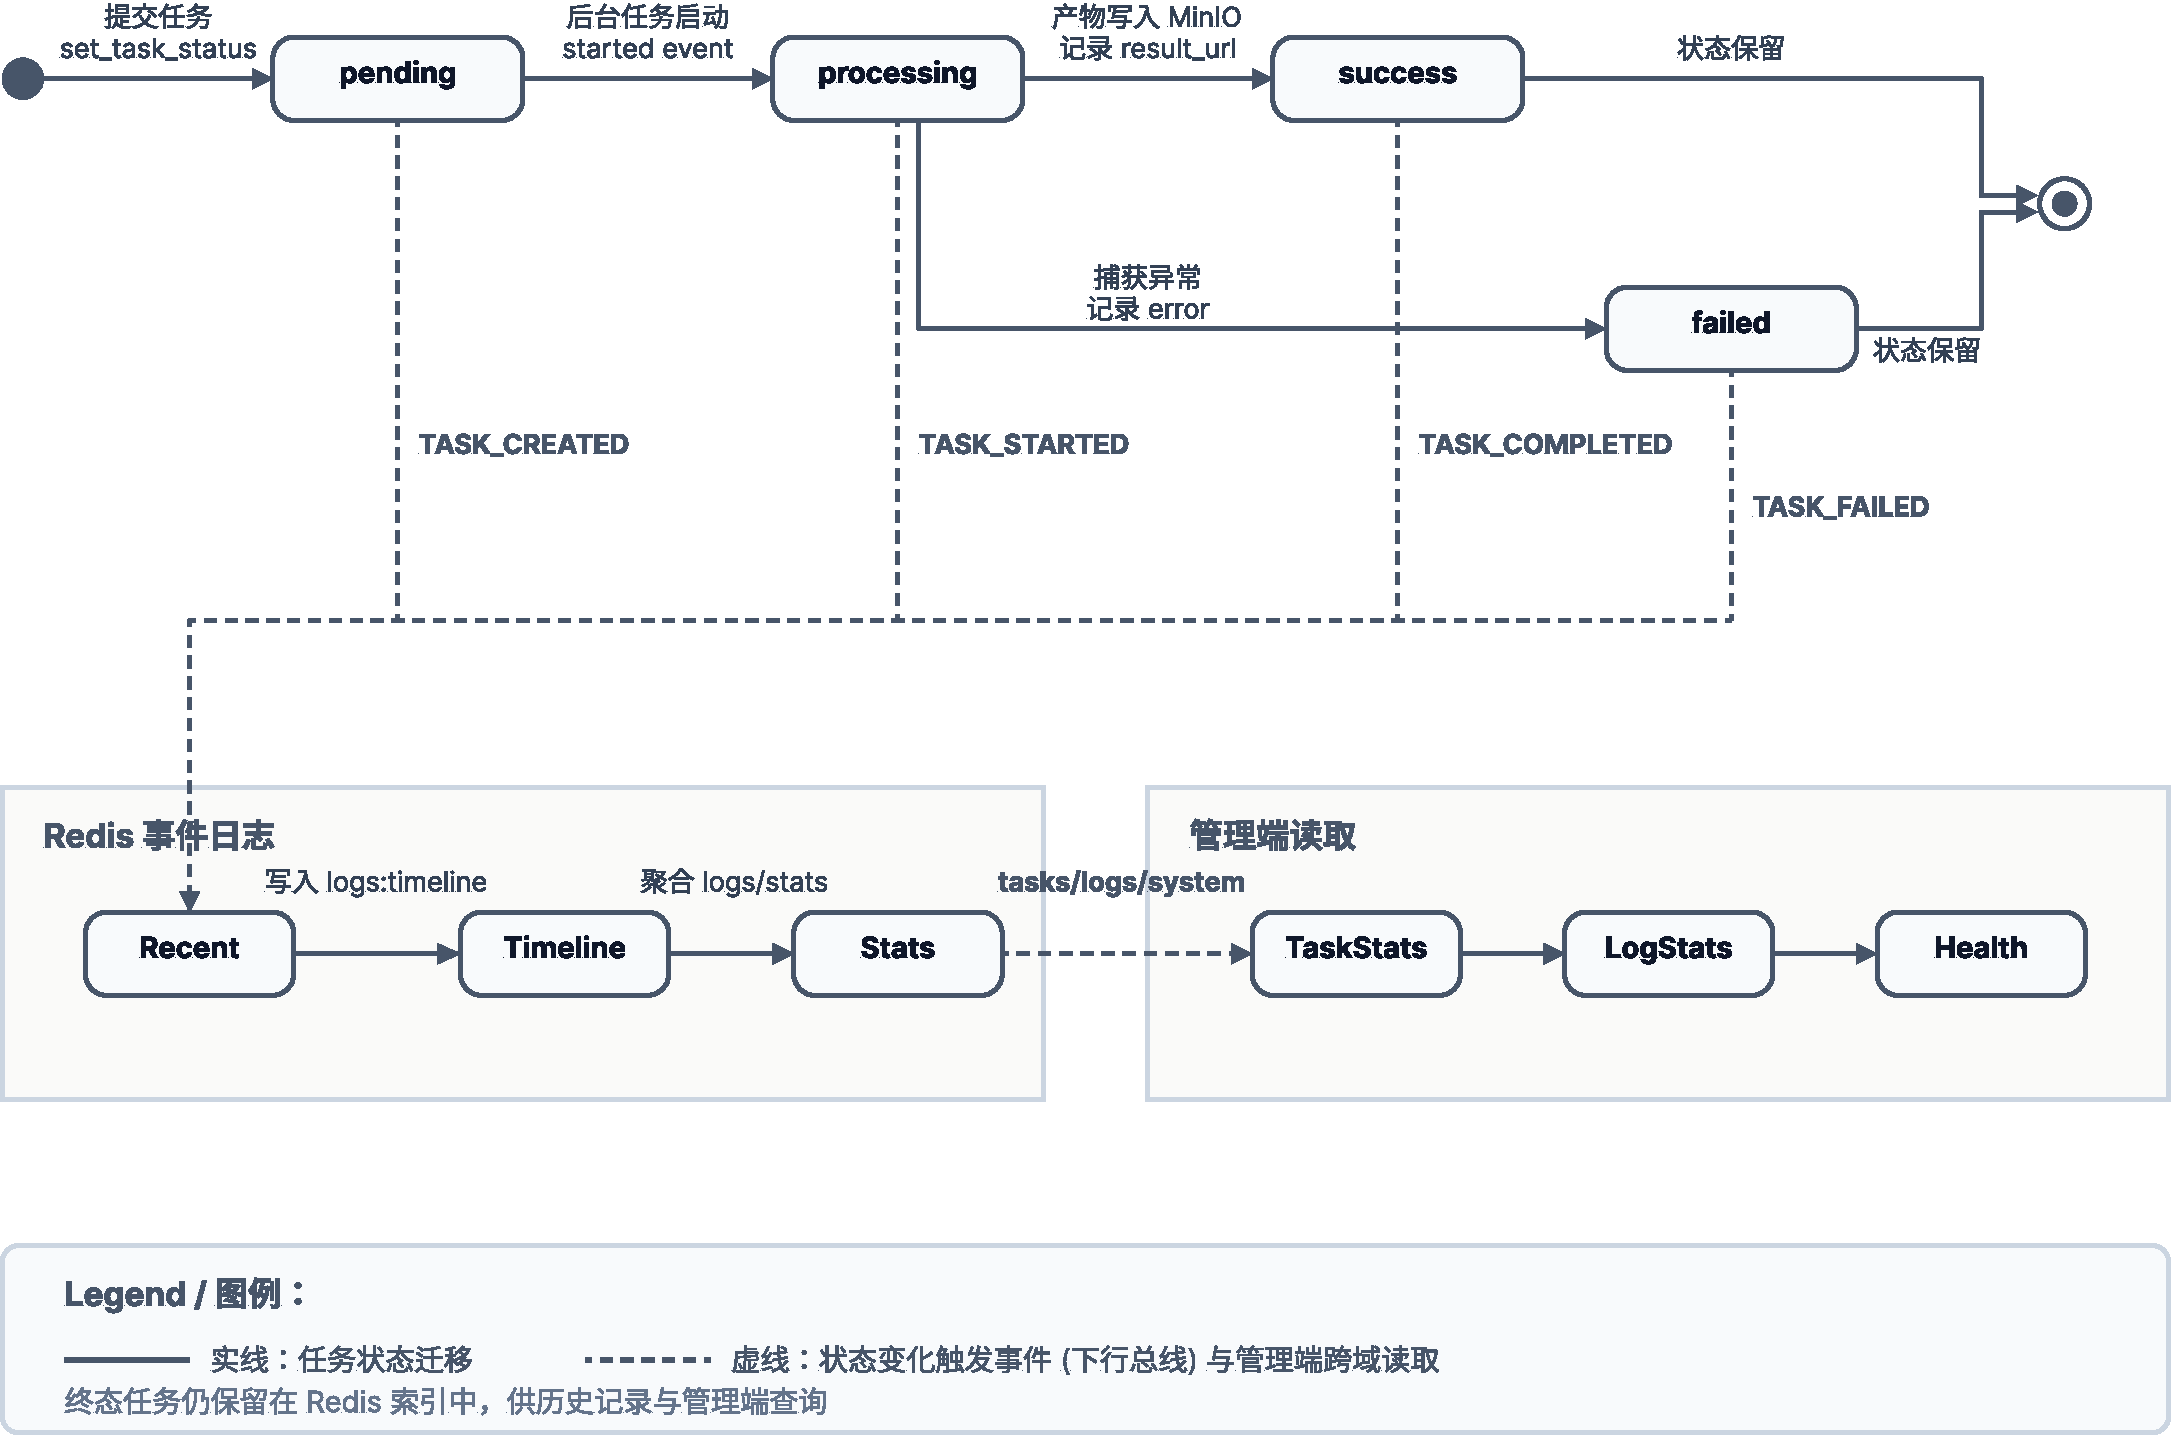
\includegraphics[width=0.92\textwidth,height=0.50\textheight,keepaspectratio]{figures-pdf/fig17-任务状态与事件流转图.pdf}
  \caption{任务状态与事件流转图}
  \label{fig:chap04-task-state-flow}
\end{figure}

\section{管理驾驶舱数据管线设计}

管理驾驶舱采用实时运行数据与历史分析样本并行的设计。实时运行数据直接来自 FastAPI 接口，适合反映当前文件数、任务数、失败数、队列长度、近期事件和服务健康；历史分析样本来自 Spark 输出，适合表达较长窗口下的文件类型分布、转换矩阵、趋势变化和质量分析。图 \ref{fig:chap04-analytics-pipeline} 展示了这一管线。该设计使用户端操作能够进入实时观察，同时保留大数据课程场景下的离线分析能力。

实时运行指标的计算以 Redis 中的任务集合与日志统计为基础。在式 \ref{eq:req-task-total} 的基础上，管理端第一屏的任务成功率与失败占比定义为：
\begin{equation}
  R_s=\frac{C}{\max(T,1)},\qquad
  R_f=\frac{F}{\max(T,1)}.
  \label{eq:task-rate}
\end{equation}
其中 $R_s$ 表示任务成功率，$R_f$ 表示失败占比，分母使用 $\max(T,1)$ 是为了避免任务总量为零时产生无意义除法。近 24 小时事件规模直接来自日志统计，记为 $L_{24}=E_{24}$。式 \ref{eq:task-rate} 对应前端读取的 \texttt{/api/v1/tasks/stats}、\texttt{/api/v1/tasks/queue-length} 与 \texttt{/api/v1/logs/stats}，用于解释管理端实时数值会随业务操作发生变化。

\begin{figure}[H]
  \centering
  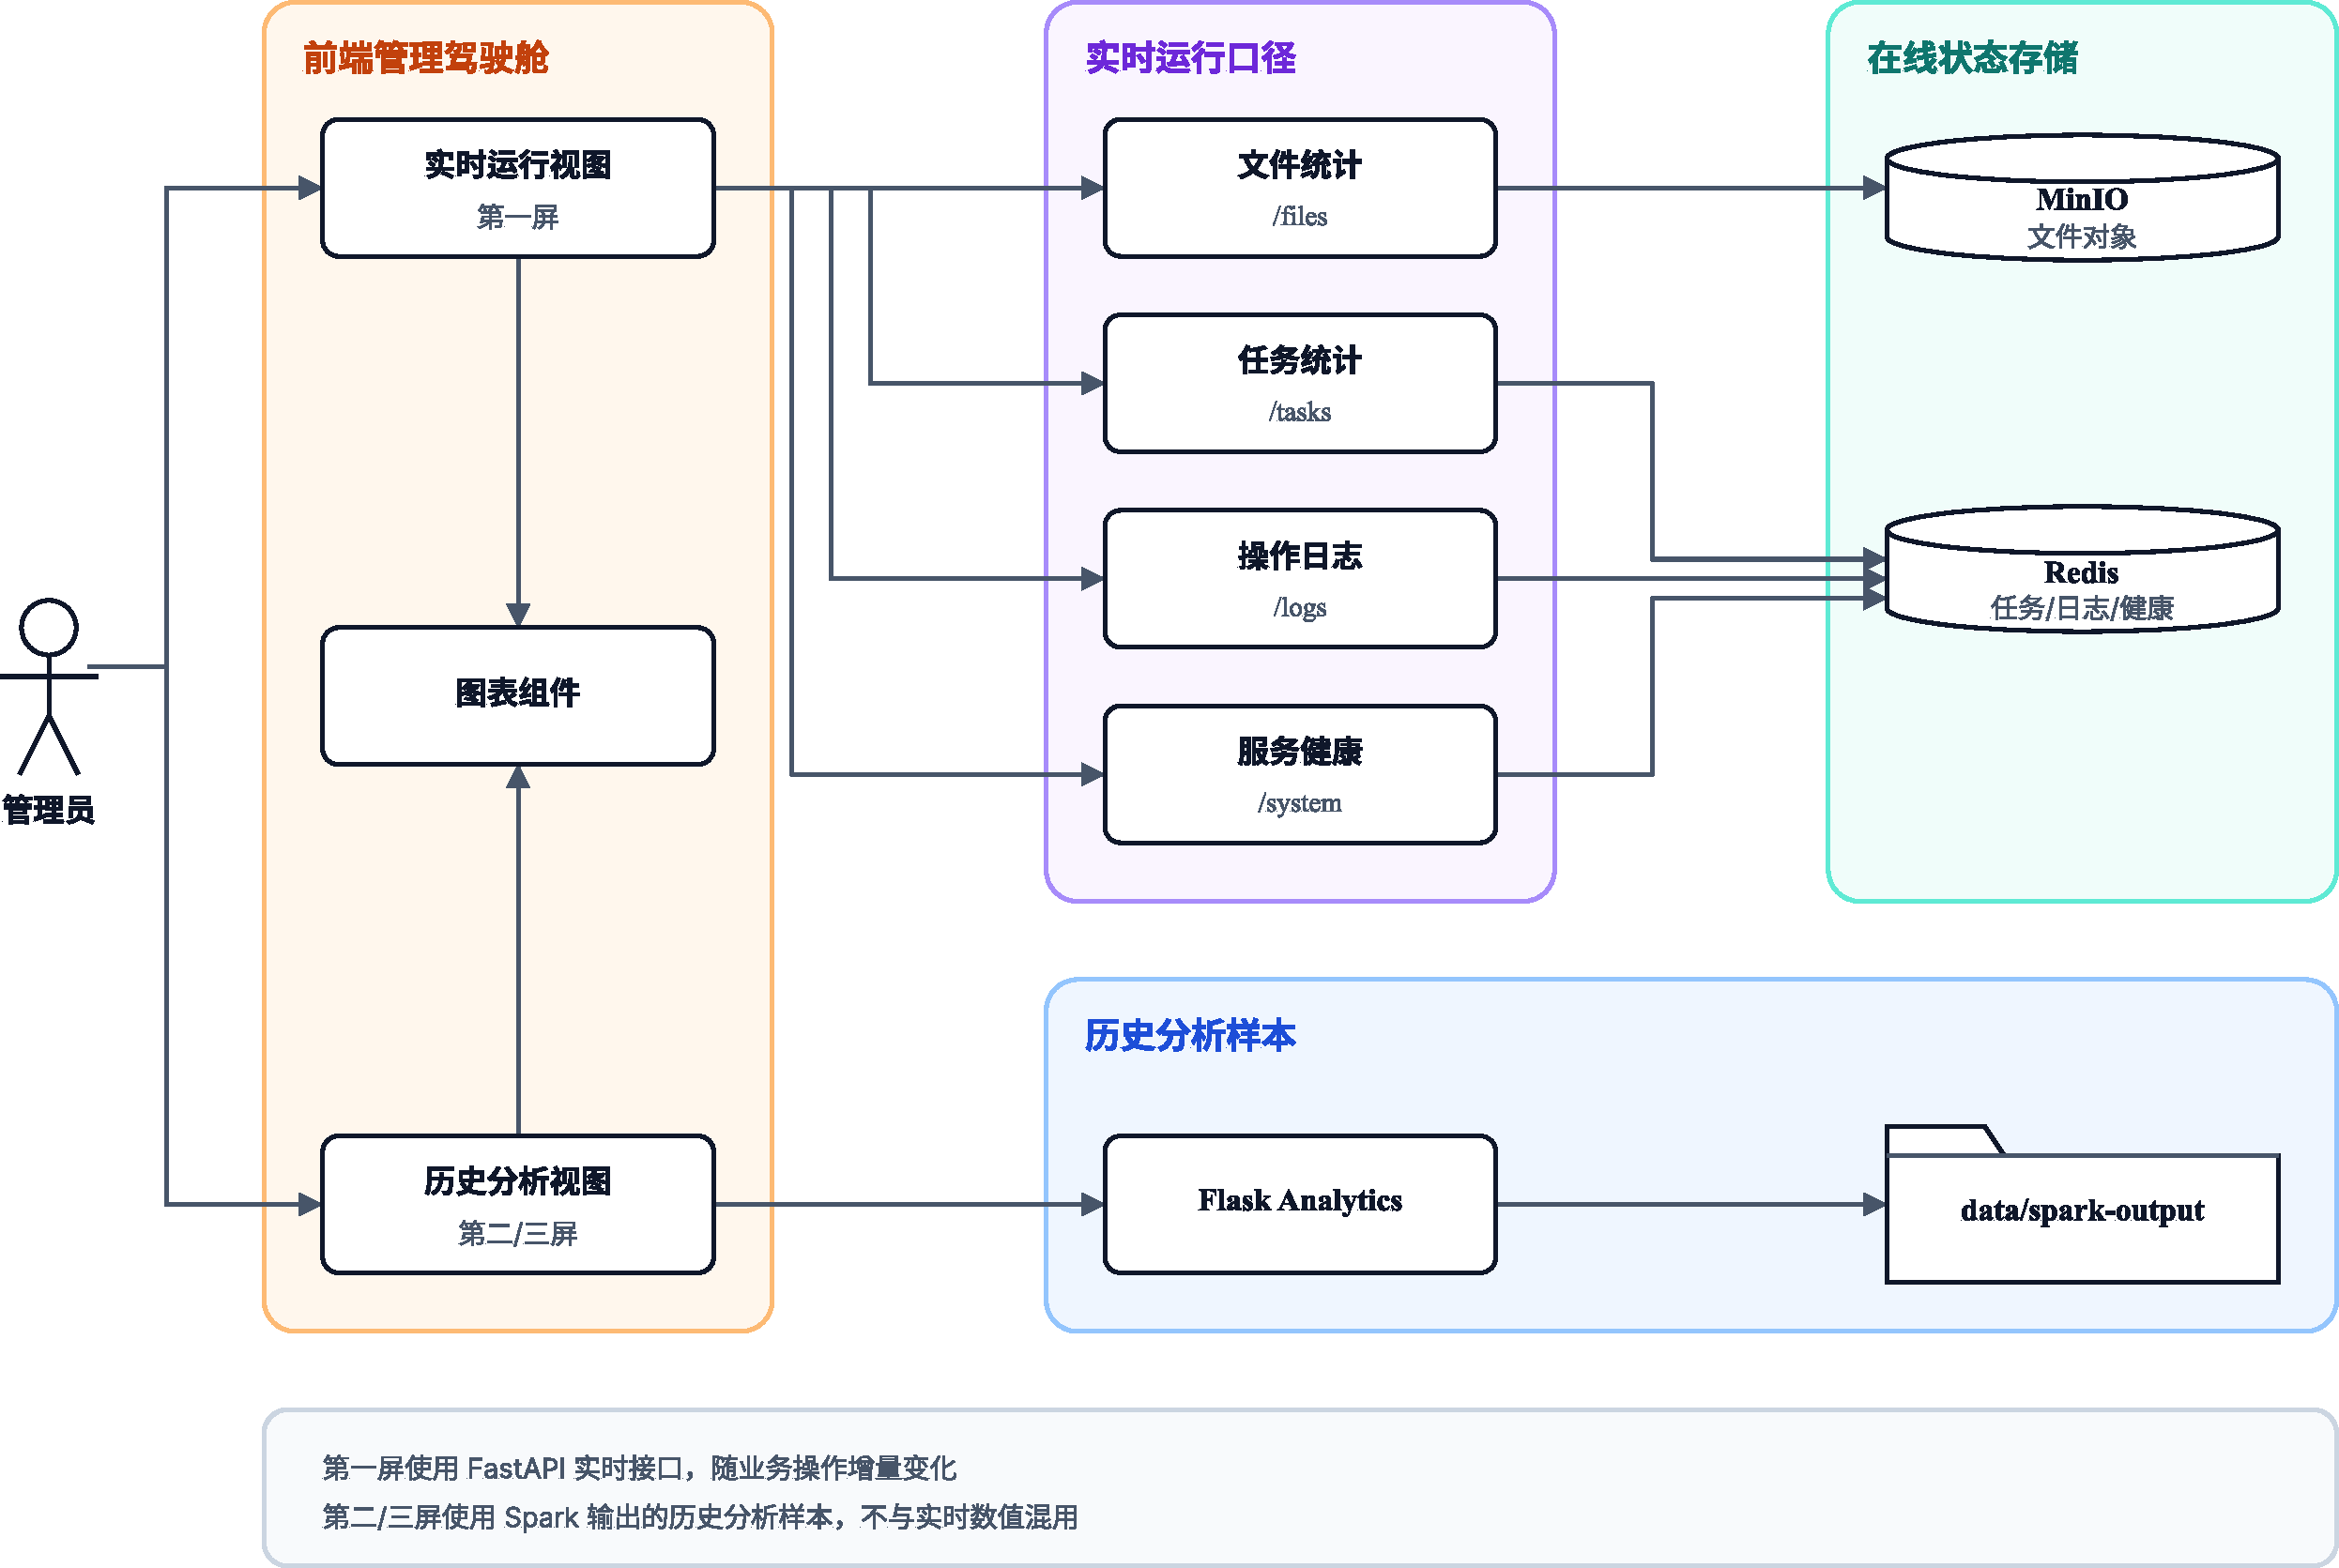
\includegraphics[width=0.96\textwidth,height=0.52\textheight,keepaspectratio]{figures-pdf/fig14-管理驾驶舱数据管线图.pdf}
  \caption{管理驾驶舱数据管线图}
  \label{fig:chap04-analytics-pipeline}
\end{figure}

\section{部署结构设计}

系统采用本地进程管理与容器化基础依赖结合的部署方式。前端开发服务与 Flask 分析服务适合使用 PM2 管理，便于快速重启、查看日志和保留长期运行状态；Redis、MinIO、Gotenberg 等基础依赖适合由 Docker Compose 管理，确保端口、网络和数据卷稳定。FastAPI 主服务启动时初始化 MinIO、Redis 和健康检查循环，保证 API 可用性与基础依赖状态能够被系统状态接口观察到。

从启动顺序看，Redis、MinIO 和 Gotenberg 属于基础依赖，应先于 FastAPI 主服务启动；FastAPI 启动后负责创建存储桶、注册路由和启动健康检查循环；前端与 Flask Analytics 则可以作为独立展示服务由 PM2 持续守护。这样的部署边界使文件处理主链路与历史分析展示链路可以单独重启，降低调试管理端图表时影响用户端上传和转换的概率。

从运行观测看，系统状态接口需要同时覆盖 API、对象存储、任务状态、转换服务和分析服务。若 MinIO 不可用，文件上传和下载会失败；若 Redis 不可用，任务状态和近期事件会失去持久记录；若 Gotenberg 不可用，Office 转 PDF 和部分预览链路会降级。将这些依赖纳入系统状态设计，可以让管理端显示的不只是页面是否打开，而是关键业务能力是否可用。

\section{本章小结}

本章完成了 CulCloud 的系统总体设计，明确了分层架构、模块边界、业务流程、数据结构、运行指标和部署结构。通过业务闭环、任务状态、数据模型和管理管线的组合设计，系统能够把用户端动作转换为可查询任务、可下载产物和可观察指标。

从总体架构看，系统采用前端界面、FastAPI 业务接口、领域服务、对象存储、运行状态和历史分析服务分层组织。该结构的好处是职责边界清晰：前端负责交互和状态展示，FastAPI 负责接口校验和业务编排，MinIO 负责文件对象保存，Redis 负责任务与日志状态，Gotenberg 负责重型文档转换，Spark 与 Flask Analytics 负责历史分析结果读取。不同模块之间通过 API 和对象键建立联系，而不是相互直接读取内部实现。

从业务流程看，本章把上传预览、格式转换、PDF 页面处理和管理端观察放入同一条闭环中分析。文件上传会形成对象和日志，文件预览会形成可复用缓存，转换和 PDF 导出会形成异步任务与结果产物，管理端再读取这些状态形成运行指标。这样的设计使系统不只是多个页面的集合，而是一个可追踪、可解释、可复现的资料处理平台。

从数据和运行角度看，系统没有引入复杂关系数据库，而是利用对象名前缀、任务状态集合和事件日志完成当前阶段所需的数据表达。该选择降低了本地部署和验证成本，但也要求在对象移动、目录删除、预览缓存和转换产物之间保持清晰边界。后续若引入用户权限、共享协作和长期审计，可以在现有对象键和任务标识基础上补充关系索引。

从设计边界看，本章确认的是最小可用平台的总体结构，而不是完整企业级云盘方案。当前设计重点覆盖单用户资料管理、轻量文件处理、异步任务可追踪和管理端观察；对于细粒度权限、多人协同编辑、跨设备同步冲突、对象版本回滚和长期归档策略，只保留可扩展位置。这样能够让系统在课程实践规模内保持可运行、可说明，同时为后续增强留下清晰方向。

因此，第 4 章承担的是“把系统如何组织起来”讲清楚的任务，而不是替代后续实现说明。

下一章将在本章设计基础上进一步落到代码实现，说明各前端视图、API 客户端、后端路由、领域服务和数据对象之间如何协作；第 6 章则从功能用例、命令行结果和业务闭环三个层面验证这些设计是否真正落地。

\chapter{系统详细设计及实现}

本章从代码实现角度说明 CulCloud 的核心模块。系统前端主要位于 \texttt{file-cloud-frontend/src/views/}，统一 API 调用位于 \texttt{file-cloud-frontend/src/services/api.ts}；后端主入口位于 \texttt{backend/app/main.py}，业务路由位于 \texttt{backend/app/routers/}，领域服务位于 \texttt{backend/app/services/}。图 \ref{fig:chap05-component-design} 给出了详细设计组件协作关系，为后续模块说明提供总览。

\begin{figure}[H]
  \centering
  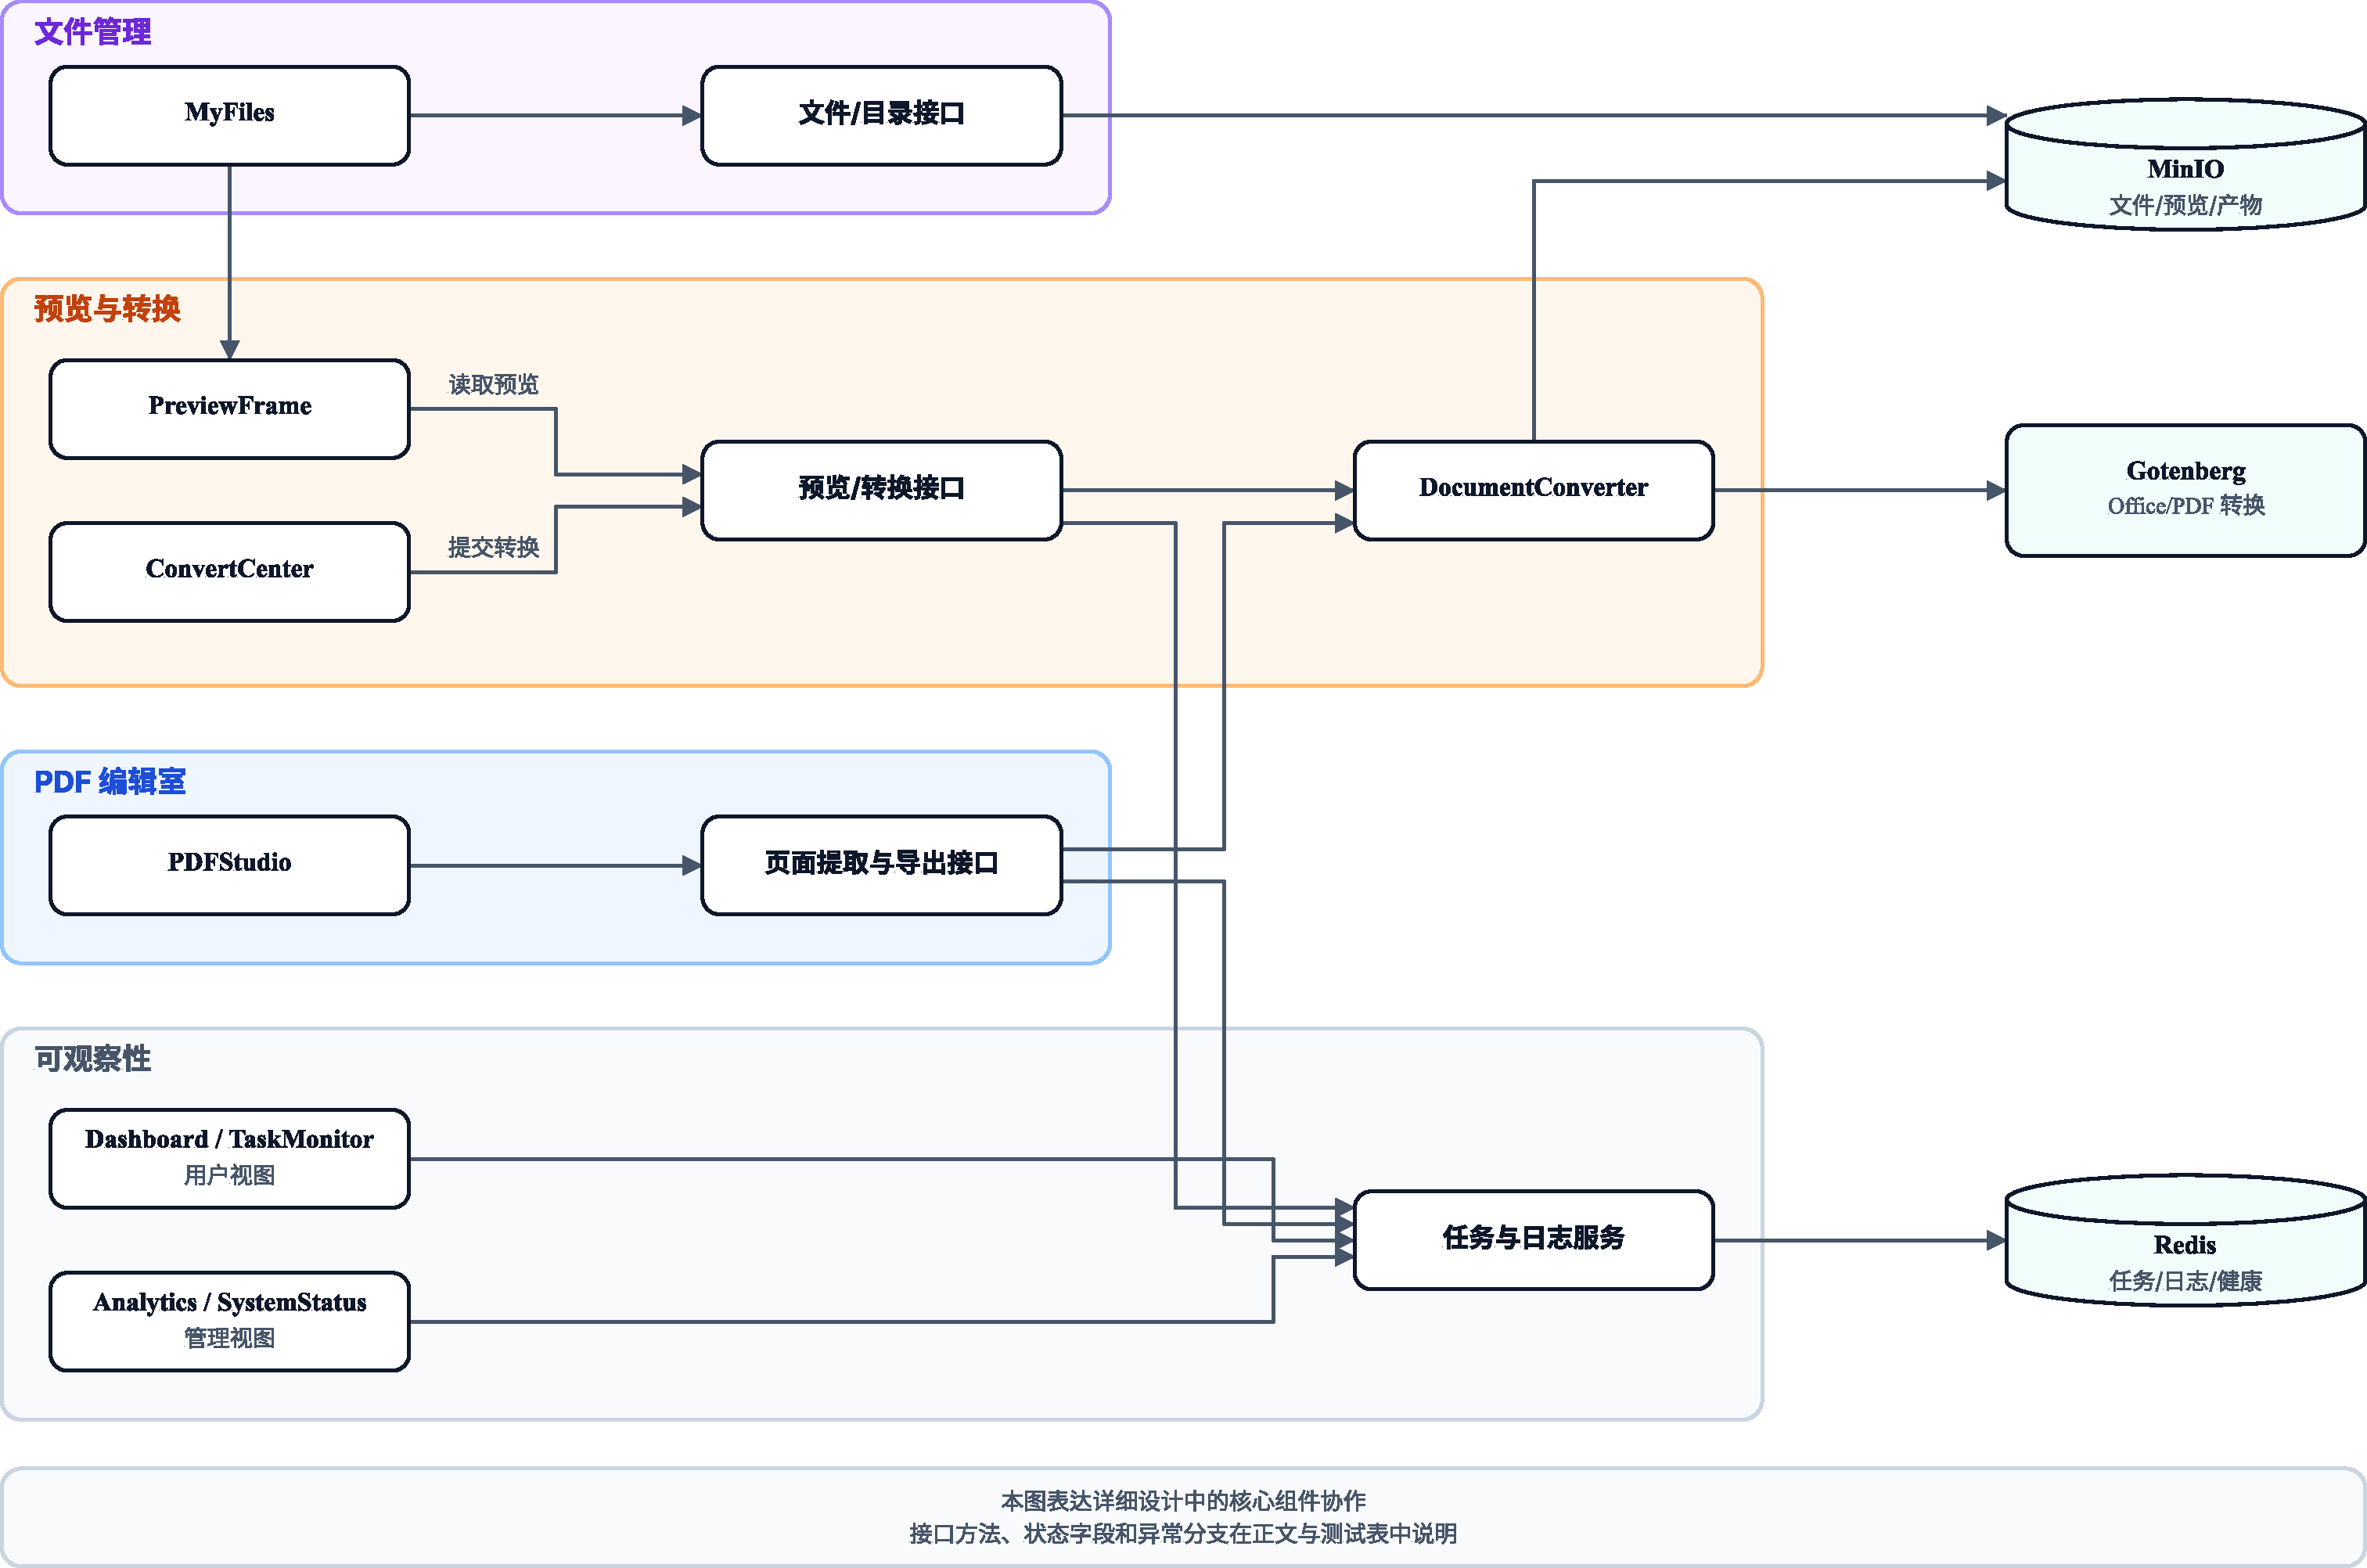
\includegraphics[width=0.96\textwidth,height=0.55\textheight,keepaspectratio]{figures-pdf/fig15-详细设计组件协作.pdf}
  \caption{核心功能详细设计组件协作图}
  \label{fig:chap05-component-design}
\end{figure}

\section{个人首页模块的实现}

\subsection{真实指标聚合}

个人首页由 \texttt{Dashboard.tsx} 实现，主要展示文件数量、存储空间、近期任务和失败提醒。该模块不使用静态计数，而是通过 \texttt{services/api.ts} 中的 \texttt{listFiles}、\texttt{listTasks}、\texttt{getTaskStats} 等函数读取后端数据。文件数量和容量来自 \texttt{/api/v1/files} 返回的 MinIO 对象元数据，任务成功和失败数量来自 Redis 任务索引。当前设计的关键点是让首页指标跟随真实文件处理行为变化，避免用户端完成转换后首页仍显示旧状态。

实现上，首页指标不直接读取浏览器缓存，而是把接口返回作为唯一可信来源。当前文件总量由递归文件列表聚合得到，任务数据由 \texttt{/api/v1/tasks/stats} 提供，近期失败可进一步通过 \texttt{/api/v1/tasks/recent-failures} 获取。这样处理的好处是页面刷新、前端重启或切换端侧后，指标仍能从后端状态恢复；缺点是首页依赖后端服务可用性，因此前端需要为接口异常提供明确提示，而不能默默显示零值。

\subsection{失败原因回溯}

失败任务提示依赖 \texttt{task\_queue.py} 和 \texttt{task\_tracker.py} 中的状态写入逻辑。当转换或 PDF 导出失败时，后端将错误原因写入任务对象的 \texttt{error} 字段，并通过任务接口返回给前端。前端在任务提示或历史列表中读取该字段，使用户能够区分格式不支持、文件损坏、转换服务不可用等不同故障来源。该实现使“失败计数”和“失败原因”具有同一后端来源。

从现场说明角度看，首页模块可以概括为“指标聚合层”：它本身不处理文件，也不执行转换，而是把文件管理、转换任务和异常状态聚合到一个用户可读入口。该设计降低了用户在多模块之间寻找结果的成本，也让后续管理端能够复用同一批任务与日志数据。

\section{我的文件模块的实现}

\subsection{上传、目录与类型分类}

我的文件模块由 \texttt{MyFiles.tsx} 实现，后端对应 \texttt{files.py} 与 \texttt{folders.py}。上传时，前端调用 \texttt{uploadFile(file,\{prefix,relativePath\})}，后端执行路径清洗、对象命名和 MinIO 写入，并通过 \texttt{log\_event} 记录文件上传事件。目录能力并不依赖传统关系数据库表，而是使用对象名前缀和 \texttt{.keep} 空对象表达。前端通过 \texttt{currentPrefix} 维护当前目录，文件类型由扩展名映射到 PDF、文档、表格、PPT、图片、文本、压缩包和其他类型。

该模块的关键实现边界在于：前端只负责组织交互状态和展示分类，不直接操作对象存储；对象命名、路径合法性和文件内容写入均在后端完成。后端 \texttt{\_sanitize\_path} 会拒绝包含危险路径片段的输入，避免用户通过相对路径影响系统目录。文件上传完成后，前端重新拉取列表而不是本地拼接文件项，保证显示内容与 MinIO 中的实际对象保持一致。

上传后的容量展示采用对象大小聚合结果，与第 3 章式 \ref{eq:req-storage-size} 保持一致。前端只展示接口返回的文件大小和汇总容量，不把本地选择文件时的临时大小作为最终值。这样即使后端对文件名、路径或对象前缀进行了清洗，页面上看到的仍然是对象存储确认后的结果。

\subsection{目录操作与对象移动}

文件移动由 \texttt{moveToFolder} 调用 \texttt{/api/v1/folders/move} 完成。后端路由 \texttt{folders.py} 校验目标目录是否存在，并通过 MinIO 的复制和删除完成对象迁移。对文件夹删除、重命名和移动等操作，系统需要处理前缀递归关系，避免将父目录移动到自身子目录中造成路径循环。表 \ref{tab:chap05-code-map} 汇总了用户端主要模块与后端实现位置。

由于对象存储没有真正的目录表，所有目录操作最终都会落到对象名前缀变化上。系统把“路径前缀”作为目录语义，把“对象名”作为文件唯一定位依据，使文件夹浏览、文件移动和文件下载可以共享同一套对象模型。这种设计简化了数据层，但要求后端在移动和删除时格外注意级联对象范围，避免误删预览缓存或转换产物。

\begin{table}[H]
  \centering
  \small
  \caption{核心模块代码位置与数据链路}
  \label{tab:chap05-code-map}
  \begin{tabularx}{\textwidth}{llXX}
    \toprule
    模块 & 前端位置 & 后端位置 & 主要数据对象 \\
    \midrule
    我的文件 & \texttt{MyFiles} & 文件/目录路由 & MinIO 文件对象、目录前缀 \\
    文件预览 & \texttt{PreviewFrame} & 预览路由与预览服务 & 预览类型、预览缓存 \\
    转换中心 & \texttt{ConvertCenter} & 转换路由与转换服务 & Redis 任务、转换产物 \\
    PDF 编辑室 & \texttt{PDFStudio} & PDF 处理接口与转换服务 & 页面配置、批注对象、PDF 产物 \\
    管理驾驶舱 & \texttt{Analytics} & 任务、日志、健康与分析接口 & 实时指标、历史分析样本 \\
    \bottomrule
  \end{tabularx}
\end{table}

图 \ref{fig:chap05-file-manual-group} 展示了文件管理模块的运行结果。左图为根目录与文件夹视图，右图为上传后的文件列表和类型筛选视图。可以看到，文件对象进入列表后保留名称、大小、更新时间和格式标识，说明前端列表与 MinIO 对象元数据已经建立映射。

\begin{figure}[H]
  \centering
  \begin{subfigure}{0.48\textwidth}
    \centering
    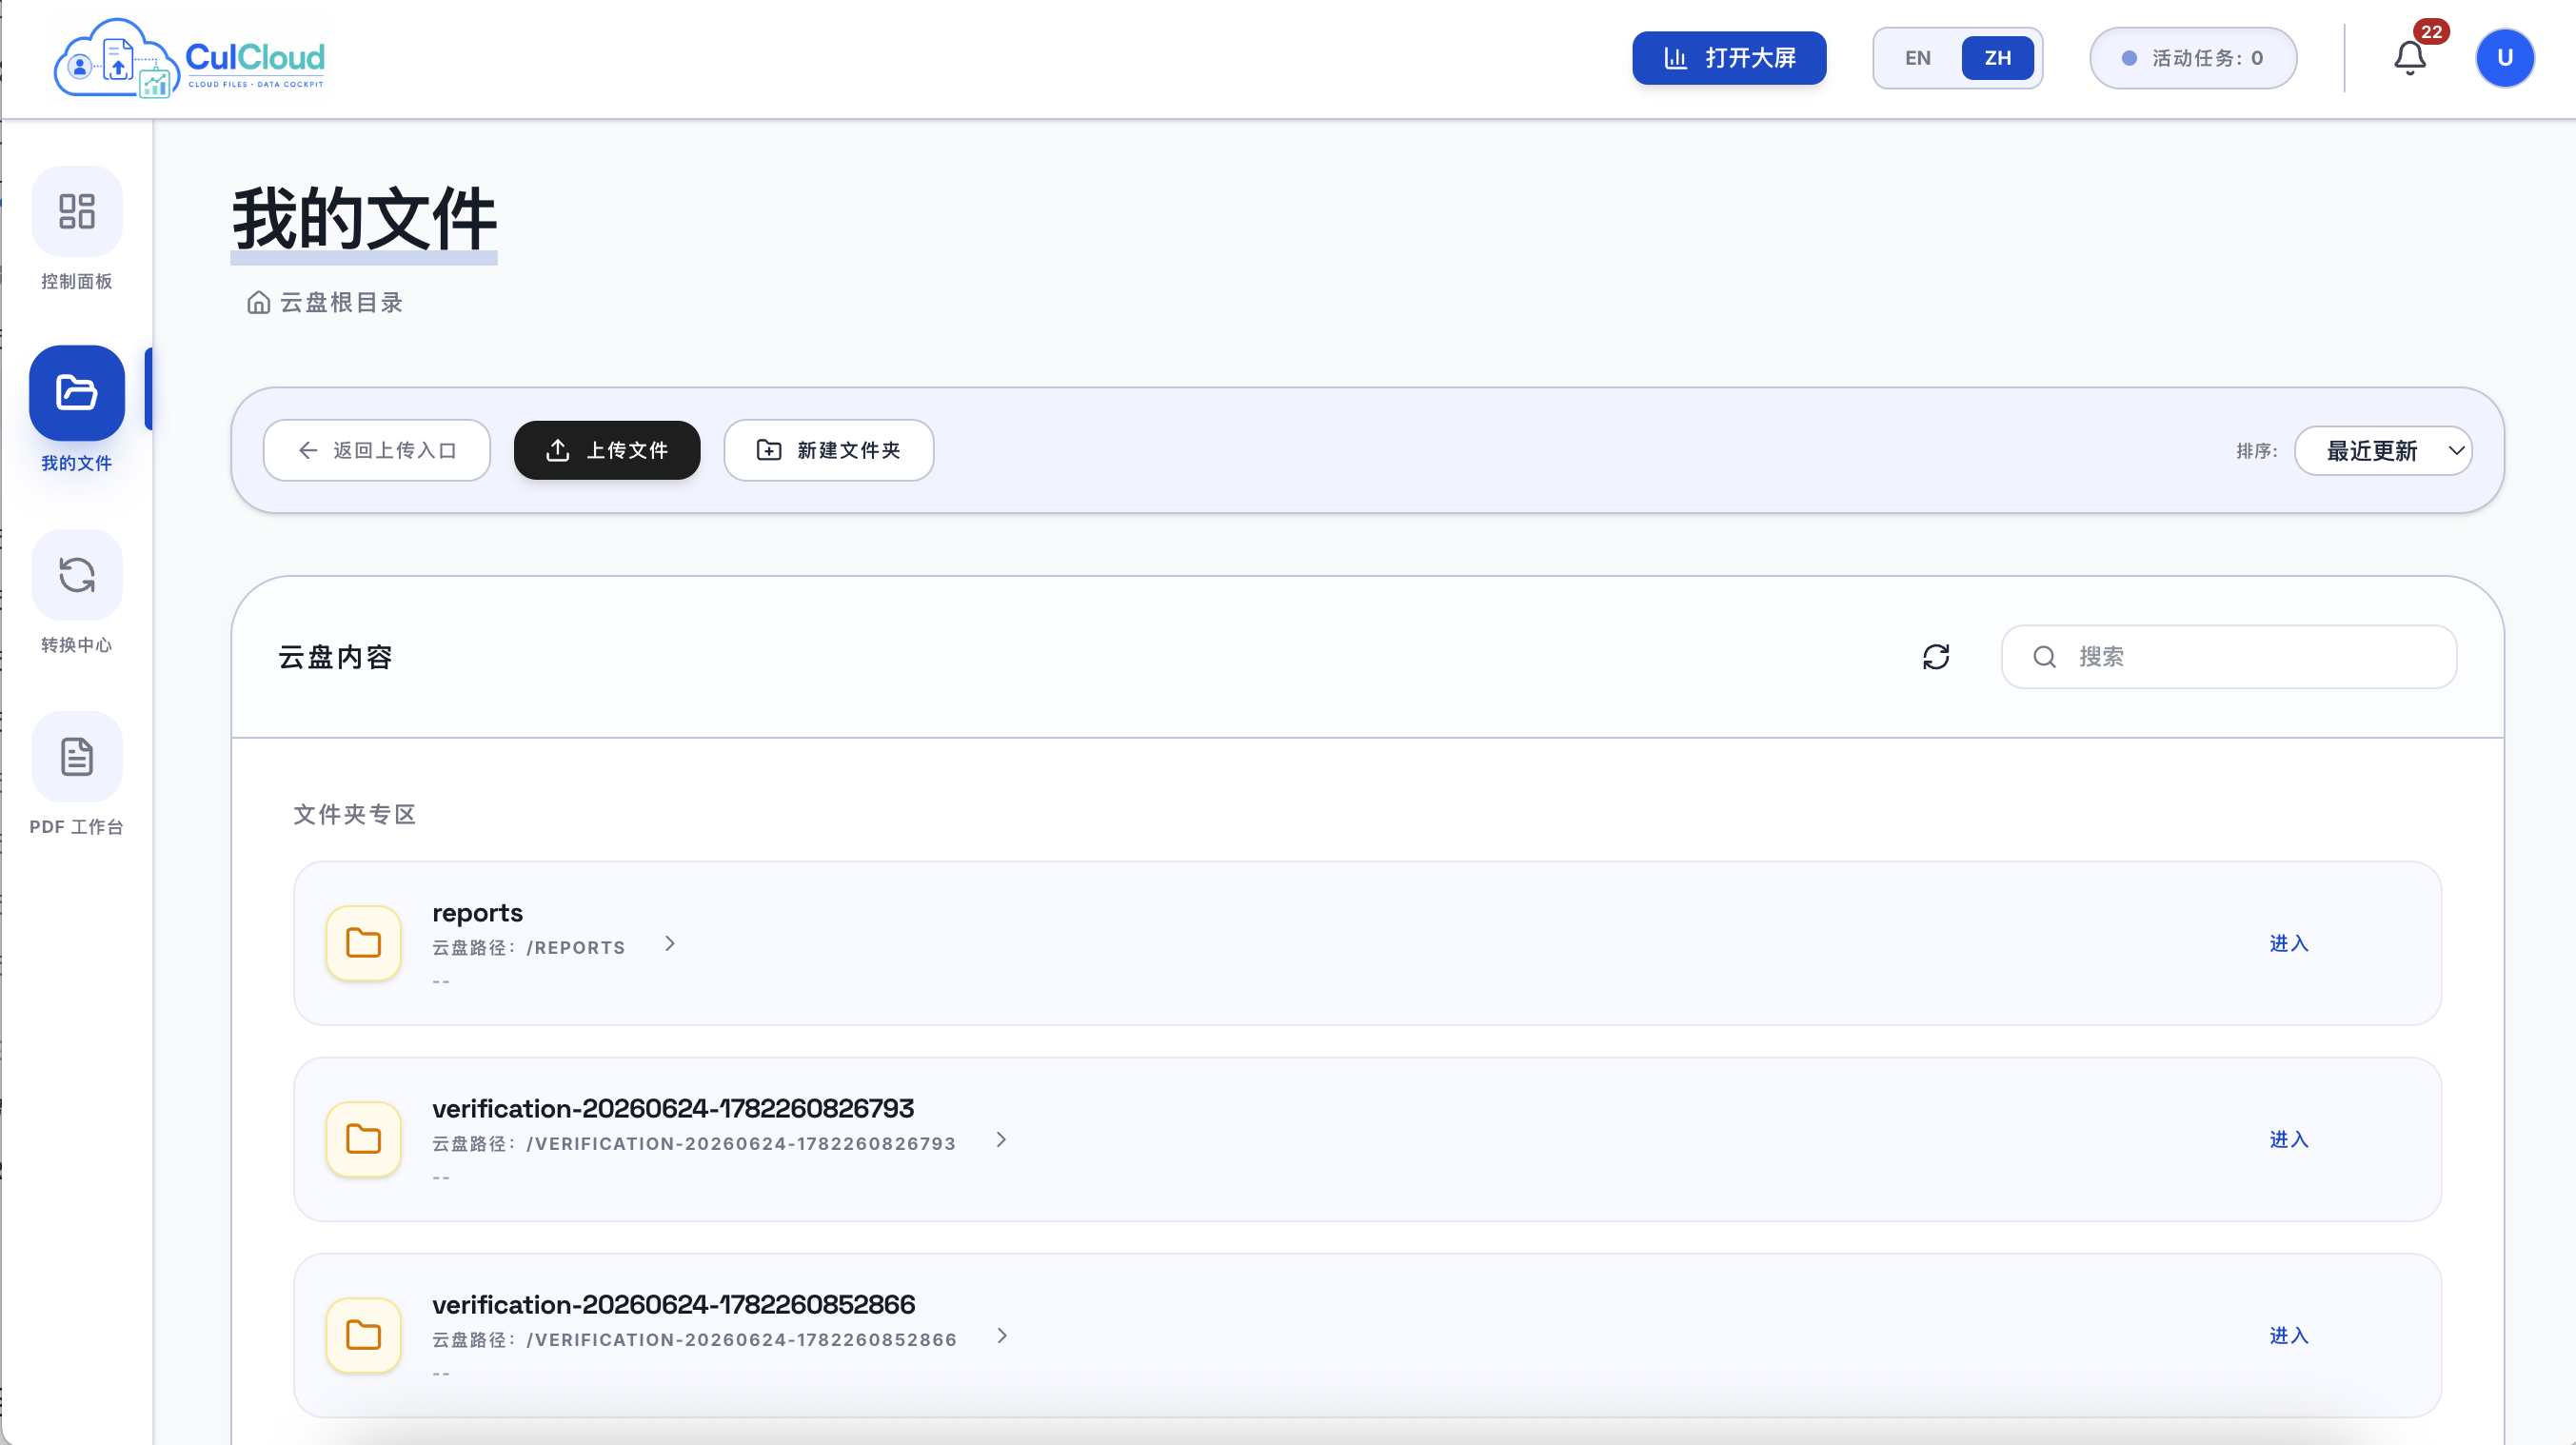
\includegraphics[width=\linewidth,height=0.25\textheight,keepaspectratio]{figures-png/ui/manual/fig05-manual-01-file-folders-root.png}
    \caption{目录与文件夹视图}
  \end{subfigure}
  \hfill
  \begin{subfigure}{0.48\textwidth}
    \centering
    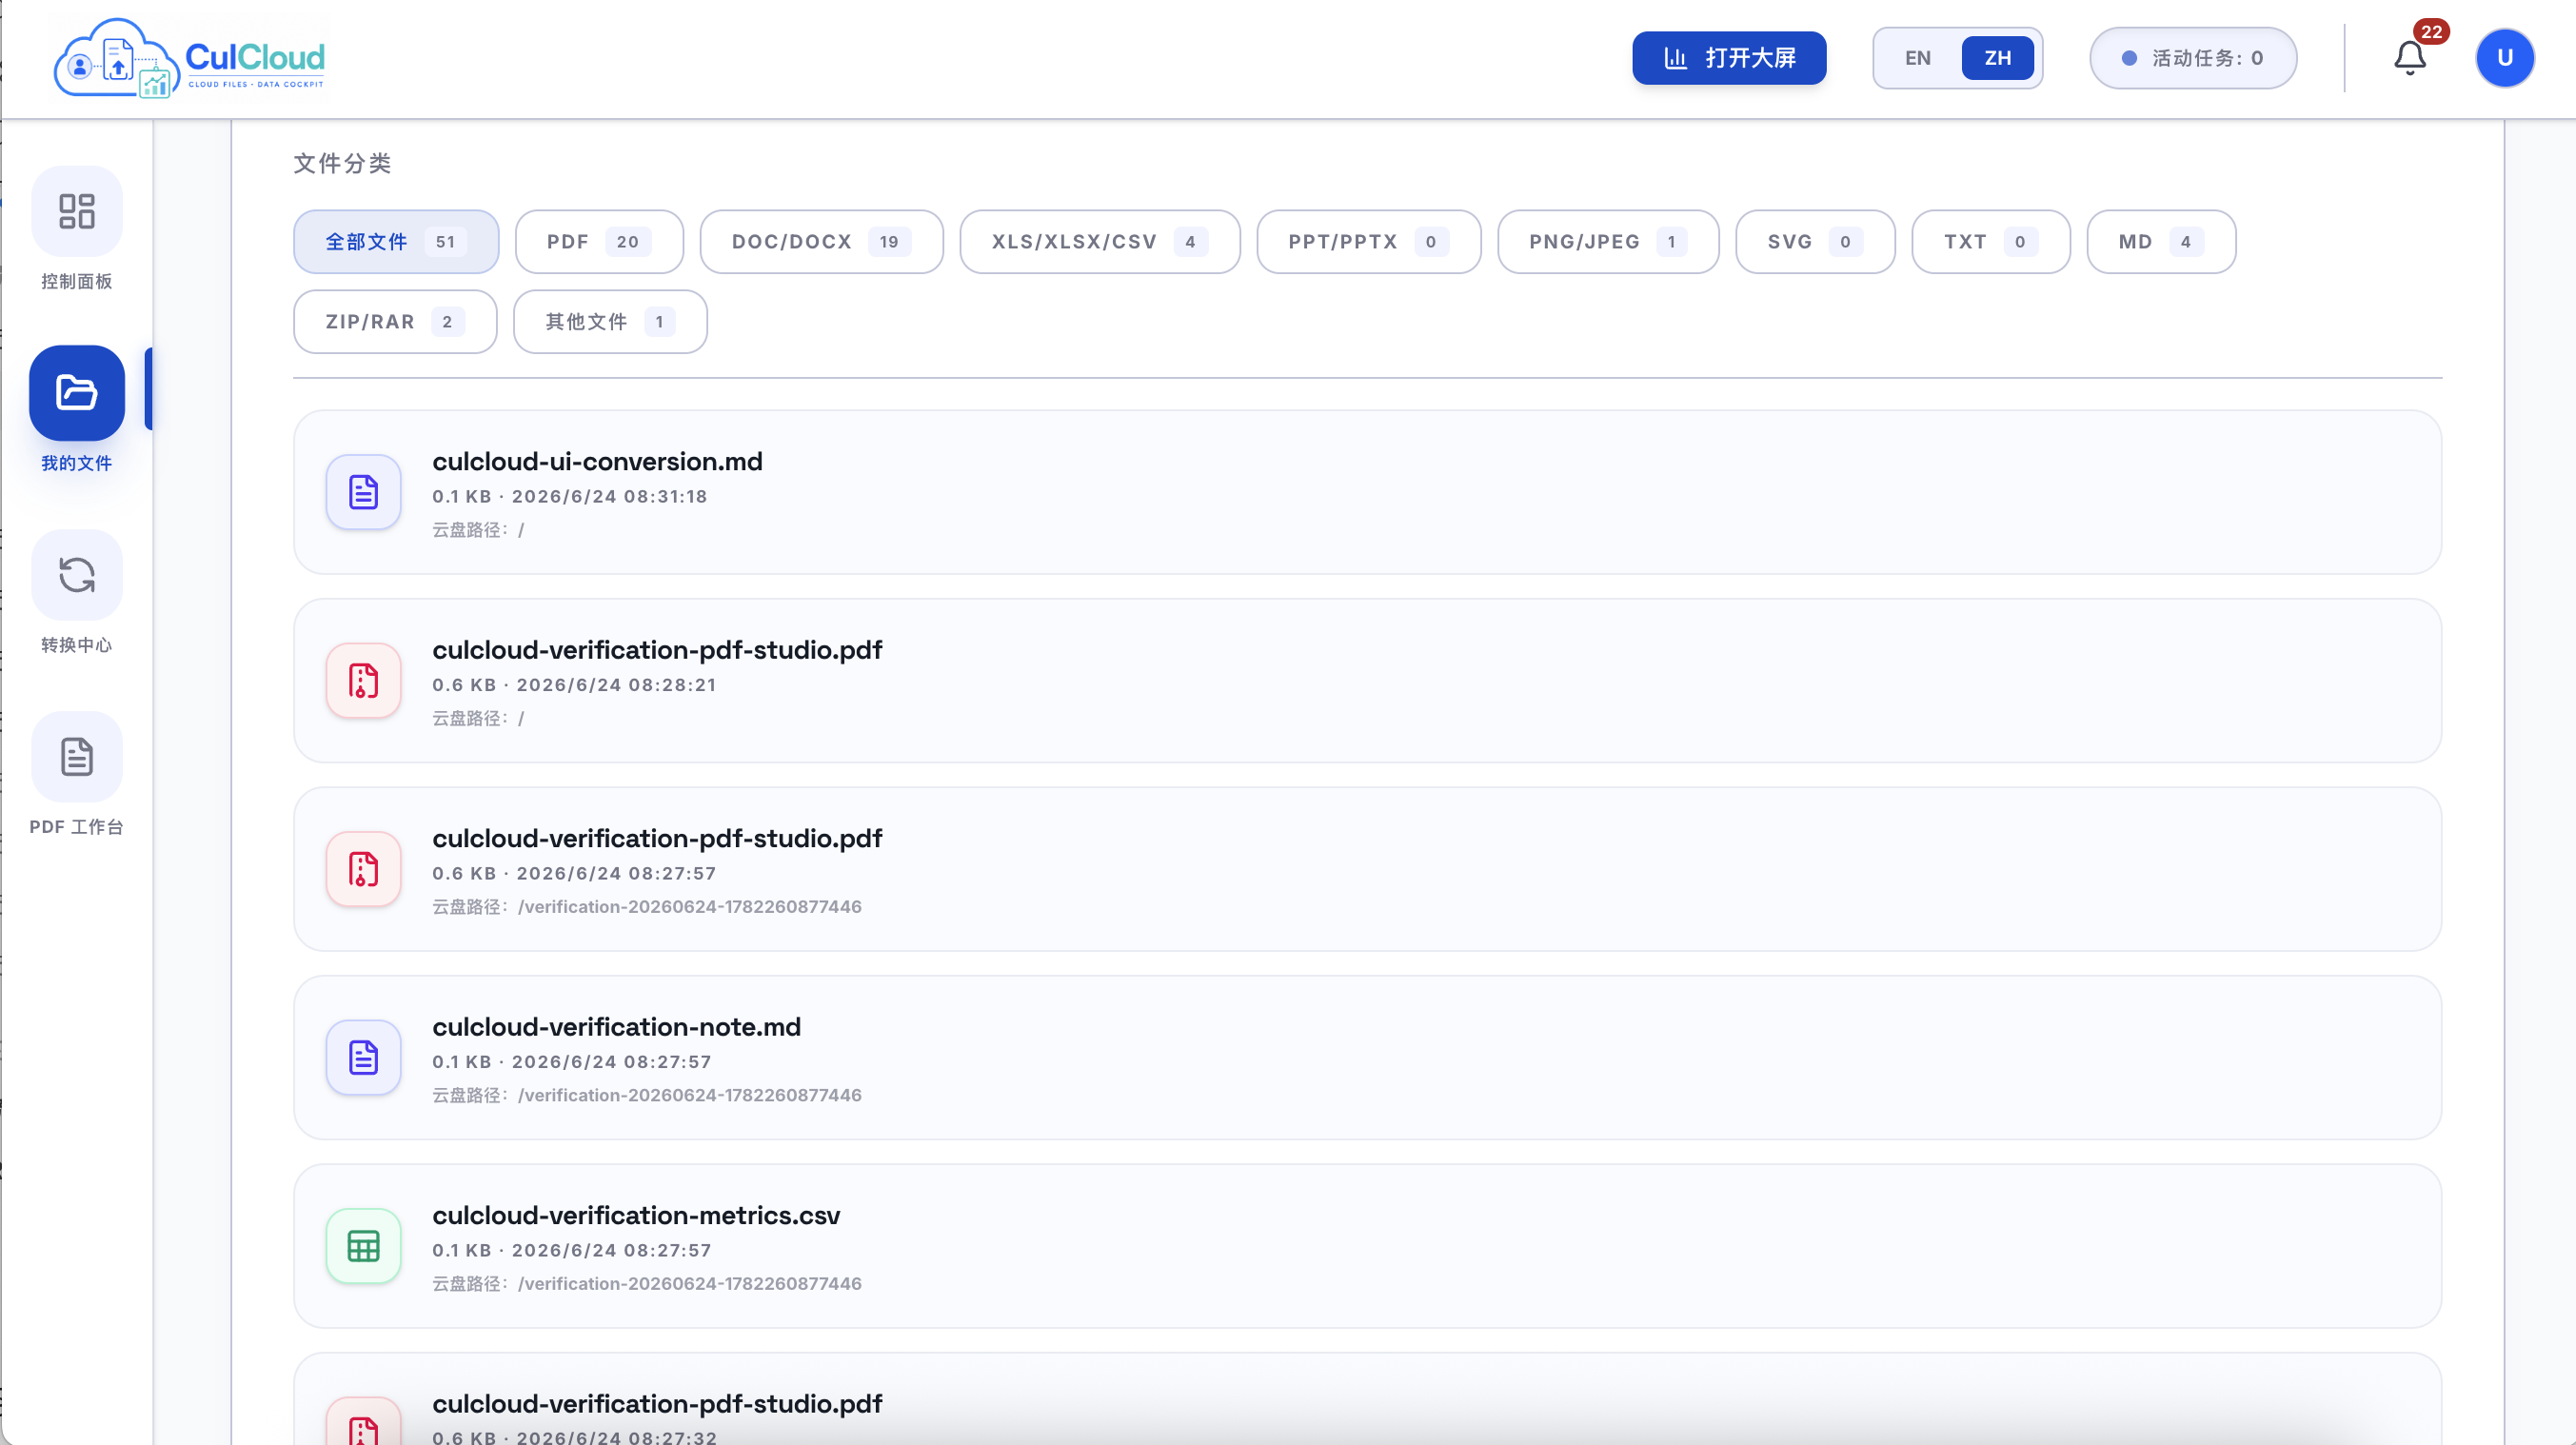
\includegraphics[width=\linewidth,height=0.25\textheight,keepaspectratio]{figures-png/ui/manual/fig05-manual-02-file-uploaded-list.png}
    \caption{上传后文件列表}
  \end{subfigure}
  \caption{文件管理模块界面结果图}
  \label{fig:chap05-file-manual-group}
\end{figure}

\section{文件预览模块的实现}

\subsection{预览类型识别}

文件预览由前端 \texttt{PreviewFrame} 和后端 \texttt{preview.py}、\texttt{services/preview.py} 协同实现。后端 \texttt{get\_preview\_metadata} 根据扩展名判断 \texttt{preview\_type}，并返回 \texttt{content\_url}。PDF、图片、音频和视频可直接通过内容接口返回；TXT 使用文本响应；Markdown 和 CSV 转换为隔离 HTML；Office 文件通过 Gotenberg 或转换服务生成 PDF 缓存。该设计使预览模块不要求前端理解所有文件解析细节，前端只需根据 \texttt{preview\_type} 选择对应展示组件。

预览接口分为元数据接口与内容接口两层。元数据接口负责说明文件是否可预览、预览类型和内容地址；内容接口负责返回字节流或渲染后的 HTML。这样做可以让前端先决定展示容器，再按需加载实际内容，避免大文件在列表阶段被提前读取。对于 Office 文件，缓存对象名由源文件信息计算得到，重复预览时优先复用缓存，减少转换服务压力。

第 4 章算法 \ref{alg:preview-dispatch} 已给出预览分派规则。本章关注其实现位置：扩展名识别、内容地址生成和不可预览状态由后端完成，前端只根据返回的 \texttt{preview\_type} 选择 PDF、图片、音视频、文本或 HTML 容器。

预览分派还承担异常兜底职责。若文件类型无法识别，接口应明确返回不可预览状态，而不是让前端反复尝试打开内容地址；若 Office 预览缓存生成失败，页面应保留下载入口和错误提示，避免用户误以为文件丢失；若 Markdown 或 CSV 内容较长，前端只负责展示后端生成的隔离内容，不把整份文本写入全局状态。这样可以把解析风险限制在预览模块内部。

缓存策略也影响用户体验。对于同一对象的重复预览，系统优先复用已生成的 PDF 或 HTML 缓存；当源文件发生移动或重命名时，内容接口仍应以对象名为准重新定位文件。该设计让预览模块既能减少转换服务压力，又能保持与文件管理模块的一致性。

\subsection{结构化内容渲染}

Markdown 和 CSV 的预览是该模块的关键实现。Markdown 需要在后端转换为 HTML，同时避免用户上传内容直接污染主页面；CSV 需要读取字节流、处理编码并生成表格化视图。图 \ref{fig:chap05-preview-manual-group} 展示了 PDF、Markdown 和 CSV 三类预览结果，三者分别对应二进制文档、标记文本和结构化表格。

从实现风险看，CSV 与 Markdown 预览比图片和 PDF 更容易出现编码、HTML 安全和长内容排版问题。因此后端采用独立响应内容承载渲染结果，前端通过预览框加载，既保留可读性，也减少对主页面状态树的影响。该策略适合课程资料中常见的配置文件、实验数据表和说明文档。

\begin{figure}[H]
  \centering
  \begin{subfigure}{0.32\textwidth}
    \centering
    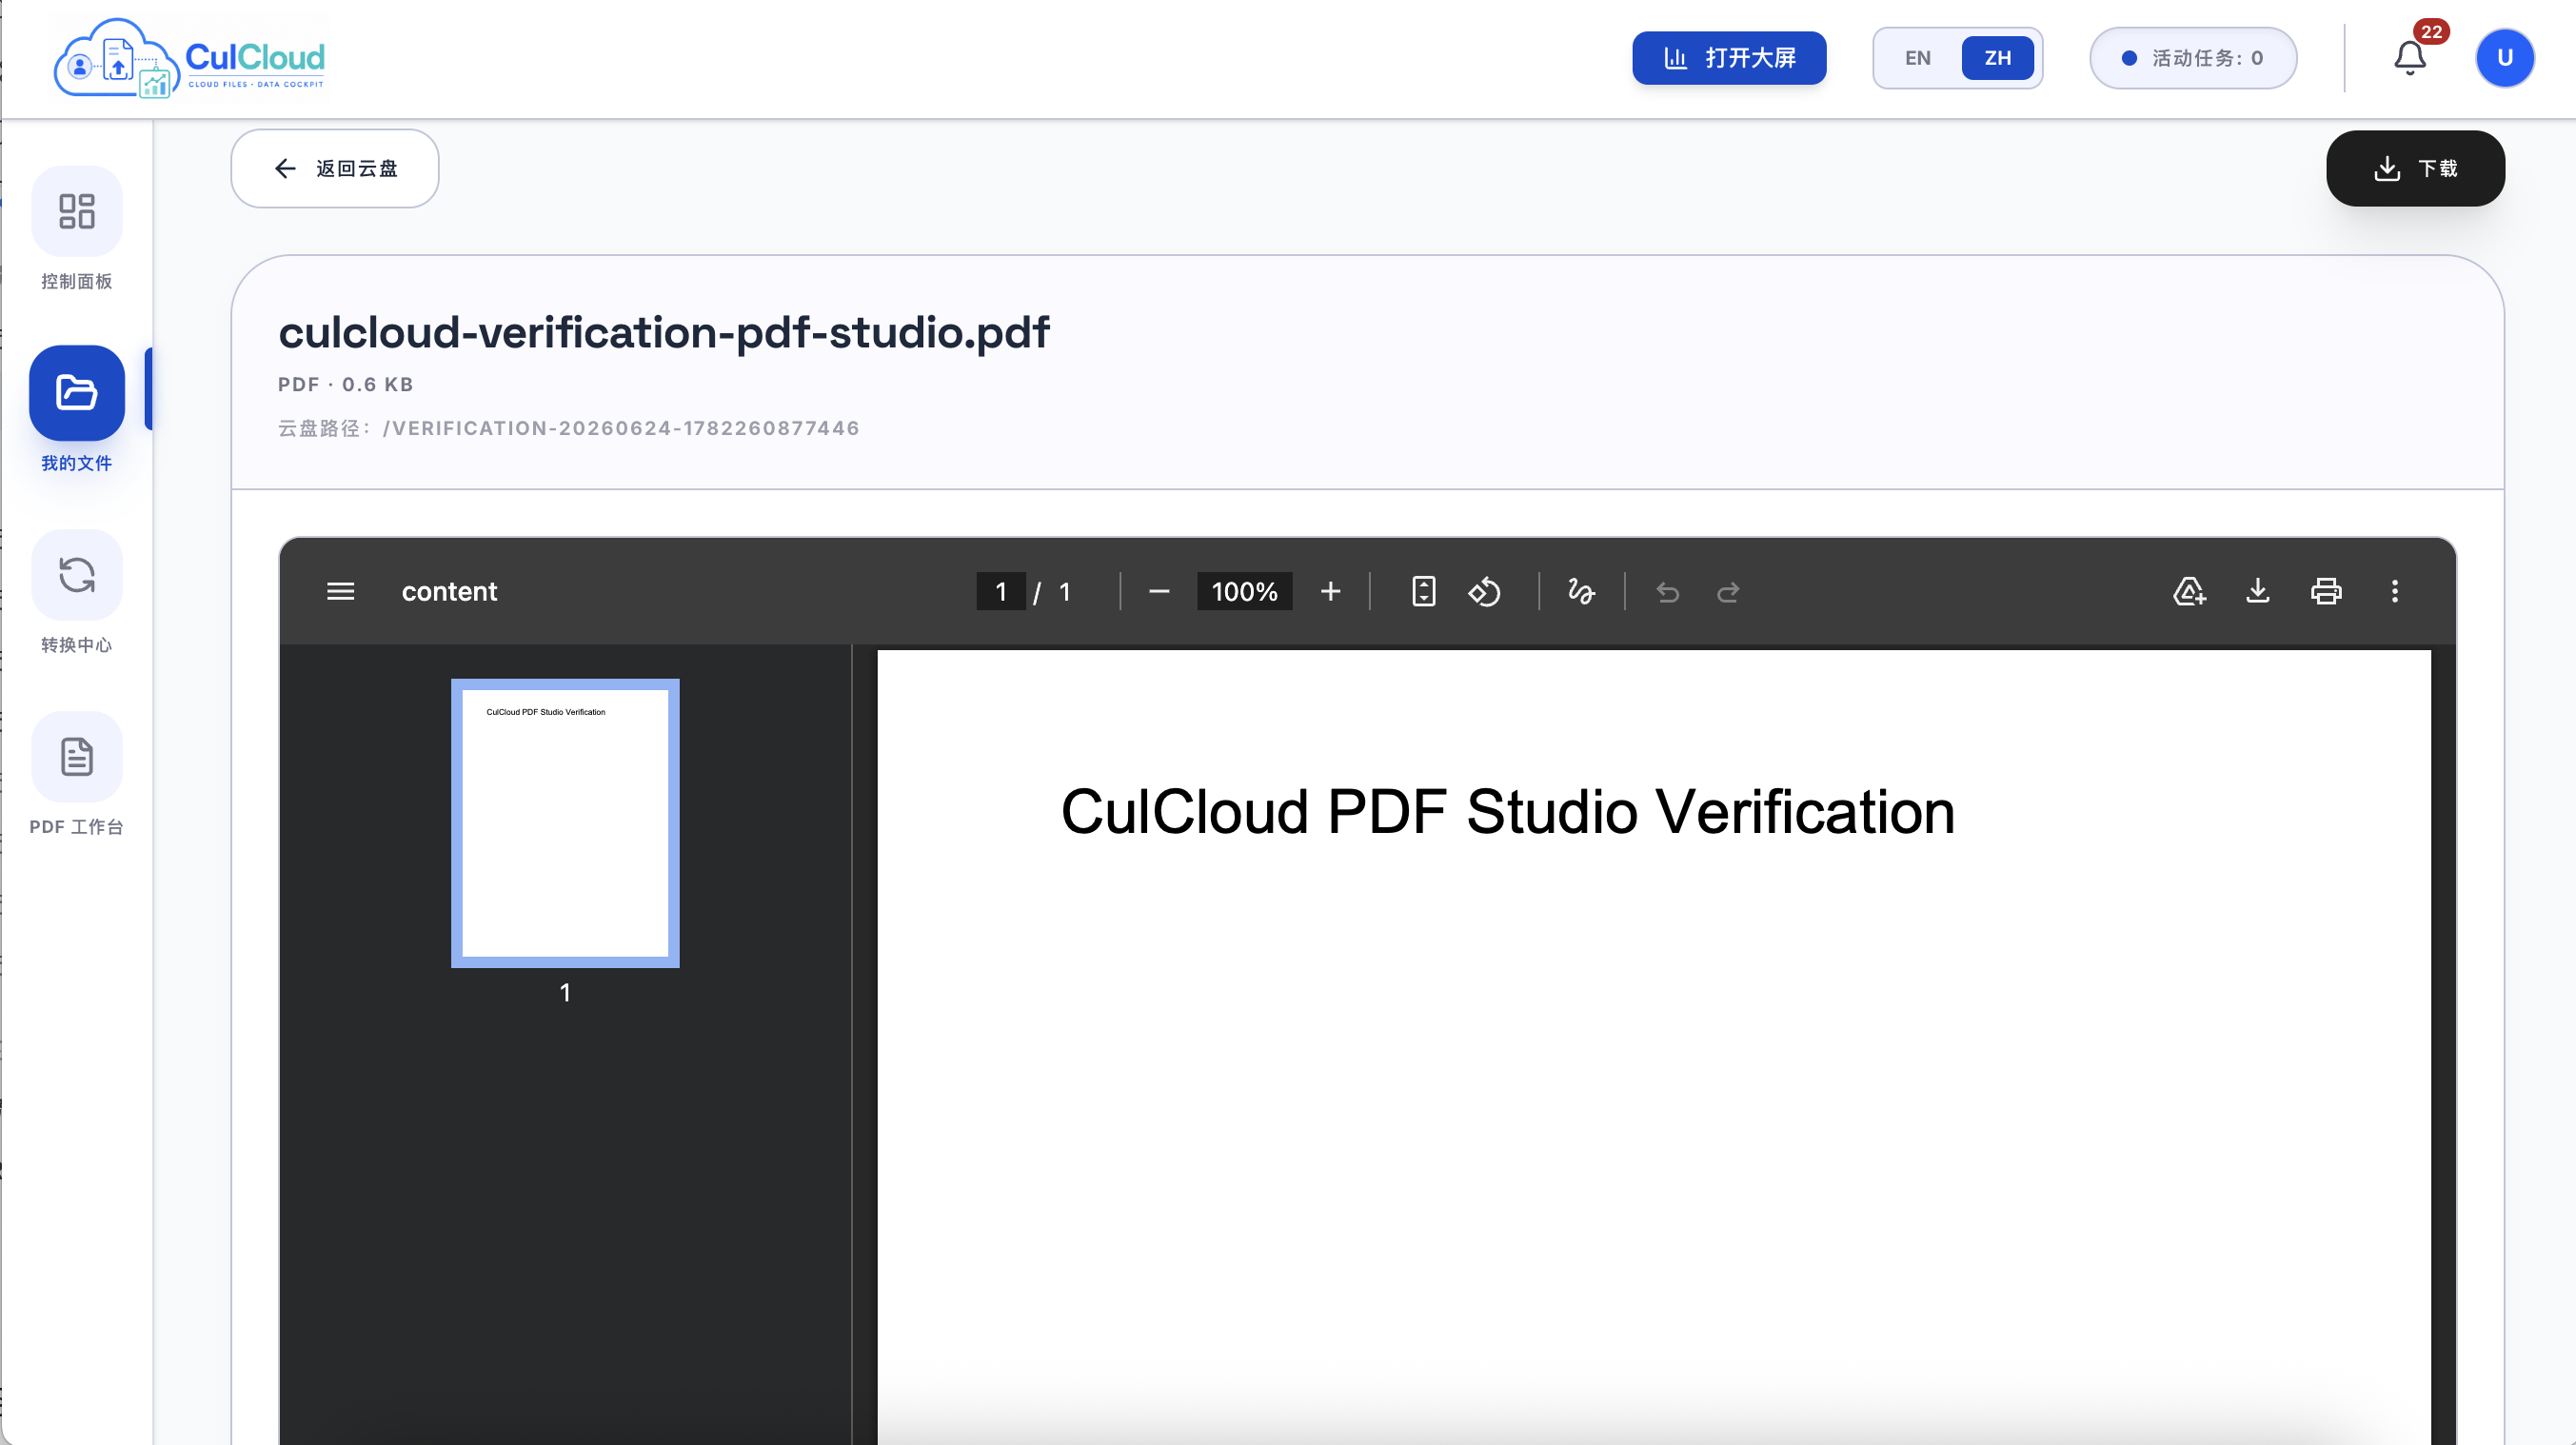
\includegraphics[width=\linewidth,height=0.20\textheight,keepaspectratio]{figures-png/ui/manual/fig05-manual-03-pdf-preview-result.png}
    \caption{PDF 预览}
  \end{subfigure}
  \hfill
  \begin{subfigure}{0.32\textwidth}
    \centering
    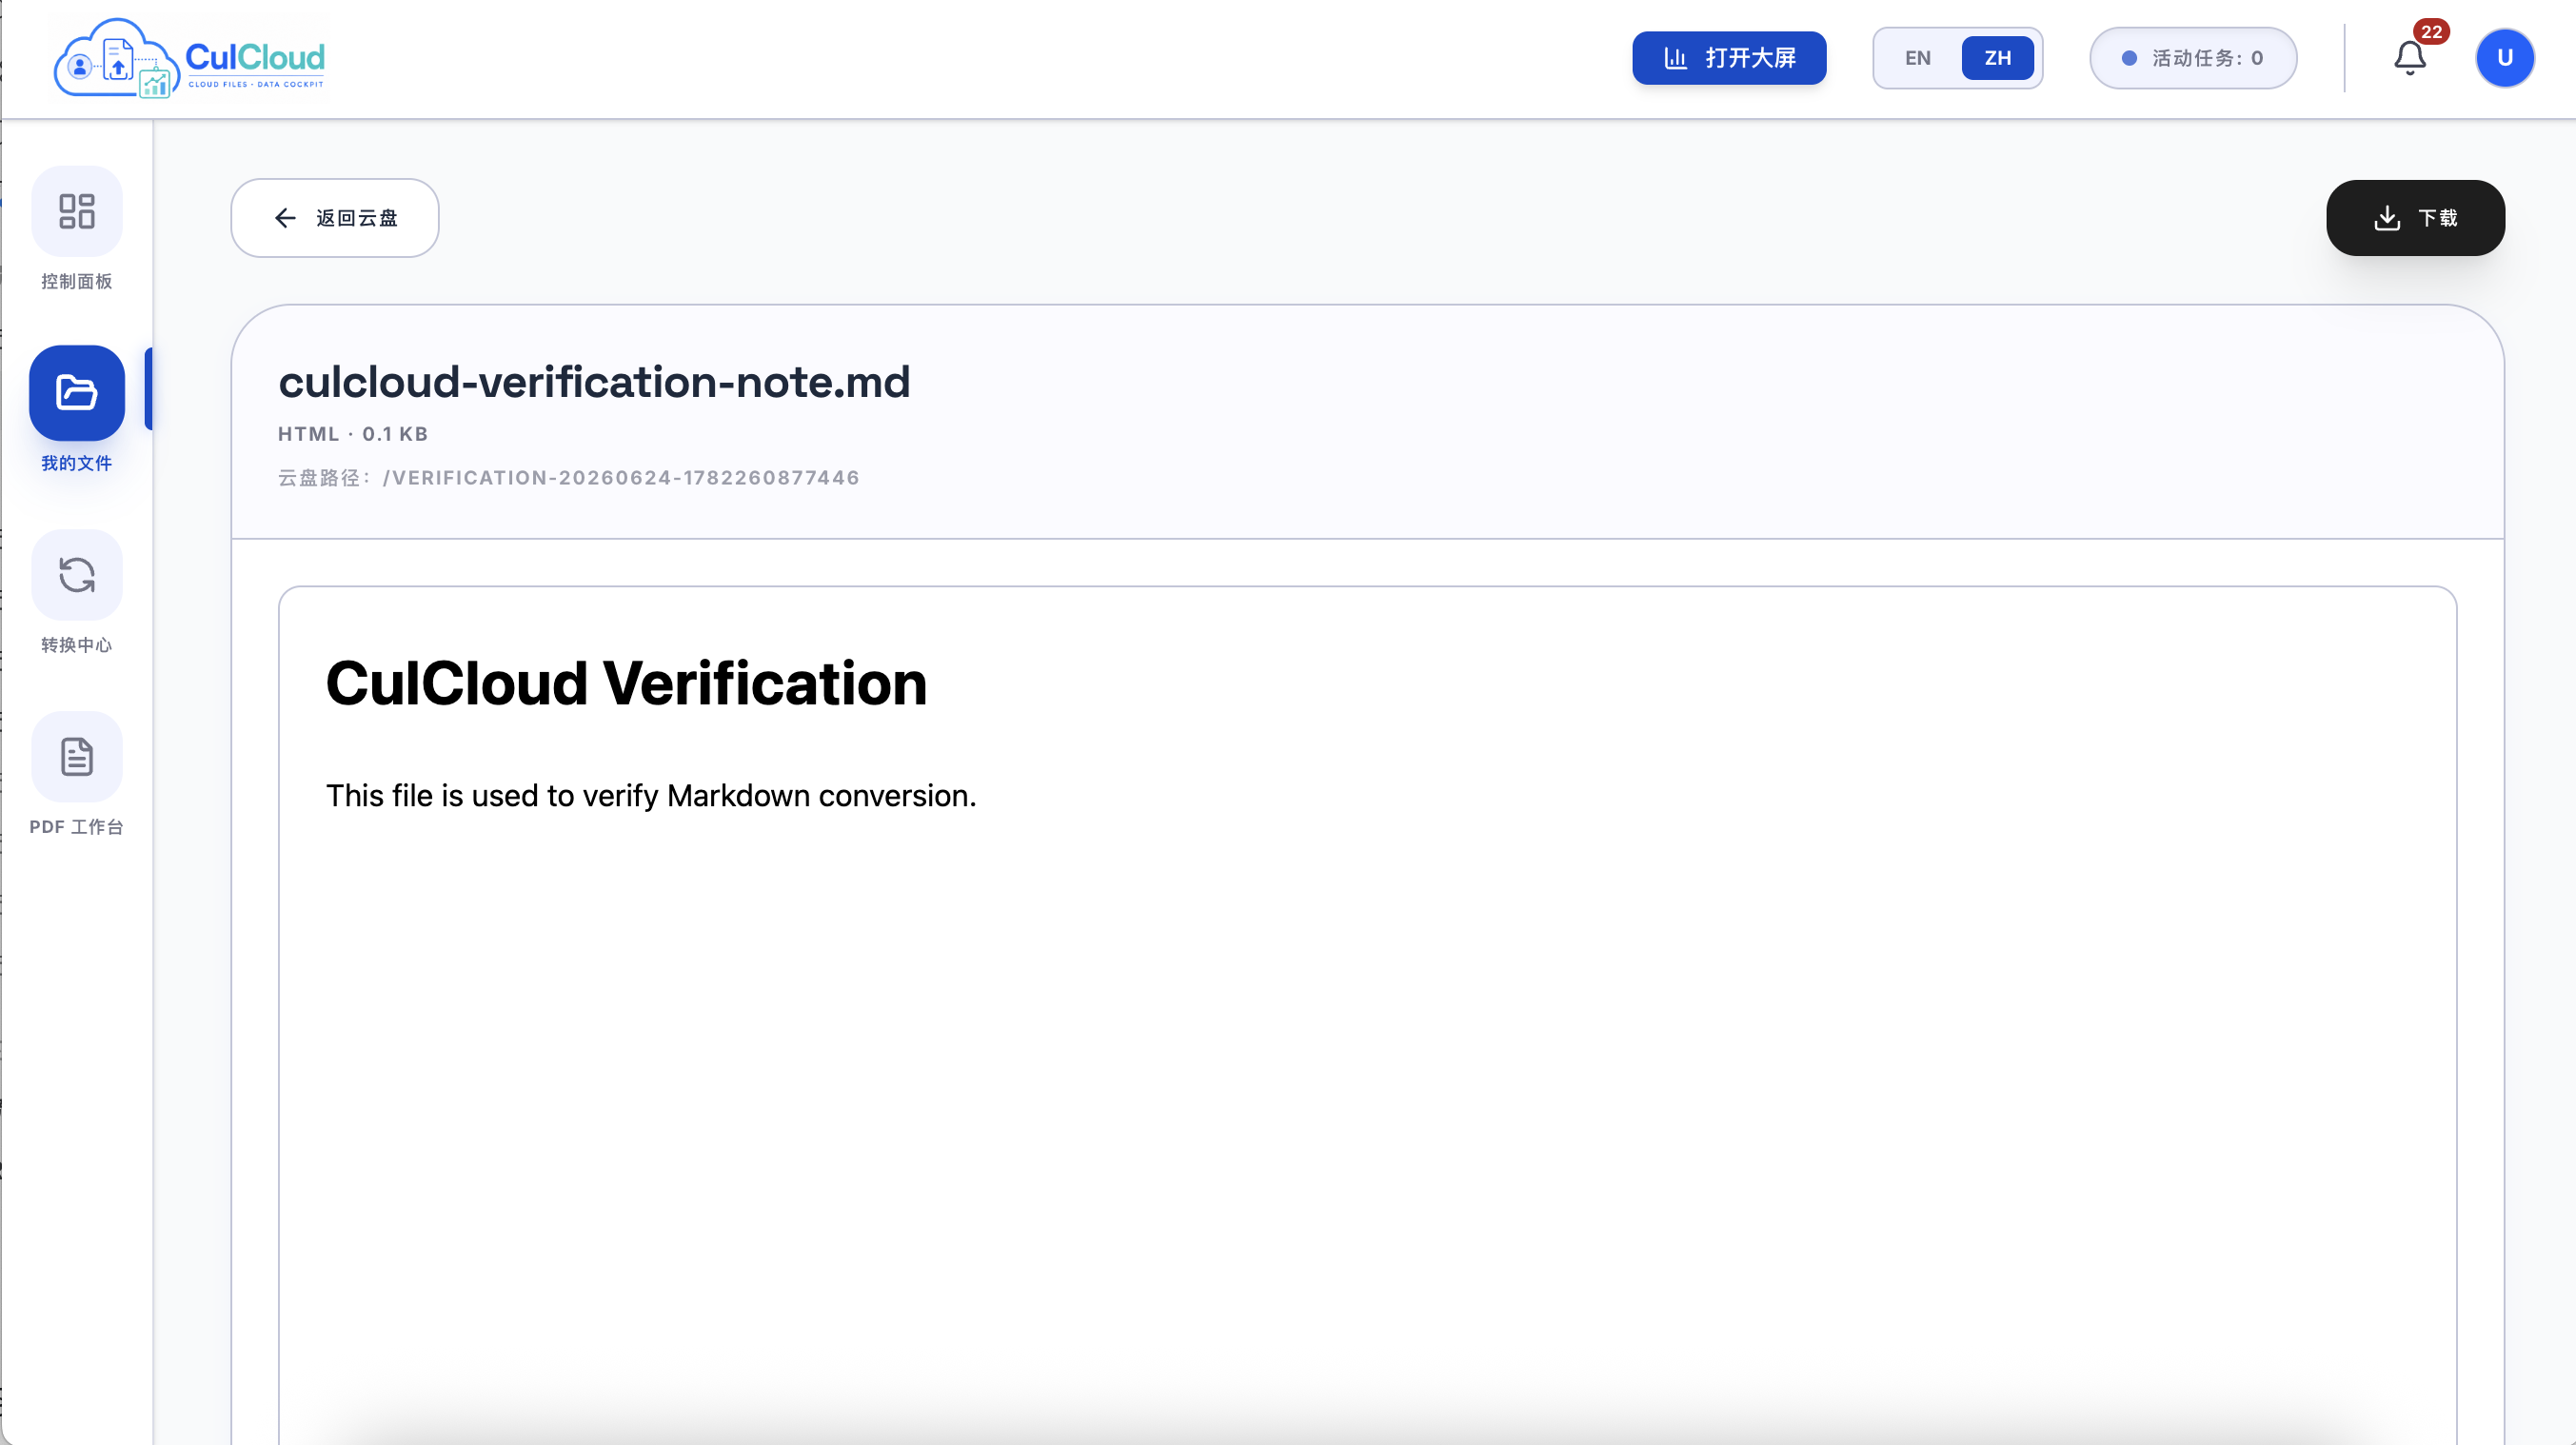
\includegraphics[width=\linewidth,height=0.20\textheight,keepaspectratio]{figures-png/ui/manual/fig05-manual-04-markdown-preview-result.png}
    \caption{Markdown 预览}
  \end{subfigure}
  \hfill
  \begin{subfigure}{0.32\textwidth}
    \centering
    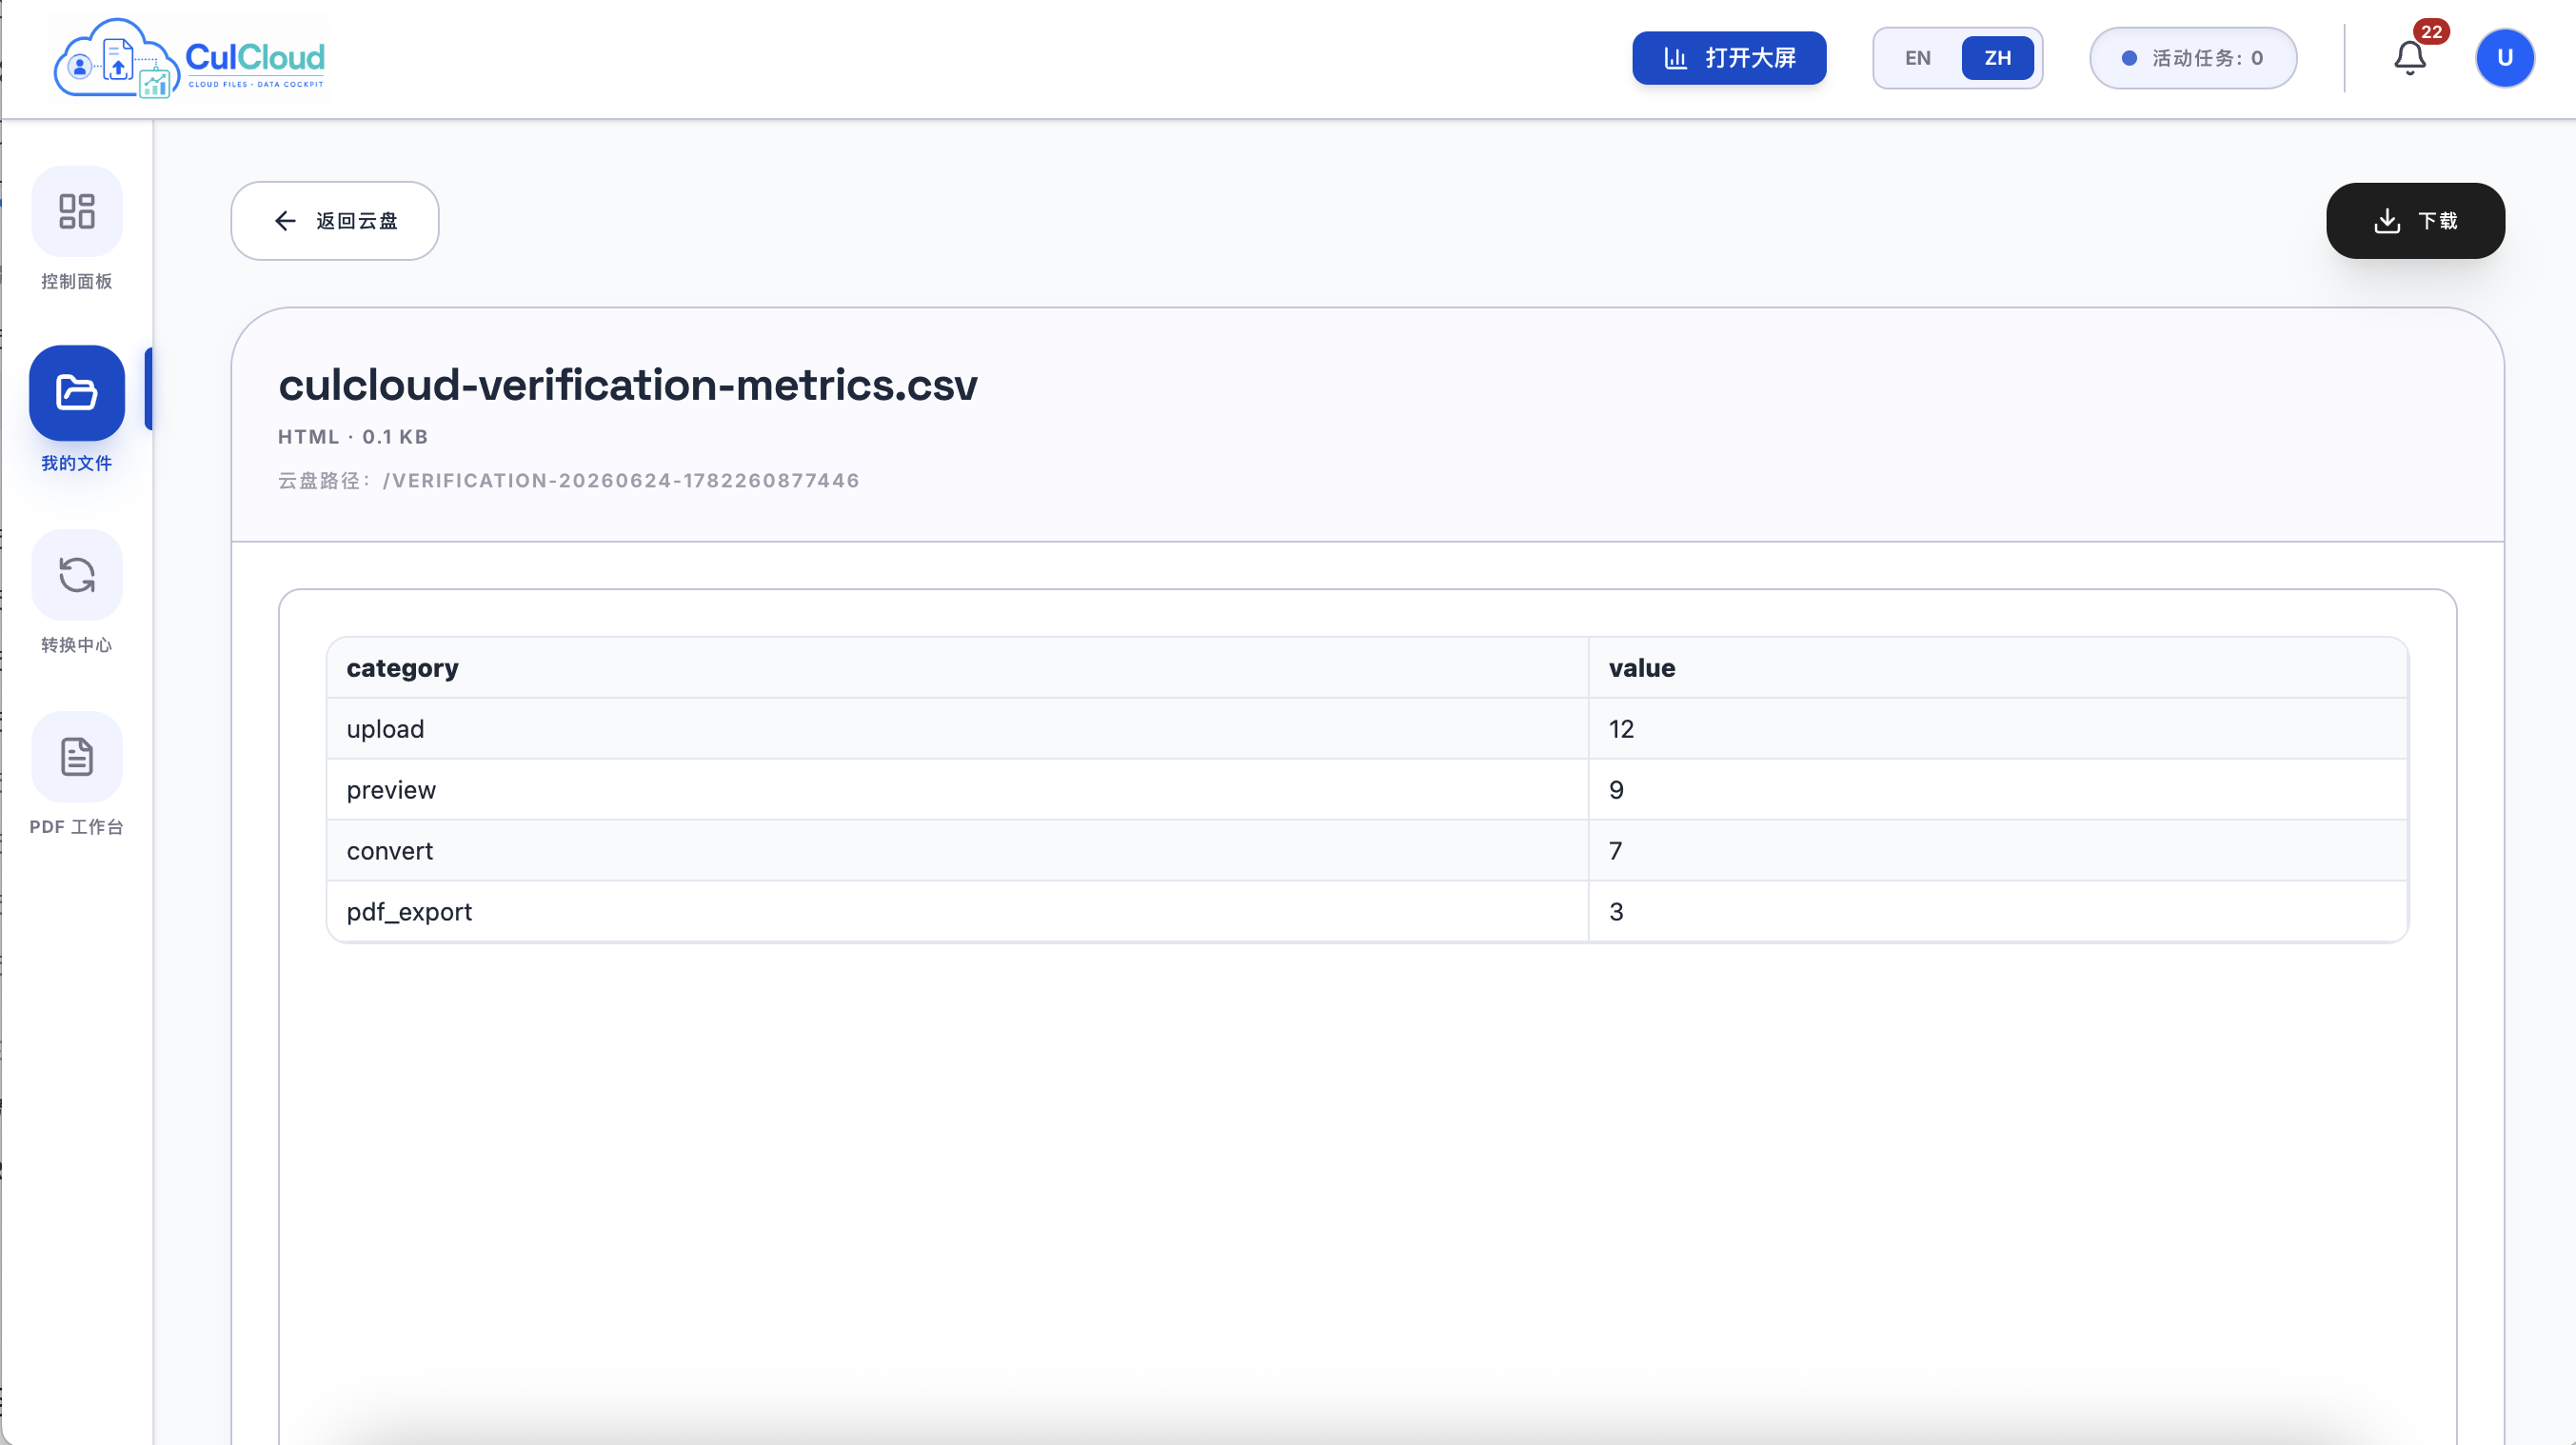
\includegraphics[width=\linewidth,height=0.20\textheight,keepaspectratio]{figures-png/ui/manual/fig05-manual-05-csv-preview-result.png}
    \caption{CSV 预览}
  \end{subfigure}
  \caption{文件预览模块界面结果图}
  \label{fig:chap05-preview-manual-group}
\end{figure}

\section{转换中心模块的实现}

\subsection{白名单与能力矩阵}

转换中心由 \texttt{ConvertCenter.tsx} 实现，后端对应 \texttt{routers/convert.py} 和 \texttt{services/converter.py}。系统在前后端都维护 P0 白名单：前端 \texttt{P0\_WHITELIST} 控制用户可选择的转换项，后端 \texttt{\_assert\_p0\_whitelist} 在 API 层再次拒绝未开放格式。这样即使前端被绕过，后端也不会执行未验证的转换路径。转换能力信息由 \texttt{/api/v1/convert/capabilities} 返回，便于前端按文件扩展名过滤目标格式。

白名单设计体现了系统的能力边界。项目并没有把所有库中理论可调用的转换函数都暴露给用户，而是只开放经过页面、接口和产物验证的高频链路。前端负责降低误操作概率，后端负责最终安全约束。该双层约束可以在后续扩展格式时逐项放开，而不会影响已经稳定的转换路径。

\subsection{异步任务执行}

转换任务提交后，后端调用 \texttt{set\_task\_status(task\_id, pending)} 写入初始状态，并通过 FastAPI BackgroundTasks 调用 \texttt{async\_convert\_task}。后台任务读取源文件，执行 \texttt{DocumentConverter} 中对应方法，例如 \texttt{word\_to\_pdf}、\texttt{csv\_to\_pdf}、\texttt{markdown\_to\_pdf}、\texttt{svg\_to\_png} 等。成功后，结果写入 MinIO 的 \texttt{conversions/} 前缀，任务状态更新为 \texttt{success} 并返回 API 代理下载地址；失败时写入 \texttt{failed} 与错误原因。图 \ref{fig:chap05-conversion-success} 展示了转换完成后的当前任务状态。

第 4 章算法 \ref{alg:async-task-process} 概括了转换与 PDF 导出共用的异步处理模式。代码实现中，转换中心对应 \texttt{async\_convert\_task}，PDF 编辑室对应 \texttt{async\_pdf\_process\_task}，二者都通过任务状态写入函数保持等待、处理中、成功和失败的一致语义。这样前端轮询、任务监控和管理驾驶舱读取到的是同一套状态来源。

前端轮询并不是无限循环，而是以第 4 章式 \ref{eq:polling-stop} 作为终止条件。\texttt{ConvertCenter.tsx} 和 \texttt{PDFStudio.tsx} 在读取到成功或失败终态后停止定时查询，避免任务已经结束后仍持续请求后端。

转换结果下载采用 API 代理地址，而不是直接暴露 MinIO 内部地址。这样可以避免浏览器跳转到对象存储端口后出现 Office 压缩包内部 XML 被直接打开等异常体验，也让下载行为继续受后端接口控制。任务状态轮询由前端定时触发，轮询终止条件是任务进入成功或失败终态，避免长期无意义请求。

\begin{figure}[H]
  \centering
  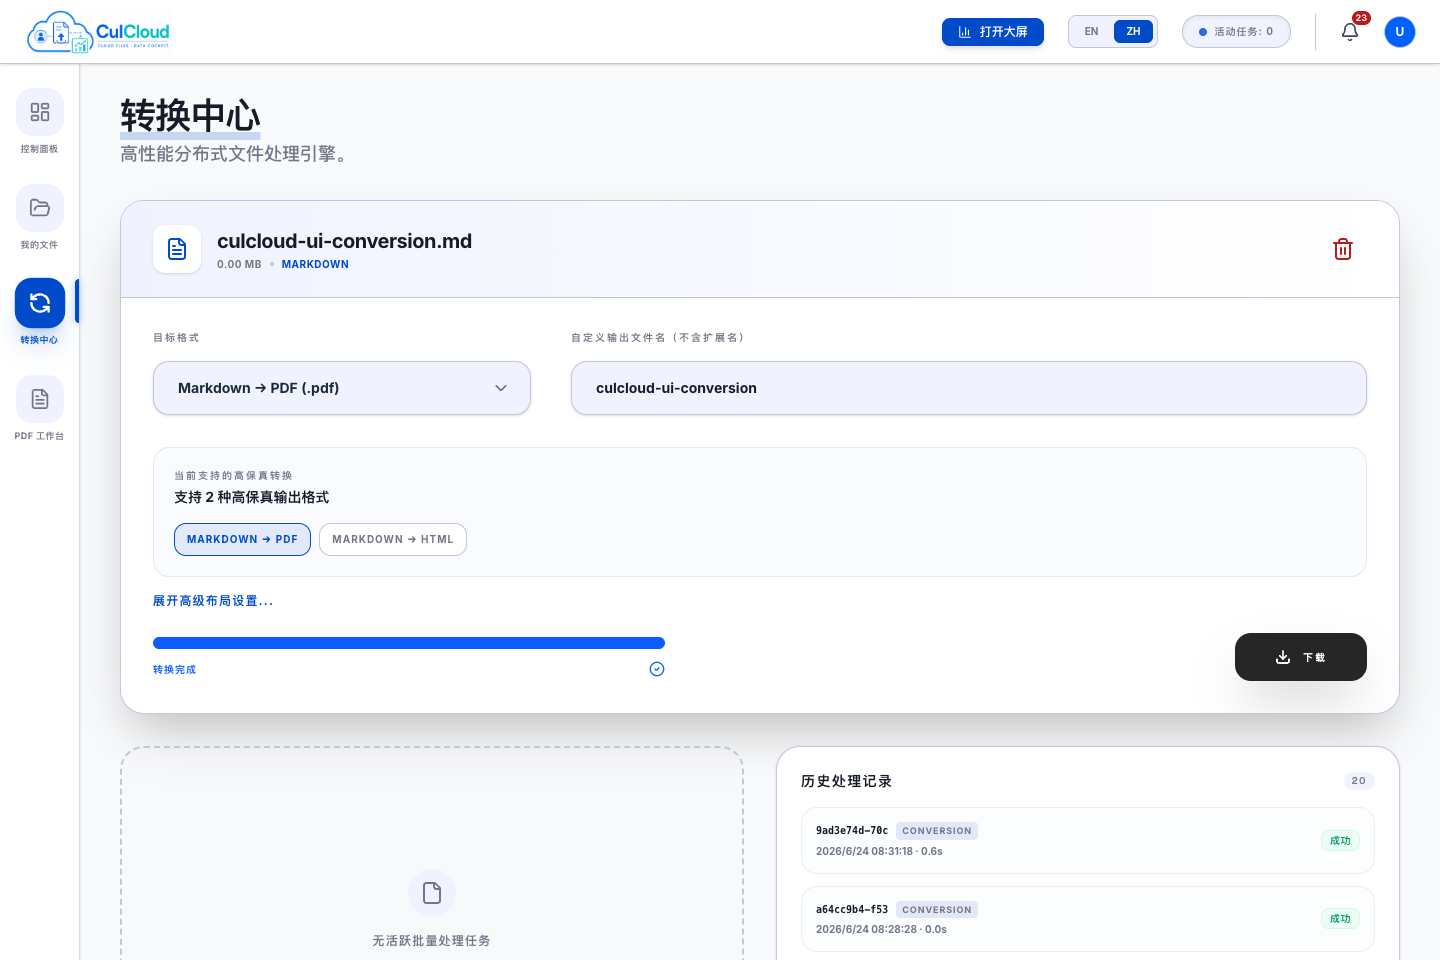
\includegraphics[width=0.92\textwidth,height=0.45\textheight,keepaspectratio]{figures-png/ui/fig05-10-conversion-current-success.png}
  \caption{转换中心任务完成界面结果图}
  \label{fig:chap05-conversion-success}
\end{figure}

\section{PDF 编辑室模块的实现}

\subsection{页面工作区}

PDF 编辑室由 \texttt{PDFStudio.tsx} 实现，核心状态包括 \texttt{WorkspacePage}、\texttt{Annotation}、当前工具、缩放比例和选中对象。用户选择 PDF 后，前端调用 \texttt{extractPdfPages}，后端使用 \texttt{DocumentConverter.pdf\_to\_images} 将每页转换为 PNG，并保存到 \texttt{previews/\{preview\_id\}/page\_N.png}。前端据此构建页面工作区，支持页面选择、排序、旋转、删除和批注。

PDF 工作区的设计采用“页面数组 + 批注数组”的状态模型。页面数组保存源对象、页码、旋转角度和尺寸信息，批注数组保存工具类型、坐标点、文本和颜色。排序与删除操作只改变页面数组，不直接修改源 PDF；导出时再由后端根据最终配置生成新文件。该方式使编辑过程可撤回、可重组，也避免频繁写入大体积 PDF 文件。

\subsection{批注与导出}

批注对象记录工具类型、坐标点、文本、颜色和线宽。导出时，前端将页面配置和批注数组提交给 \texttt{processPdf}，后端 \texttt{async\_pdf\_process\_task} 调用 \texttt{DocumentConverter.process\_pdf\_pages} 重组 PDF 并写入批注。图 \ref{fig:chap05-pdf-manual-group} 展示了 PDF 编辑工作区和导出后文件结果。该组图说明页面操作不是停留在浏览器状态，而是能够生成可打开的新 PDF 文件。

批注导出的难点在于坐标映射。前端操作发生在缩放后的画布上，后端写入发生在 PDF 页面坐标系中，因此导出配置必须携带前端画布宽高，并在后端按比例换算。对于文本批注，还需要加载适合中英文混排的字体，保证导出文件中的中文文本不会出现字符间距异常。

第 4 章式 \ref{eq:pdf-coordinate-map} 和算法 \ref{alg:pdf-export} 已给出坐标映射与导出规则。实现层面，前端提交页面配置数组和批注数组，后端在 \texttt{process\_pdf\_pages} 中读取源页面、应用旋转和顺序、换算批注坐标、加载 CJK 字体并写入新 PDF。这样 PDF 编辑室的交互状态能够转化为可打开的文件产物。

\begin{figure}[H]
  \centering
  \begin{subfigure}{0.48\textwidth}
    \centering
    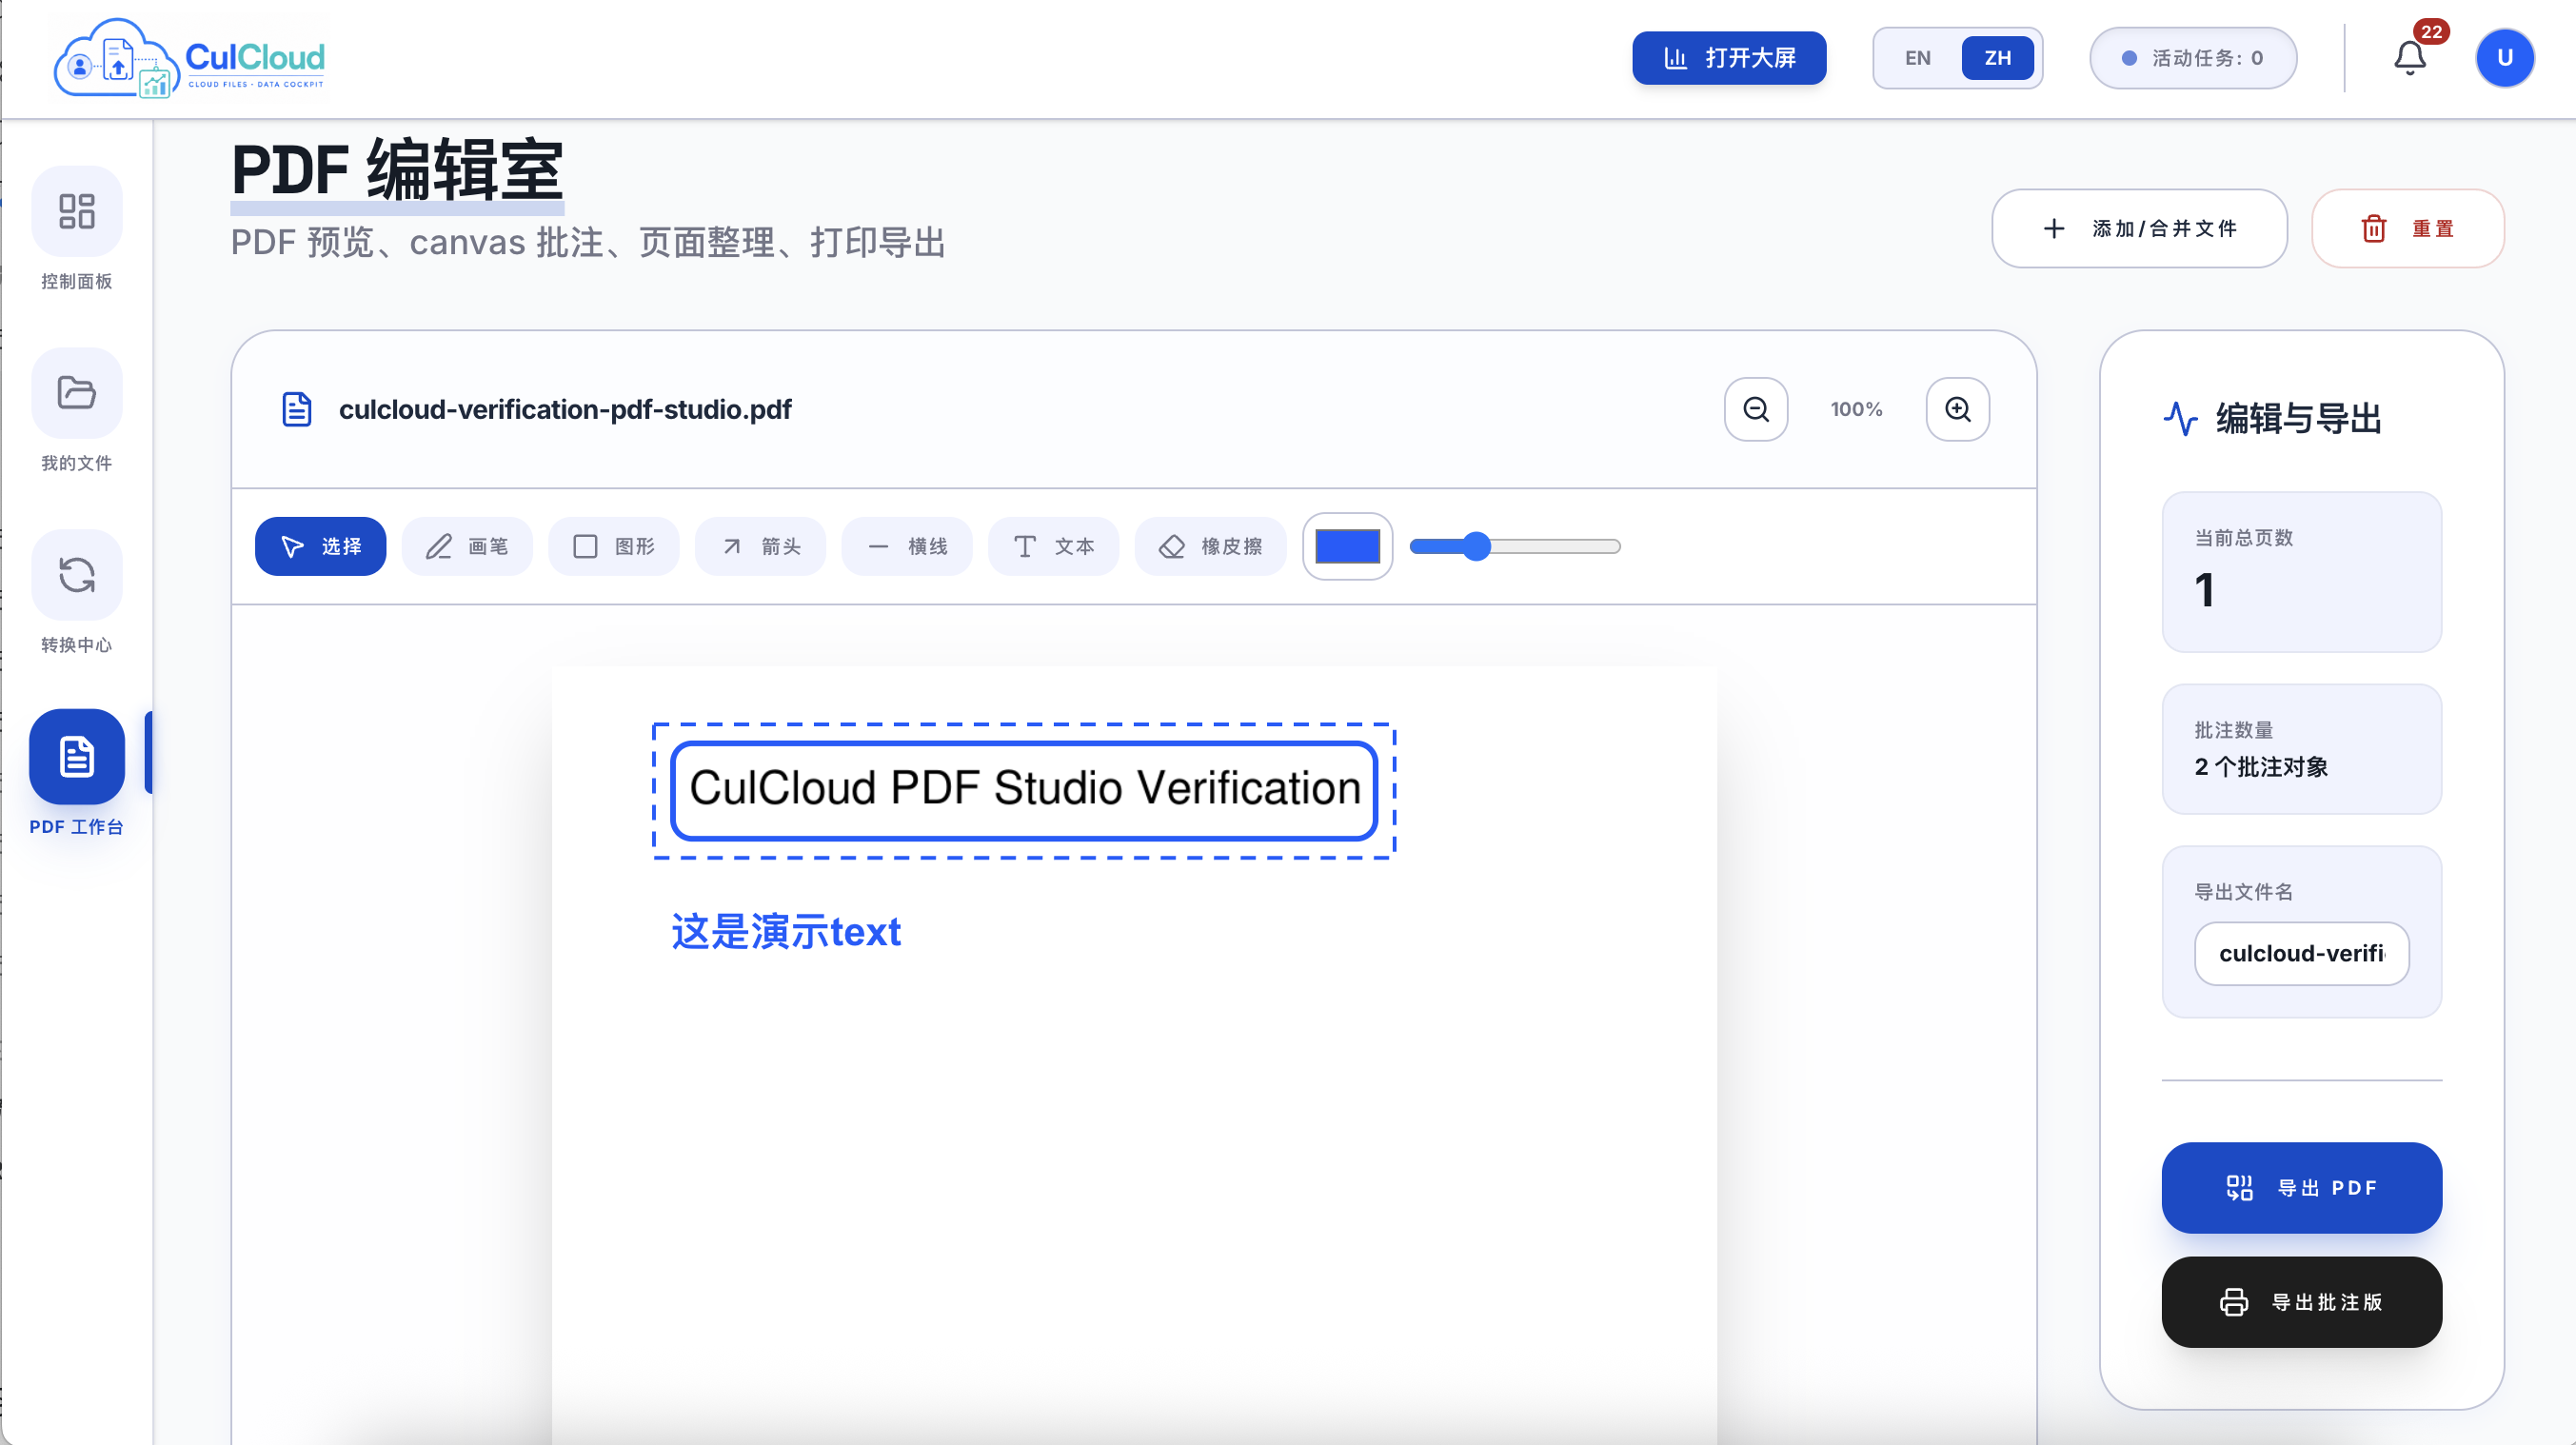
\includegraphics[width=\linewidth,height=0.25\textheight,keepaspectratio]{figures-png/ui/manual/fig05-manual-06-pdf-studio-annotation-workspace.png}
    \caption{页面与批注工作区}
  \end{subfigure}
  \hfill
  \begin{subfigure}{0.48\textwidth}
    \centering
    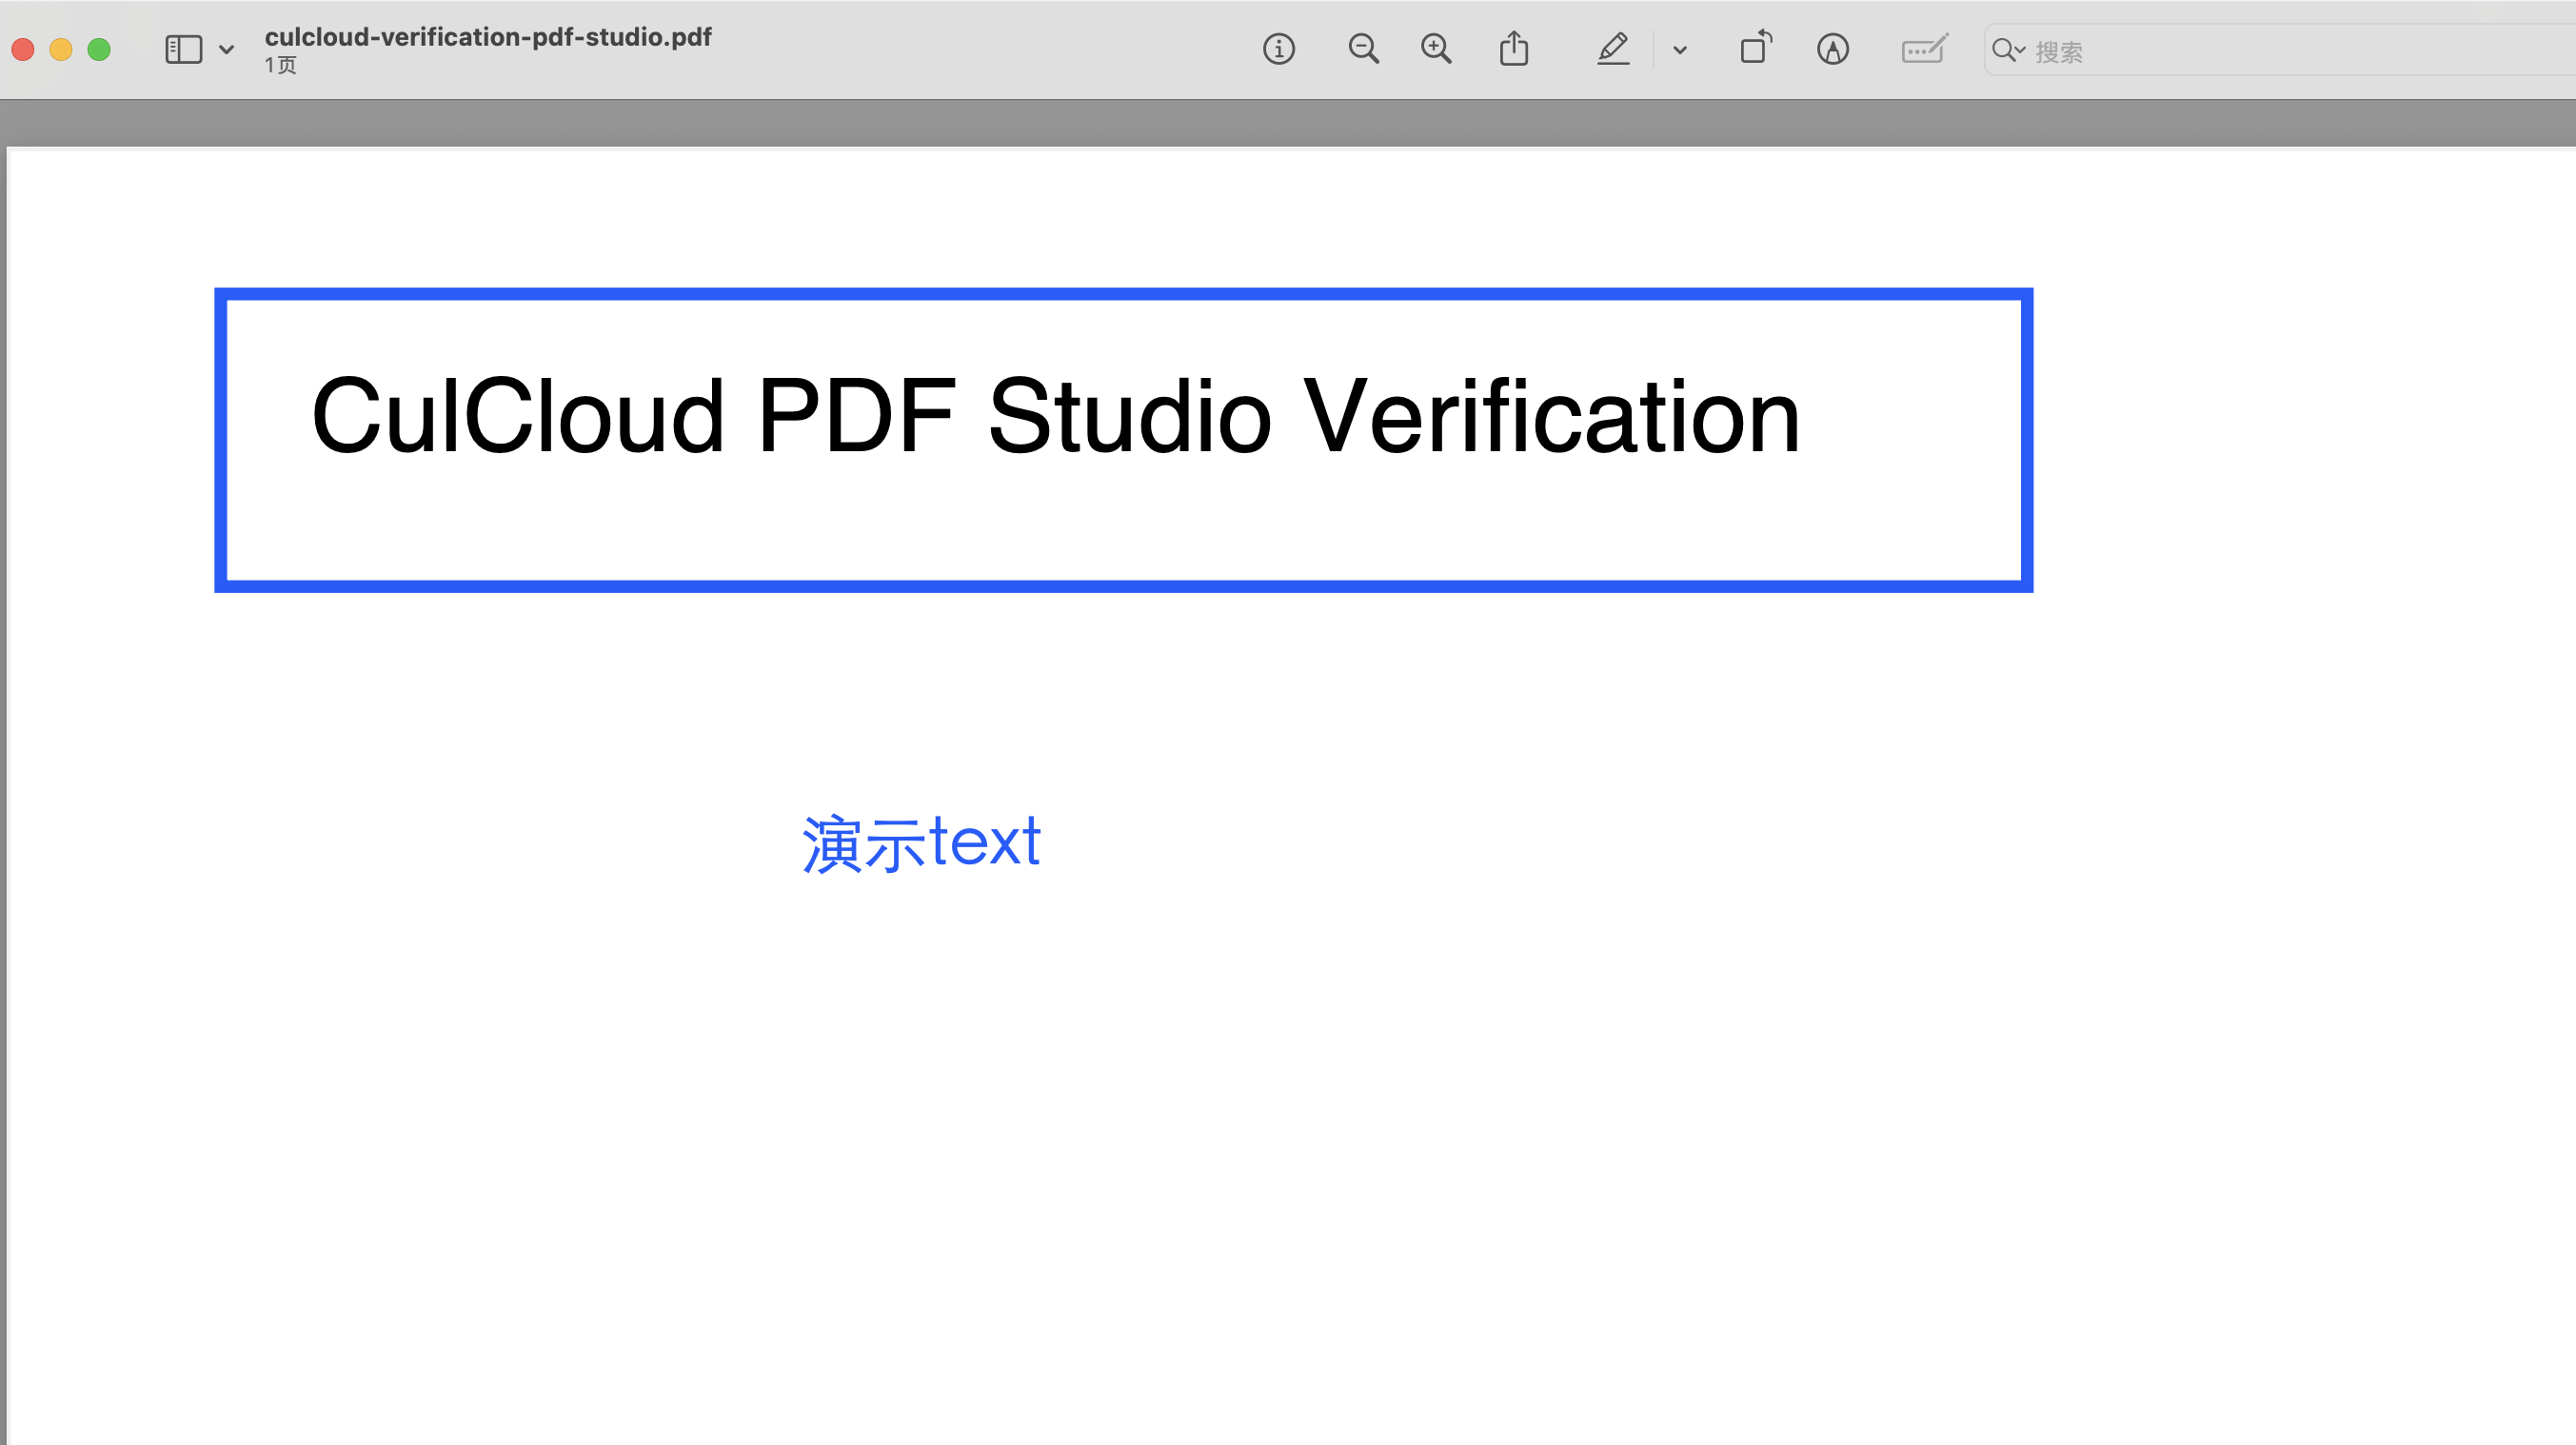
\includegraphics[width=\linewidth,height=0.25\textheight,keepaspectratio]{figures-png/ui/manual/fig05-manual-10-pdf-export-opened-result.png}
    \caption{导出后文件结果}
  \end{subfigure}
  \caption{PDF 编辑室处理结果图}
  \label{fig:chap05-pdf-manual-group}
\end{figure}

\section{管理驾驶舱模块的实现}

\subsection{实时运行视图}

管理驾驶舱由 \texttt{Analytics.tsx} 和 \texttt{AnalyticsSlides.tsx} 实现。第一屏通过 \texttt{useBizData} 直接读取 FastAPI 的实时接口，包括 \texttt{/api/v1/files}、\texttt{/api/v1/tasks/stats}、\texttt{/api/v1/tasks/queue-length}、\texttt{/api/v1/logs/timeline}、\texttt{/api/v1/logs/stats} 和 \texttt{/api/v1/system/health}。这些数值会随用户端上传、转换、PDF 导出和日志写入而变化，是系统当前运行状态。

第一屏的实现目标是反映“现在系统发生了什么”。文件数量来自当前 MinIO 对象，任务成功率来自 Redis 任务统计，近期事件来自日志时间线，服务状态来自健康检查快照。用户端完成一次文件转换后，任务统计和事件列表应随轮询刷新而变化，这也是管理端与用户端互通的关键证据。

\subsection{历史分析视图}

第二屏和第三屏读取 Flask Analytics 提供的历史分析接口。Flask 服务从 \texttt{data/spark-output/*.json} 读取 Spark 聚合结果，包含历史文件样本、历史转换任务、历史文件类型分布、历史转换桑基图、历史有效遥测、历史数据质量、历史存储水位和历史错误热力图。该部分用于体现大数据分析链路，不与第一屏实时指标混用。

历史分析视图的价值在于展示离线聚合能力。Spark 脚本对遥测样本执行文件格式分布、转换矩阵、访问趋势、质量报告和错误热力图统计，Flask 只负责把聚合结果转成 API。由于历史样本与实时业务数据不是同一口径，页面标题和正文均明确标注“历史”，避免将样本规模误解为当前运行规模。

\begin{figure}[H]
  \centering
  \begin{subfigure}{0.32\textwidth}
    \centering
    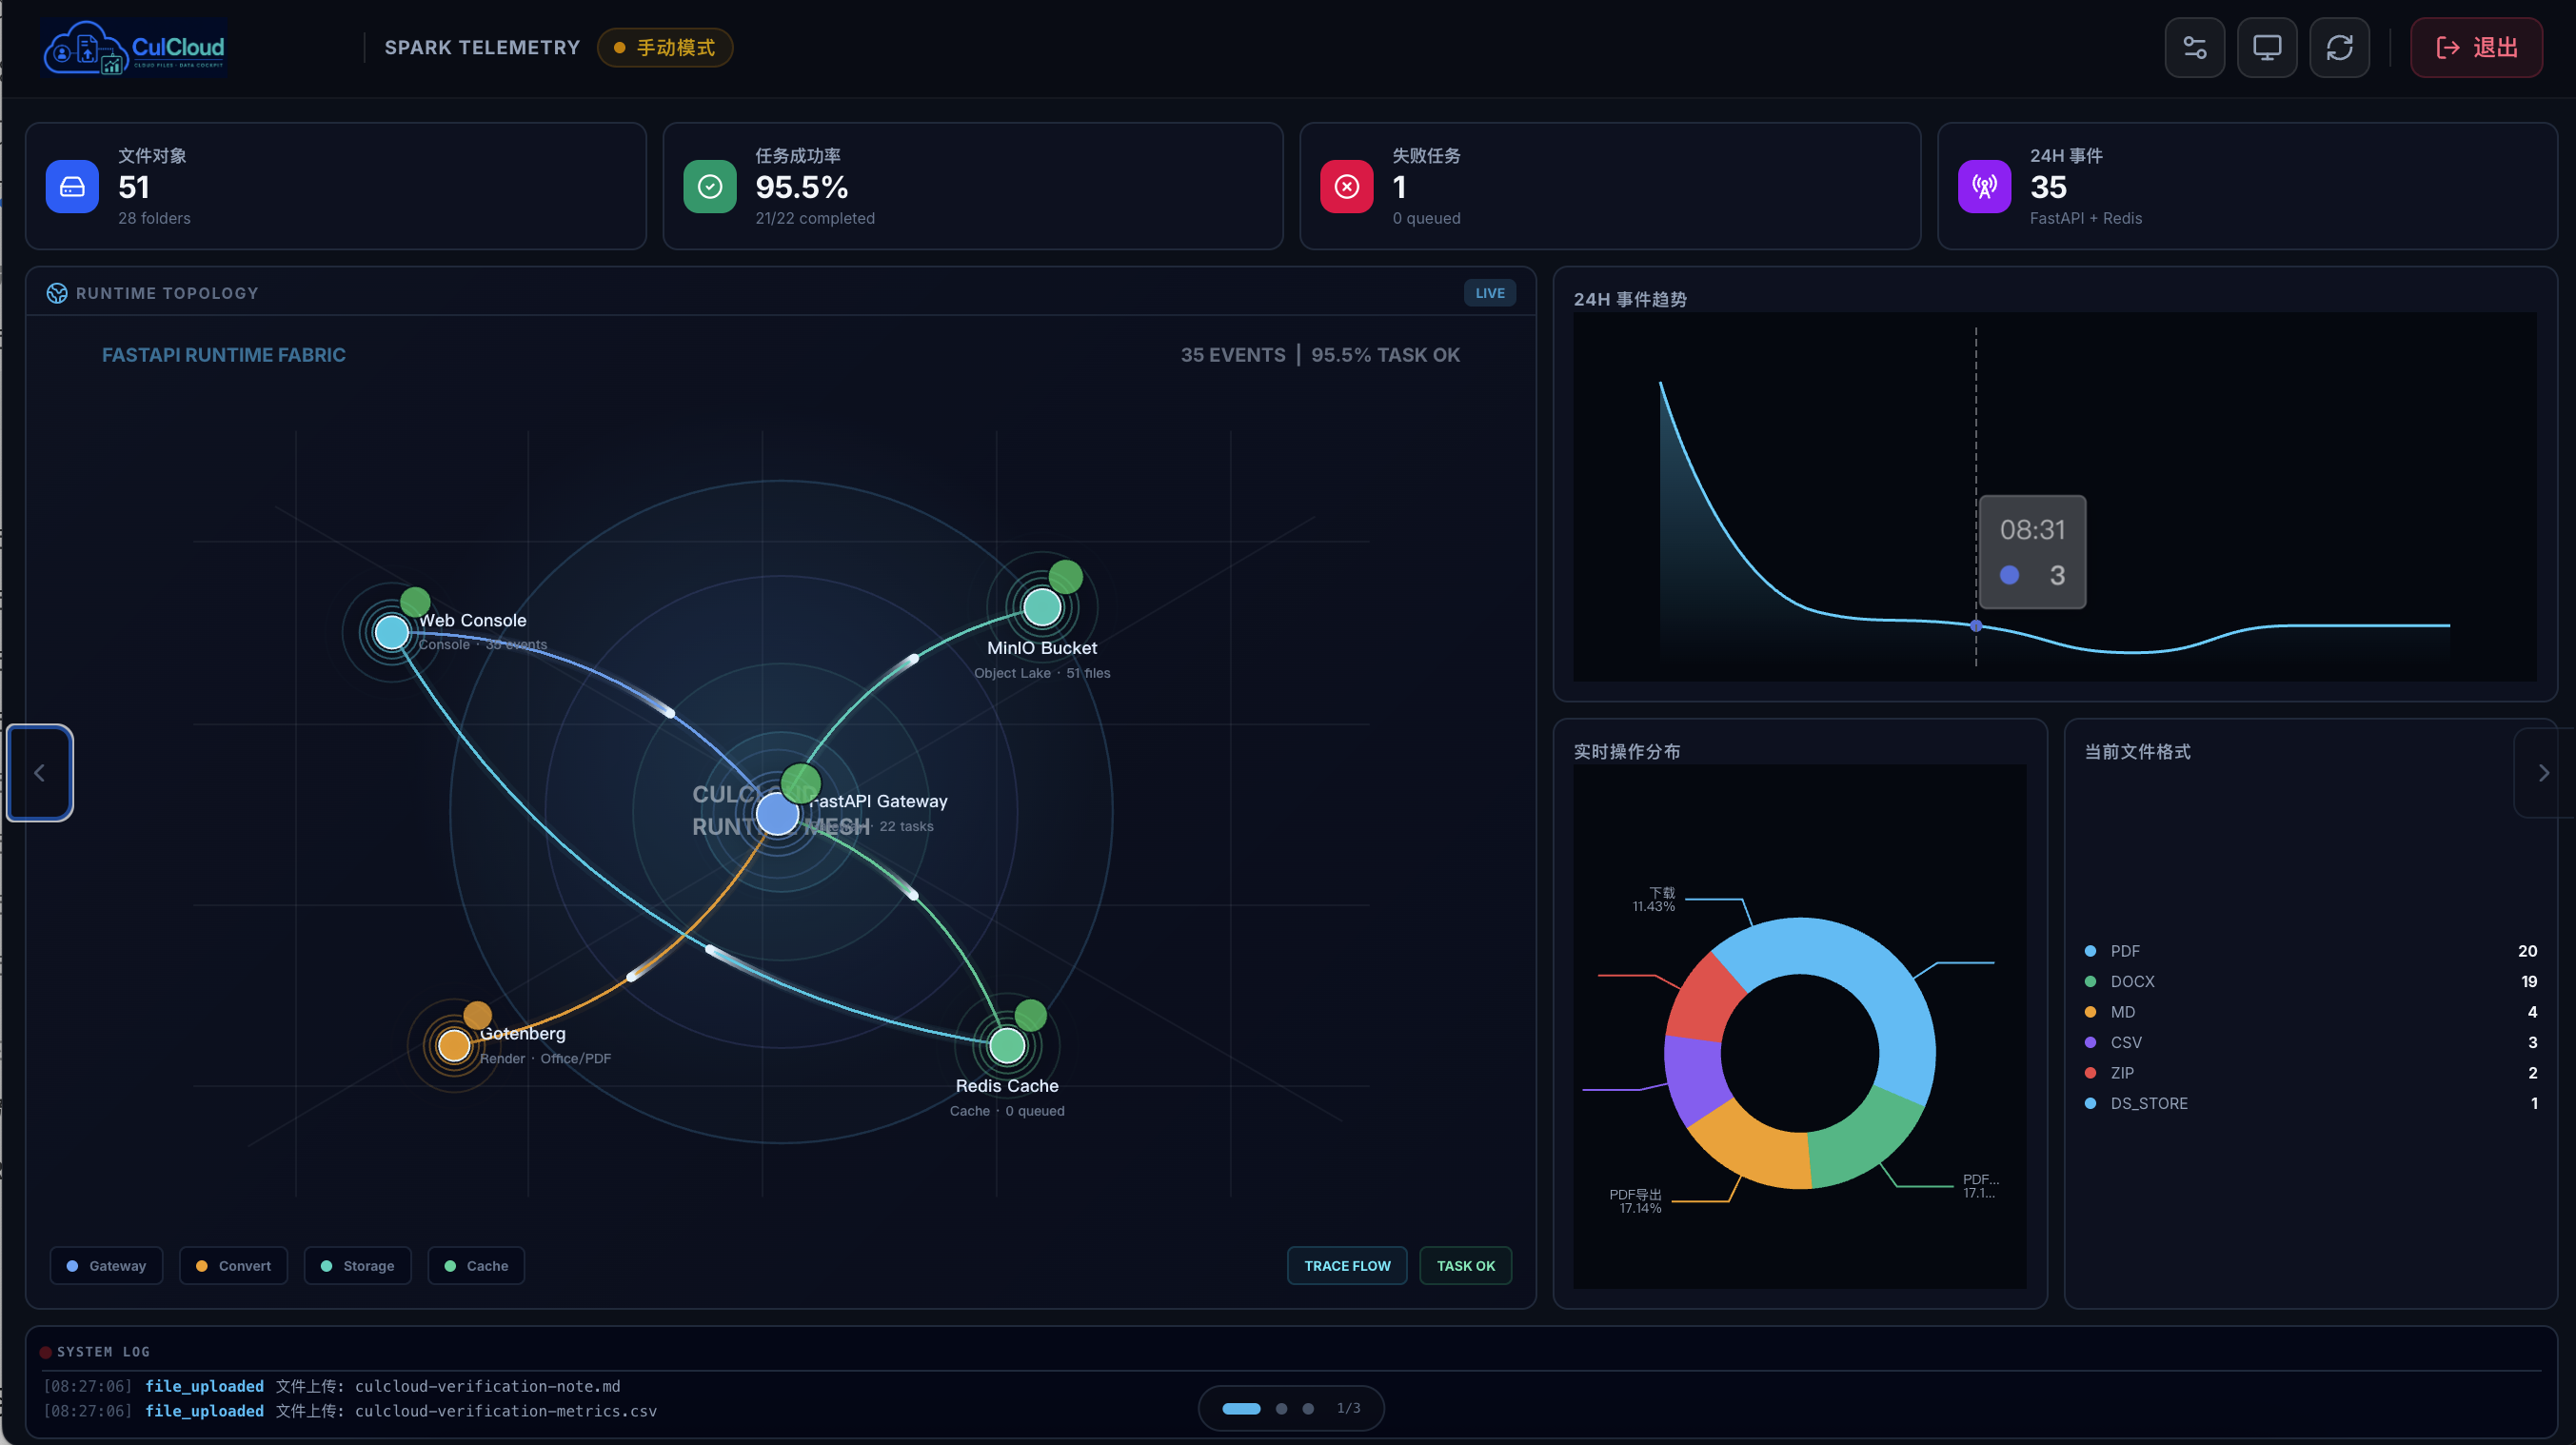
\includegraphics[width=\linewidth,height=0.20\textheight,keepaspectratio]{figures-png/ui/manual/fig05-manual-09-admin-runtime-topology-events.png}
    \caption{实时拓扑与事件}
  \end{subfigure}
  \hfill
  \begin{subfigure}{0.32\textwidth}
    \centering
    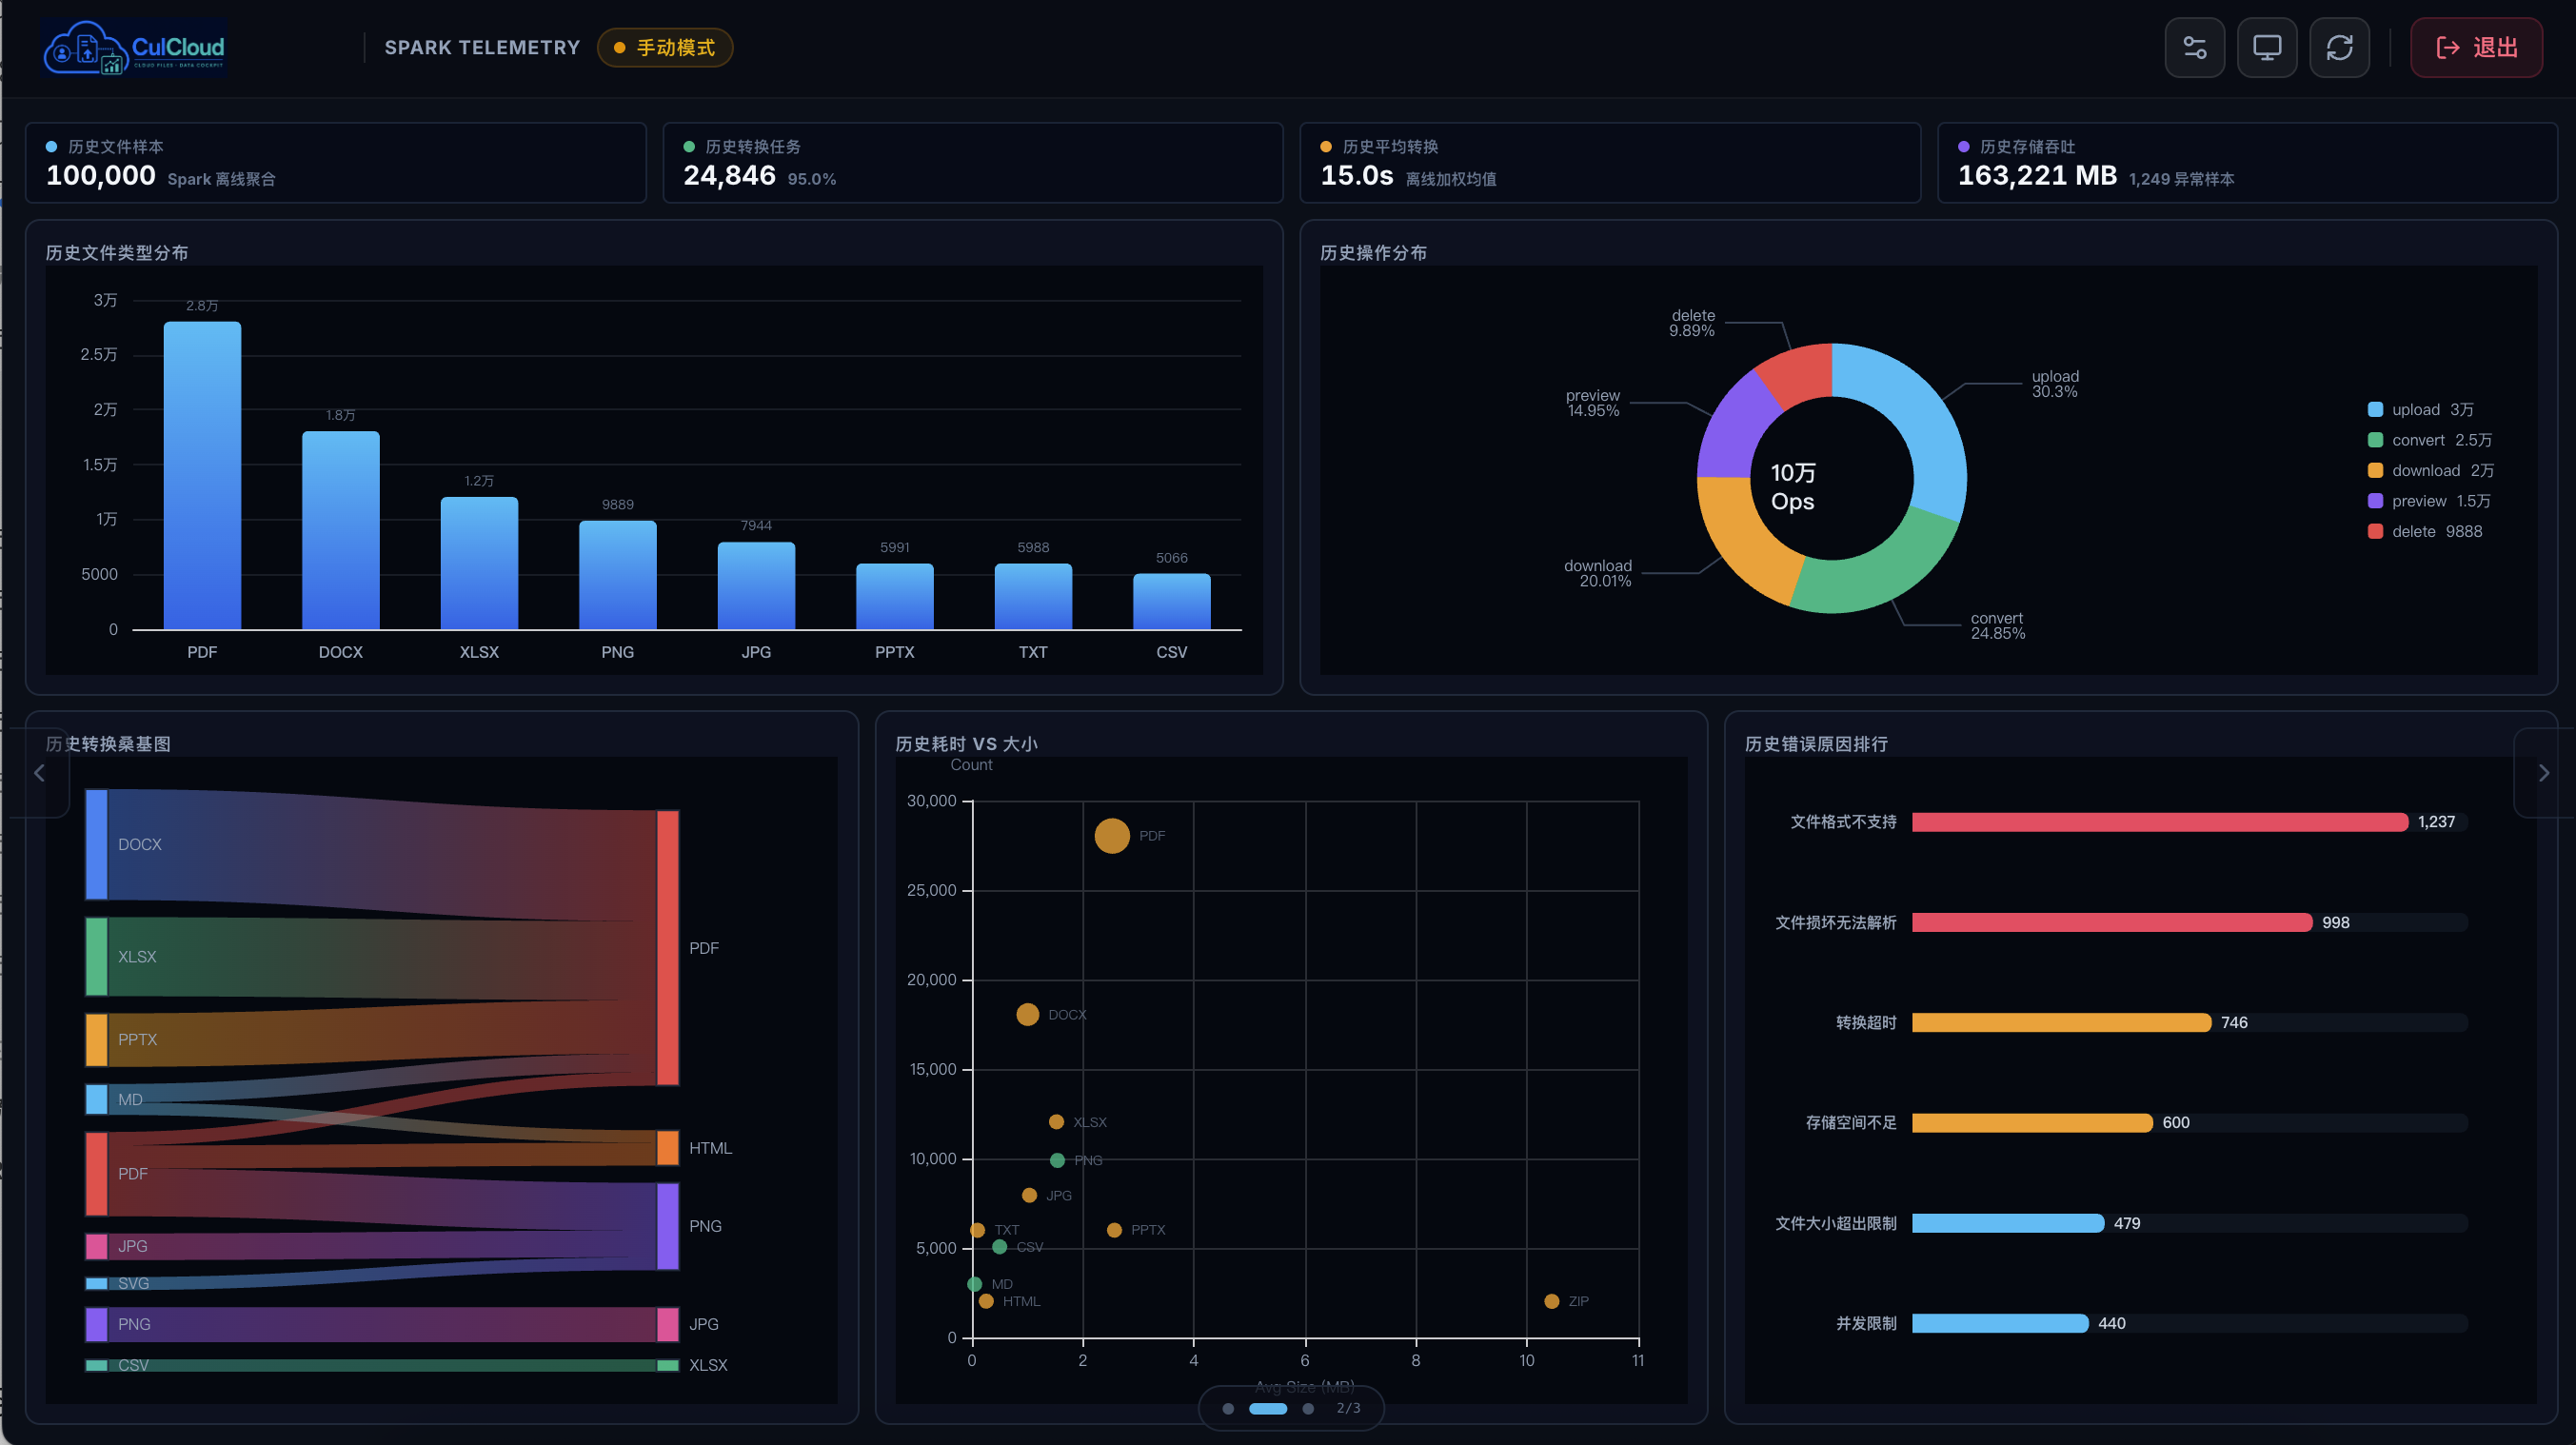
\includegraphics[width=\linewidth,height=0.20\textheight,keepaspectratio]{figures-png/ui/manual/fig05-manual-08-admin-historical-processing.png}
    \caption{历史转换分析}
  \end{subfigure}
  \hfill
  \begin{subfigure}{0.32\textwidth}
    \centering
    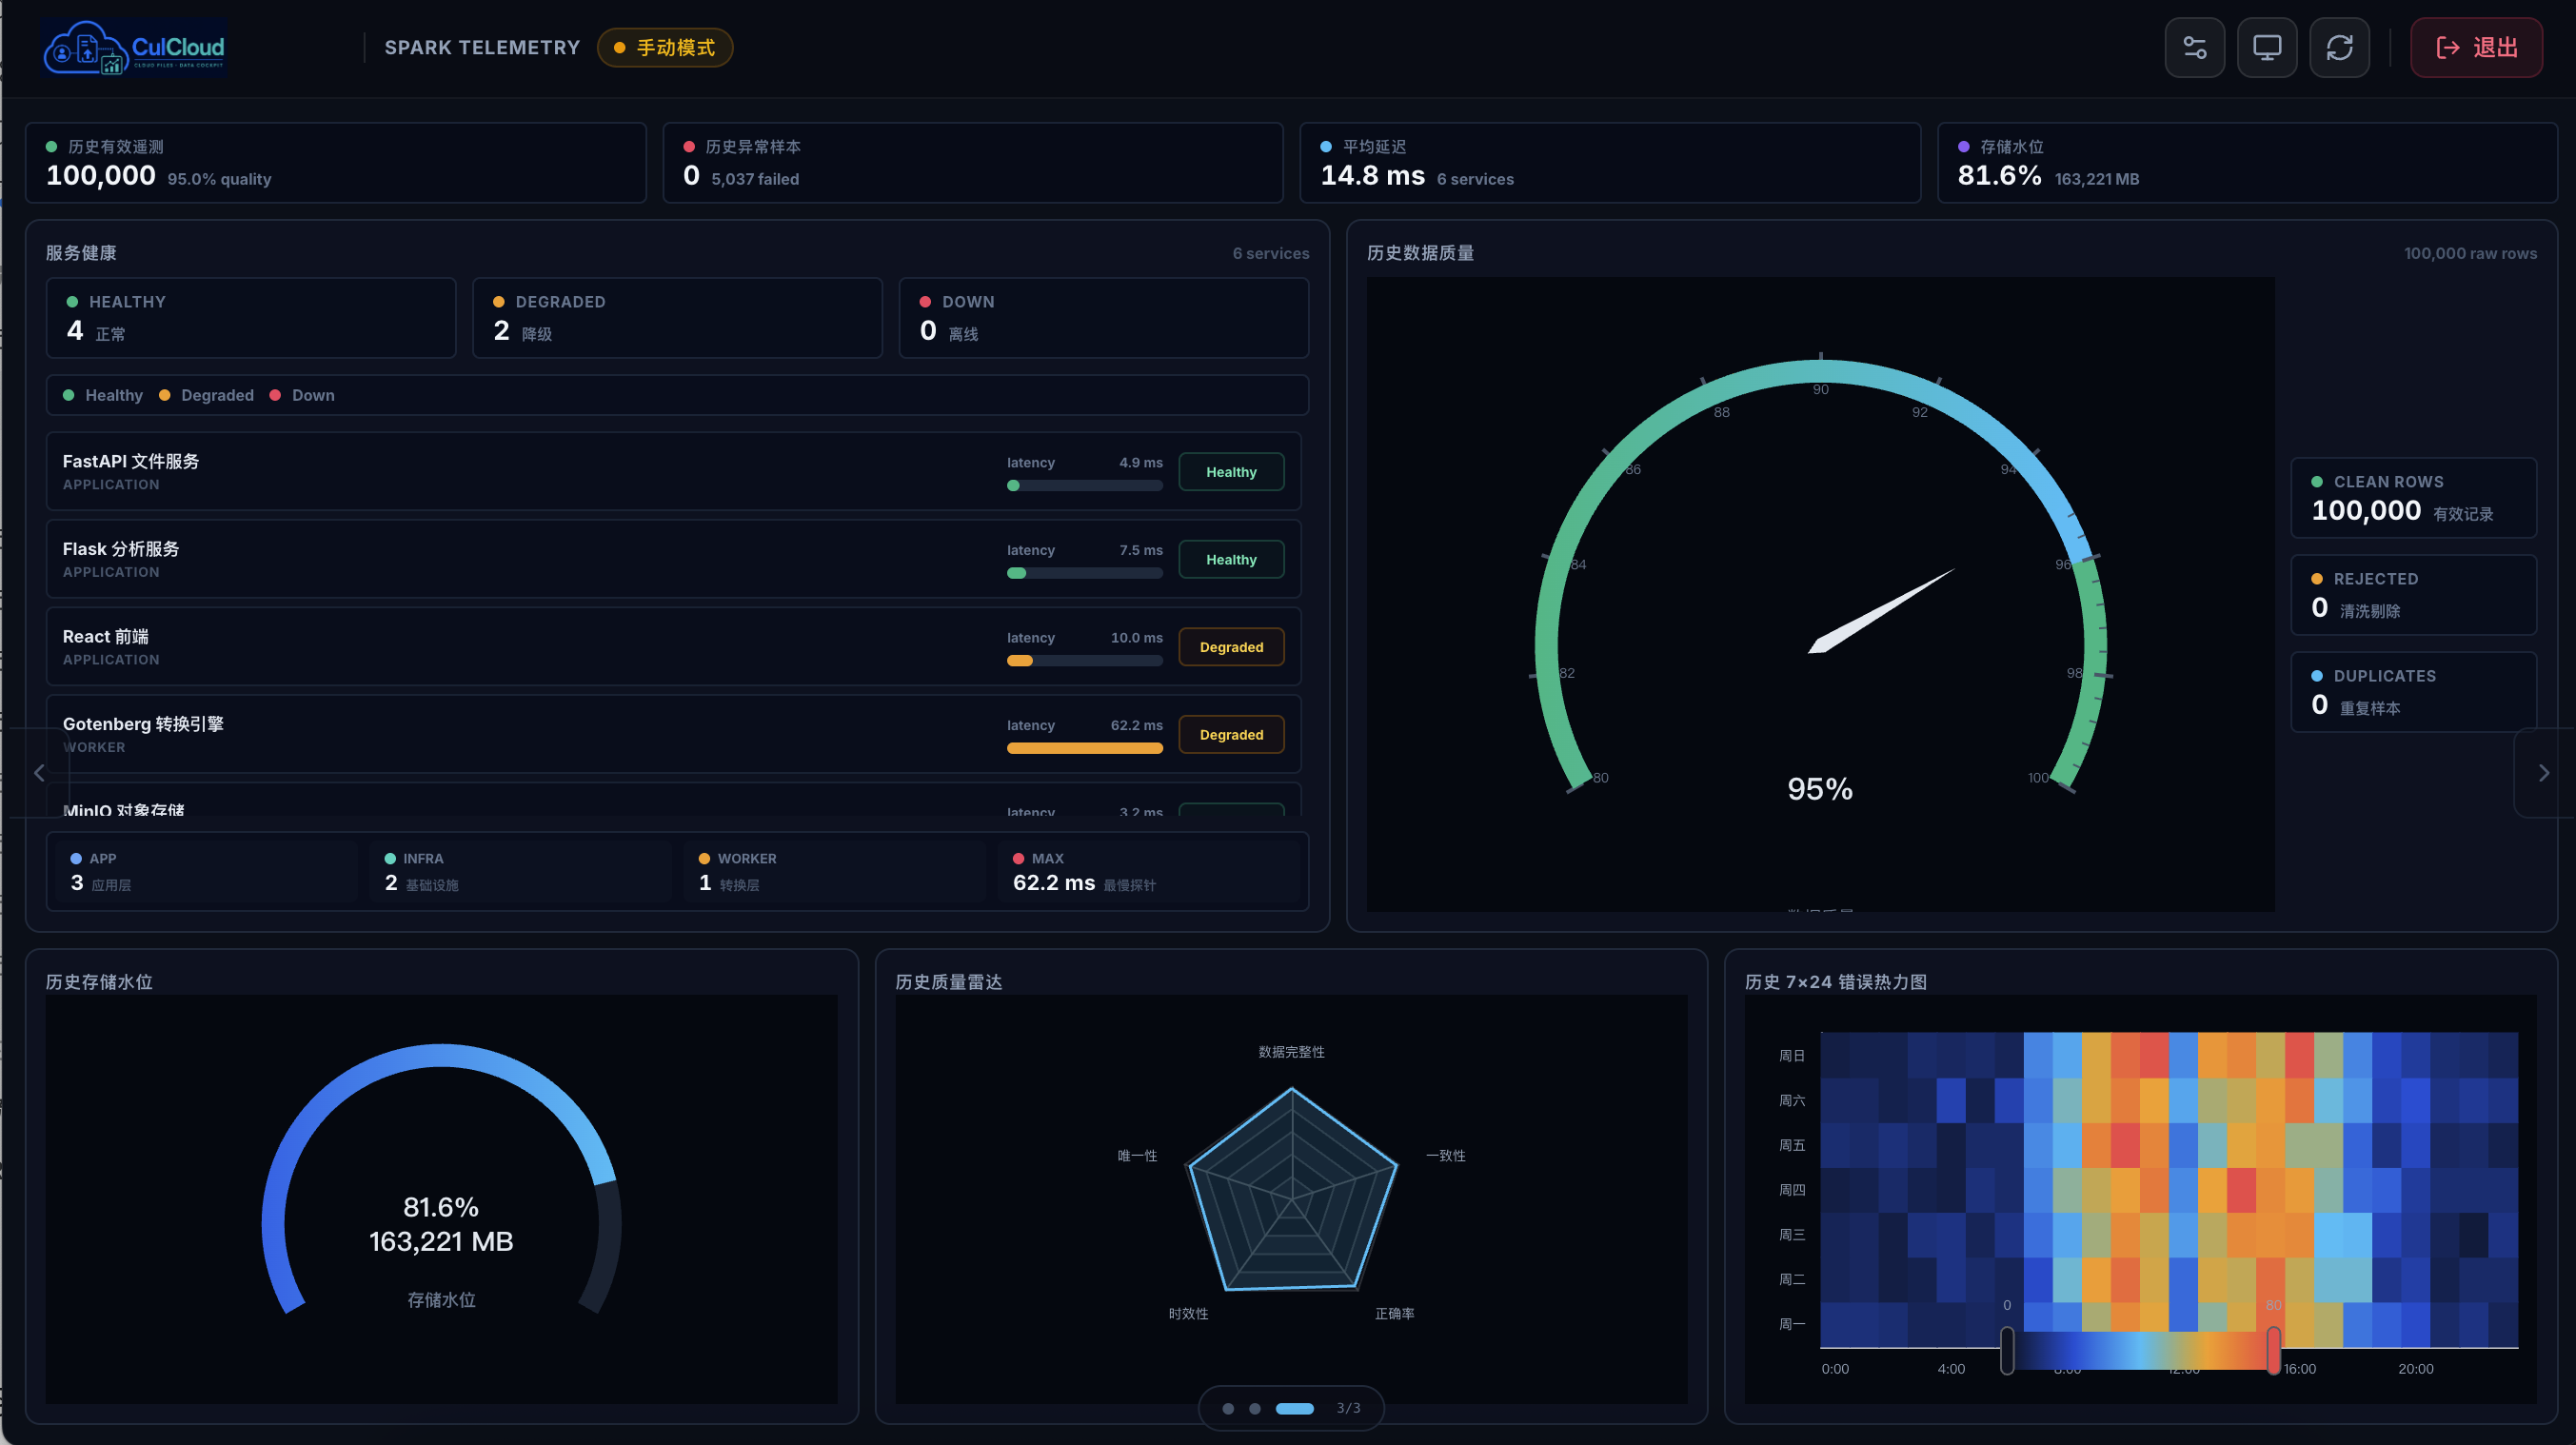
\includegraphics[width=\linewidth,height=0.20\textheight,keepaspectratio]{figures-png/ui/manual/fig05-manual-07-admin-historical-quality.png}
    \caption{历史质量分析}
  \end{subfigure}
  \caption{管理驾驶舱运行与历史分析结果图}
  \label{fig:chap05-admin-manual-group}
\end{figure}

\section{本章小结}

本章围绕真实代码位置说明了个人首页、我的文件、文件预览、转换中心、PDF 编辑室和管理驾驶舱的实现方式。系统实现的核心特点是前端视图、API 客户端、后端路由、领域服务、MinIO 对象和 Redis 状态之间形成清晰链路，使用户端操作能够产生可查询任务、可下载产物和管理端可观察数据。

\chapter{总结与展望}

\section{工作总结}

本项目围绕"大数据分析与可视化"这一主题，设计并实现了一个基于 Spark 与 Flask 的大数据分析与可视化系统。通过本项目的实践，主要完成了以下工作：

\begin{enumerate}
  \item 成功搭建了基于 Docker 的 Hadoop + Spark 大数据开发环境；
  \item 实现了基于 Spark SQL 的数据 ETL 处理和多维度分析流水线；
  \item 构建了基于 Flask 的 RESTful API 服务，提供标准化的数据访问接口；
  \item 开发了基于 React + ECharts 的可视化仪表盘，实现了分析结果的直观展示；
  \item 形成了完整的课程大作业技术文档，为后续学习和工作积累了经验。
\end{enumerate}

\section{不足与展望}

尽管本系统实现了基本的大数据分析与可视化功能，但仍存在以下不足：

\begin{itemize}
  \item \textbf{实时性不足}：当前系统主要面向离线批处理场景，未来可引入 Spark Streaming 实现实时数据处理；
  \item \textbf{分析维度有限}：当前仅实现了基础的数据分析功能，未来可引入更多高级分析算法，如聚类分析、关联规则挖掘等；
  \item \textbf{交互性有待提升}：前端可视化交互功能相对简单，未来可增加数据下钻、联动筛选等交互功能；
  \item \textbf{自动化程度不足}：数据采集、处理任务调度等流程尚未完全自动化，未来可引入 Airflow 等调度框架实现工作流自动化。
\end{itemize}

\section{心得体会}

通过本次课程大作业的实践，加深了对大数据技术栈的理解，特别是对 Hadoop 分布式存储、Spark 分布式计算、Flask Web 服务、前端可视化等技术的综合运用有了更为深入的认识。同时，在项目开发过程中也锻炼了问题分析和解决能力，为今后从事大数据相关领域的工作打下了基础。

\chapter{总结与展望}

本章对 CulCloud 云盘与大数据分析平台的设计与实现工作进行总结，并说明系统当前不足和后续改进方向。

\section{总结}

\subsection{系统功能成果}

本文围绕 CulCloud 云盘与大数据分析平台完成了系统设计、前端实现、文件处理、PDF 编辑室、任务监控和文档工程规划。项目实现了真实首页指标、拖拽上传、文件夹管理、文件分类、专门文件预览页、PDF canvas 批注、页面整理、打印导出和管理端遥测分析。

\subsection{课程实践成果}

项目将大数据分析、云存储、任务队列、文件转换和前端可视化结合起来，能够支撑课程大作业演示和报告撰写。系统中的上传、转换、预览和失败记录也为后续 Spark 聚合分析提供了数据来源。

\section{不足之处}

\subsection{PDF 批注写回不足}

当前 PDF 工作台的批注功能主要在前端 Web 端的 Canvas 视图层及打印导出中生效，尚未实现将用户的绘图 and 文本批注直接持久化写回 PDF 底层文件结构中。其核心技术成因在于：一是 PDF 规范采用笛卡尔坐标系（原点在左下角），而前端 Canvas 容器采用逻辑像素坐标系（原点在左上角），在页面缩放与旋转时需要进行复杂的仿射变换矩阵计算；二是系统缺乏中文字体的子集化嵌入机制，强行写回会导致不同终端查看时因缺少中文字体而无法正确显示字符；三是涉及 PDF 增量更新与注解对象（Annotation Object）字典树的序列化写回算法尚未在后端服务中实现，难以保证 PDF 文件的二进制结构合规与历史版本兼容。

\subsection{Office 深度预览不足}

由于现代浏览器无法原生解析并高保真呈现微软 Office 办公套件格式，系统在处理此类文件时，必须采用静默调用 Gotenberg 后端服务将其转换为 PDF 并写入 Redis 缓存库的过渡方案。这一方案深度依赖转换引擎的单点可用性。在 Gotenberg 容器发生宕机、转换任务队列发生阻塞或面对超大尺寸文件时，系统缺乏成熟的降级重试与故障平滑恢复机制，极易导致前端预览界面无限期处于加载状态，进而削弱了预览链路在极端高负载下的可用性。

\subsection{权限与协作能力不足}

云盘分享、多人协作、权限体系和生产级鉴权未纳入本次课程项目范围。当前系统更适合单用户课程演示场景，距离多人协同云盘仍有差距。

\section{展望}

\subsection{增强 PDF 编辑能力}

后续计划引入 Fabric.js 构建更具交互性的富文本批注图层，替代目前基于简单 HTML5 Canvas 的手写体涂鸦。在此基础上，借助 pdf-lib 库在 Node.js 服务端重构批注的合规写回引擎，确保用户的几何标注、高亮文本与中文批注能够以标准注释对象的形式注入 PDF 二进制结构中。同时，优化多终端的批注缩放自适应算法，提供批注节点的增删改查和版本历史回溯服务。

\subsection{完善多格式文件处理}

后续可继续完善 Office、音频、视频、压缩包和大文件的上传、预览与转换策略，并通过更完整的白盒测试保证转换链路稳定。

\subsection{扩展数据分析指标}

未来将在数据分析大屏中引入更深度的 Spark 离线计算与实时遥测指标，深入评估接口每秒查询率（QPS）和数据质量瓶颈。通过精细化采集文件传输耗时、转换队列排队时长以及不同格式文件解析的出错率，运用 Spark 分析多维度的性能瓶颈点，为底层 Gotenberg 转换实例的水平扩容以及 Redis 缓存淘汰策略 of 动态调整提供量化决策支撑。

\begin{acknowledgements}
  在本项目完成之际，首先要感谢江亮老师在课程学习与项目实践中的悉心指导和宝贵建议。江老师深入浅出的讲解使我们对大数据技术有了系统的认识，为项目的顺利开展奠定了坚实的理论基础。

  感谢课程小组各位成员的共同努力和密切协作，大家在项目开发过程中相互帮助、共同进步，顺利完成了系统的设计与实现。

  感谢常州工学院为我们提供了良好的学习环境和实验条件，使我们能够将理论知识转化为实践成果。

  最后，感谢所有在学习和生活中给予关心和支持的家人和朋友。
\end{acknowledgements}

% 参考文献
\bibliography{ref/refs}  % 参考文献使用 BibTeX 编译
% \printbibliography       % 参考文献使用 BibLaTeX 编译

% 附录
%\appendix
%\input{data/appendix}


\end{document}
